\RequirePackage{lineno}
\documentclass[aps,prd,twocolumn,showpacs,superscriptaddress,nofootinbib,floatfix,letterpaper]{revtex4-1}
\pdfoutput=1
\usepackage{placeins}
\usepackage{multirow}
\usepackage[utf8]{inputenc}
\usepackage{color}
% stuff before document begins.  

\RequirePackage[detect-all=true,group-digits=true,group-separator={,},binary-units=true]{siunitx}
\RequirePackage{xspace}
\RequirePackage{graphicx}
%\usepackage[pdftex,bookmarks,hidelinks, draft]{hyperref}
\usepackage[pdftex,bookmarks,hidelinks]{hyperref}

\graphicspath{ {graphics/} }
% This holds definitions of macros to enforce consistency in names.

% This file is the sole location for such definitions.  Check here to
% learn what there is and add new ones only here.  

% also see units.tex for units.  Units can be used here.

%%% Common terms

% Check here first, don't reinvent existing ones, add any novel ones.
% Use \xspace.

\newcommand{\bigo}[1]{\ensuremath{\mathcal{O}(#1)}}


% Things about oscillation
%
\newcommand{\numu}{\ensuremath{\nu_\mu}\xspace}
\newcommand{\nue}{\ensuremath{\nu_e}\xspace}
\newcommand{\nutau}{\ensuremath{\nu_\tau}\xspace}

\newcommand{\anumu}{\ensuremath{\bar\nu_\mu}\xspace}
\newcommand{\anue}{\ensuremath{\bar\nu_e}\xspace}
\newcommand{\anutau}{\ensuremath{\bar\nu_\tau}\xspace}

\newcommand{\dm}[1]{\ensuremath{\Delta m^2_{#1}}\xspace} % example: \dm{12}

\newcommand{\sinst}[1]{\ensuremath{\sin^2\theta_{#1}}\xspace} % example \sinst{12}
\newcommand{\sinstt}[1]{\ensuremath{\sin^22\theta_{#1}}\xspace}  % example \sinstt{12}

\newcommand{\deltacp}{\ensuremath{\delta_{\rm CP}}\xspace}   % example \deltacp
\newcommand{\mdeltacp}{\ensuremath{\delta_{\rm CP}}}   %%%%%%%%%%  <--- missing something; what's the m for?

\newcommand{\nuxtonux}[2]{\ensuremath{\nu_{#1} \to \nu_{#2}}\xspace}  % example \nuxtonux23 (no {...} )
\newcommand{\numutonumu}{\nuxtonux{\mu}{\mu}}
\newcommand{\numutonue}{\nuxtonux{\mu}{e}}
% Add chi sqd MH?  avg delta chi sqd?

\newcommand{\numubartonumubar}{
\ensuremath{\overline{\numu}\rightarrow\overline{\numu}}\xspace
}

\newcommand{\numubartonuebar}{
\ensuremath{\overline{\numu}\rightarrow\overline{\nue}}\xspace
}
% atmospheric neutrinos and PDK
\newcommand{\ptoknubar}{\ensuremath{p\rightarrow K^+ \overline{\nu}}\xspace}
\newcommand{\ptoepizero}{\ensuremath{p \rightarrow e^+ \pi^0}\xspace}
\newcommand{\ntoek}{\ensuremath{n\rightarrow e^{-}K^{+}}\xspace}
\newcommand{\nnbar}{\ensuremath{n-\bar{n}}\xspace}



% Isotopes - stay here
\def\argon40{${}^{40}$Ar}       
\def\Ar39{$^{39}$Ar}
\def\Cl40{$^{40}$Cl}
\def\K40{$^{40}$K}
\def\B8{$^{8}$B}
\newcommand\isotope[2]{\textsuperscript{#2}#1} % use as, e.g.,: \isotope{Si}{28}

% Parameters common to SP DP
\def\ndfromtarget{\SI{574}{\meter}\xspace} % ND from target
\def\fdfiducialmass{\SI{40}{\kt}\xspace}
\def\driftvelocity{\SI{1.6}{\milli\meter/\micro\second}\xspace} % same for sp and dp?
\def\lartemp{\SI{88}\,K\xspace}
\def\larmass{\SI{17.5}{\kt}\xspace} % full mass in cryostat
\def\cryostatht{\SI{17.8}{\meter}\xspace} % outer height of cryostat (Jim Stewart 5/2/19)
\def\cryostatlen{\SI{65.8}{\meter}\xspace} % length of cryostat (Jim Stewart 5/2/19)
\def\cryostatwdth{\SI{18.9}{\meter}\xspace} % width of cryostat (Jim Stewart 5/2/19)
\def\nominalmodsize{\SI{10}{kt}\xspace} % nominal module size 10 kt
\def\dunelifetime{\SI{20}{years}\xspace} % nominal operational life time of DUNE experiment
\def\pipiibeampower{\SI{1.2}{MW}\xspace} 
\def\cooldown{cool-down\xspace} % standardize w/ or w/o space or hyphen

% Parameters SP
\def\spmaxfield{\SI{500}{\volt/\centi\meter}\xspace} % SPfield strength
\def\spactivelarmass{\SI{10}{\kt}\xspace} % active mass in cryostat
\def\spmaxdrift{\SI{3.5}{\m}\xspace}
\def\tpcheight{\SI{12.0}{\meter}\xspace} % height of SP TPC, APA, CPA and of DP TPC
\def\sptpclen{\SI{58.2}{\meter}\xspace} % length of SP TPC, APA, CPA
\def\apacpapitch{\SI{2.3}{\meter}\xspace} % pitch of SP CPAs and APAs
\def\spfcmodlen{\SI{3.5}{\m}} % length of SP FC module
\def\spnumch{\num{384000}\xspace} % total number of APA readout channels 
\def\spnumpdch{\num{6000}\xspace} % total number of PD readout channels 
\def\planespace{\SI{4.8}{\milli\meter}\xspace}
\def\sptargetdriftvolt{$-\SI{180}{\kilo\volt}$\xspace} % target drift voltage - positive
\def\sptargetdriftvoltpos{\SI{180}{\kilo\volt}\xspace} % target drift voltage - positive
\def\coldbox{cold box\xspace} % standardize w/ or w/o space or hyphen
\def\Coldbox{Cold box\xspace} % standardize w/ or w/o space or hyphen
\def\endwall{end wall\xspace} % standardize w/ or w/o space

% Parameters DP
\def\dpactivelarmass{\SI{12.1}{\kt}\xspace} % active mass in cryostat
\def\dpfidlarmass{\SI{10.6}{\kt}\xspace} % fiducial mass in cryostat
\def\dpmaxdrift{\SI{12}{\m}\xspace} % max drift length
\def\dptpclen{\SI{60}{\meter}\xspace} % length of TPC
\def\dptpcwdth{\SI{12}{\meter}\xspace} % width of TPC
\def\dpswchpercrp{\num{36}\xspace} % number of anode/lem sandwiches per CRP 
\def\dpnumswch{\num{2880}\xspace} % total number of anode sandwiches in module
\def\dptotcrp{\num{80}\xspace} % total number of CRPs in module
\def\dpchpercrp{\num{1920}\xspace} %  channels per CRP
\def\dpnumcrpch{\num{153600}\xspace} % total number of CRP channels in module
\def\dpchperchimney{\num{640}\xspace} %  channels per chimney  --CRP channels?
\def\dpnumpmtch{\num{720}\xspace} % number of PMT channels
\def\dpstrippitch{\SI{3.1}{\milli\meter}\xspace} % pitch of anode strips
\def\dpnumfcmod{\num{244}\xspace} % number of FC modules
\def\dpnumfcres{\num{240}\xspace} % number of FC resistors
\def\dpnumfcrings{\num{60}\xspace} % number of FC rings
\def\dpnominaldriftfield{\SI{500}{\volt/\cm}\xspace} % nominal drift voltage per cm
\def\dptargetdriftvoltpos{\SI{600}{\kV}\xspace} % target drift voltage - positive
\def\dptargetdriftvoltneg{\SI{-600}{\kV}\xspace} % target drift voltage - negative

% Nominal readout window time
%% SP has 2.25ms drift time.  The readout is 2*dt + 20%*dt extra.
\def\spreadout{\SI{5.4}{\ms}\xspace}
%% DP has 7.5 ms drift time.  The same (over generous) rule gives 16.5ms
\def\dpreadout{\SI{16.5}{\ms}\xspace}
% Supernova Neutrino Burst buffer and readout window time
\def\snbtime{\SI{100}{\s}\xspace}
% interesting amount of time we might have SNB neutrinos but not yet
% enough to trigger.
\def\snbpretime{\SI{10}{\s}\xspace}
% SP SNB dump size. MUST KEEP THIS MANUALLY IN SYNC 1.5 TB/s * \snbtime
\def\spsnbsize{\SI{45}{\TB}\xspace}

% available power in the CUC and for DAQ
\def\cucpower{\SI[inter-unit-product =$\cdot$]{500}{\kilo\volt\ampere}\xspace}
\def\daqpower{\SI[inter-unit-product =$\cdot$]{500}{\kilo\volt\ampere}\xspace}
\def\surfdaqpower{\SI[inter-unit-product =$\cdot$]{50}{\kilo\volt\ampere}\xspace}

% available racks in the CUC and for DAQ.
\def\cucracks{\SI{60}{racks}\xspace}
\def\daqracks{\SI{56}{racks}\xspace}
\def\surfdaqracks{\SI{8}{racks}\xspace}

% keep these three numerically in sync
\def\offsitepbpy{\SI{30}{\PB/\year}\xspace}
\def\offsitegbyteps{\SI{1}{\GB/\s}\xspace}
\def\offsitegbps{\SI{8}{\Gbps}\xspace}
\def\surffnalbw{\SI{100}{\Gbps}\xspace}



% New from Anne March/April 2018
%physics terms
\newcommand{\efield}{E field\xspace}
\newcommand{\Lbl}{Long-baseline\xspace}
\newcommand{\rms}{RMS\xspace} % Might want this small caps?
\newcommand{\threed}{3D\xspace}
\newcommand{\twod}{2D\xspace}
\newcommand{\fdth}{feedthrough\xspace} % ok not in gloss
\newcommand{\phel}{photoelectron\xspace} % ok not in gloss
\newcommand{\frfour}{FR-4\xspace} % used in gloss and sp hv chap



% Top-level requirements and specifications
% 1 Minimum drift field
\def\mindriftfield{\SI{250}{\volt/\cm}\xspace}
\def\mindriftfieldgoal{\SI{500}{\volt/\cm}\xspace}
% 2 FE elec noise
\def\elecnoisefe{ \SI{1000}{e$^-$}\xspace}
% 3 light yield
\def\lightyield{\SI{0.5}{pe/\MeV}\xspace}
\def\lightyieldgoal{\SI{5}{pe/\MeV}\xspace}
% 4 time resolution
\def\timeres{\SI{1}{\micro/\second}\xspace}
\def\timeresgoal{\SI{100}{ns}\xspace}
% 5 LAr purity
\def\larpurity{\SI{100}{ppt}\xspace}
\def\larpuritygoal{\SI{30}{ppt}\xspace}
% 6 APA gaps
\def\apagapsame{\SI{15}{\milli\m}\xspace}
\def\apagapdiff{\SI{30}{\milli\m}\xspace}
% 7 drift field uniformity (from component positioning)
\def\fielduniformity{\SI{1}{\%}\xspace}
% 8a APA collection wire angle
\def\apacollwireangle{$\SI{0}{^\circ}$\xspace}
% 8b APA induction wire angle
\def\apainducwireangle{$\pm\SI{35.7}{^\circ}$\xspace}
% 9a APA wire pitch - U,V
\def\uvpitch{\SI{4.7}{\milli\meter}\xspace}
% 9b APA wire pitch - X, G
\def\xgpitch{\SI{4.8}{\milli\meter}\xspace}
% 10 APA wire position tolerance
\def\wirepitchtol{$\pm$\SI{0.5}{\milli\meter}\xspace}
% 11 drift field uniformity (from HVS)
\def\fielduniformityhv{\SI{1}{\%}\xspace}
% 12 HV PS ripple contrib to noise
\def\hvripplenoise{\SI{100}{e$^-$}\xspace}
% 13 FE peaking time
\def\fepeaktime{\SI{1}{\micro\second}\xspace}
% 14 signal saturation level (SP)
\def\spsignalsat{\num{500000} electrons\xspace}
% 15 LAr N contamination
\def\nitrogencontam{\SI{25}{ppm}\xspace}
% 16 detector dead time
\def\deadtime{\SI{0.5}{\%}\xspace}
% Engineering
% 17 Cathode resistivity
\def\cathodemegohm{\SI{1}{\mega\ohm/square}\xspace}
\def\cathodegigohm{\SI{1}{\giga\ohm/square}\xspace}
% 
%\def\{\xspace}
% 19 ADC sampling frequency
\def\samplingfreq{\SI{2}{\mega\hertz}\xspace}
% 20 ADC dynamic range
\def\adcdynrange{\num{12} bits}  %{3000}:\num{1}\xspace}
\def\adcdynrangegoal{\num{13} bits} %{4070}:\num{1}\xspace}
% 21 CE power consumption (SP)
\def\cepower{\SI{50}{mW/channel}\xspace}
% 22 data to tape
\def\dataratetotape{\SI{30}{PB/year}\xspace}
% 23 SNB trigger
\def\snbtriggereff{90\% efficiency\xspace}
%\def\snbtriggervisenergy{90\% efficiency \xspace}
% 24 local E fields
\def\localefield{\SI{30}{\kV/\cm}\xspace}
% 25 non-FE noise contributions
\def\elecnoisenonfe{$<<$ \SI{1000}{e$^-$}\xspace}
% 26 impurity contrib from components
\def\larpuritycomps{$<<$ \SI{30}{ppt}\xspace}
% 28 dead channels
\def\deadchannels{\SI{1}{\%}\xspace}



% The following from phys ch-bsm 1/3/19 (was in their cls file)
\newcommand{\lsim}{{\;\raise0.3ex\hbox{$<$\kern-0.75em\raise-1.1ex\hbox{$\sim$}}\;}}
\newcommand{\gsim}{{\;\raise0.3ex\hbox{$>$\kern-0.75em\raise-1.1ex\hbox{$\sim$}}\;}}
\newcommand{\beq}{\begin{equation}}
\newcommand{\eeq}{\end{equation}}
\newcommand{\bea}{\begin{eqnarray}}
\newcommand{\eea}{\end{eqnarray}}
\newcommand{\DF}{\Delta_{4}}
\mathchardef\minus="002D
\newcommand{\dk}[1]{\textcolor{red}{#1}}
\newcommand{\dkc}[1]{\textbf{\textcolor{red}{(#1 --DK)}}}
\newcommand{\dd}[1]{\textcolor{blue}{#1}}

%Milestones (from Eric's talk Mar 12, 2019} https://indico.fnal.gov/event/20149/contribution/0/material/slides/1.pdf
\newcommand{\startpduneiispinstall}{March 2021\xspace}% Start of ProtoDUNE-II (SP) Installation: March 2021
\newcommand{\startpduneiidpinstall}{March 2022\xspace}%Start of ProtoDUNE-II (DP) Installation: March 2022
\newcommand{\sdlwavailable}{April 2022\xspace}%South Dakota Logistics Warehouse Available: April 2022
\newcommand{\cucbenocc}{October 2022\xspace}% Beneficial Occupancy of Cavern 1/CUC: October 2022
\newcommand{\accesscuccountrm}{April  2023\xspace}% CUC Counting Room Accessible: April 2023
\newcommand{\accesstopfirstcryo}{January 2024\xspace}%Top of Far Detector #1 Cryostat Accessible: January 2024
\newcommand{\startfirsttpcinstall}{August 2024\xspace}%Start of Far Detector #1 TPC Installation: August 2024
\newcommand{\firsttpcinstallend}{May 2025\xspace}% End of Far Detector #1 TPC Installation: May 2025
\newcommand{\accesstopsecondcryo}{January 2025\xspace}%Top of Far Detector #2 Accessible: January 2025
\newcommand{\startsecondtpcinstall}{August 2025\xspace}%Start of Far Detector #2 TPC Installation: August 2025
\newcommand{\secondtpcinstallend}{May 2026\xspace}%End of Far Detector #2 TPC Installation: May 2026

\newcommand{\maincavernstartexc}{(get date)\xspace}% Start exc of detector cavern 1. needed for exec summ

%Mike Kordosky: the command below is used to refer to
% planned entries in the requirements table.
\newcommand{\rrt}[1]{\ifthenelse{\equal{#1}{}}{[RT:TBD]}{[RT:#1]}}
\newcommand{\beamturnon}{fix beam turn on date in defs.tex\xspace}

%%%%%%% Everything below here is DEPRECATED (4/30/19 AH) %%%%%%%%%%

% Names of expts or detectors -- all these go into glossary DEPRECATED
% in use
\newcommand{\cherenkov}{Cherenkov\xspace}  %nonaccel
\newcommand{\kamland}{KamLAND\xspace} %cisc dp
\newcommand{\superk}{Super--Kamiokande\xspace} %nonaccel, bsm
\newcommand{\hyperk}{Hyper--Kamiokande\xspace} %nonaccel
\newcommand{\microboone}{MicroBooNE\xspace} %used in cisc sp, hv, daq
\newcommand{\minerva}{MINERvA\xspace} %tools/meth, nuosc11
\newcommand{\nova}{NOvA\xspace} %lots
\newcommand{\lariat}{LArIAT\xspace} % calib,dppds
\newcommand{\argoneut}{ArgoNeuT\xspace} %nonaccel
%not in use
\newcommand{\kkande}{Kamiokande\xspace}  
\newcommand{\miniboone}{MiniBooNE\xspace}
\newcommand{\numi}{NuMI\xspace}
\newcommand{\larnd}{LAr ND\xspace}

% usage not checked for the rest 4/30/19
% Random -- all these go into glossary DEPRECATED
\newcommand{\lartpc}{LArTPC\xspace}
\newcommand{\globes}{GLoBES\xspace}
\newcommand{\larsoft}{LArSoft\xspace}
\newcommand{\snowglobes}{SNOwGLoBES\xspace}
\newcommand{\docdb}{DUNE DocDB\xspace}
\newcommand{\lbl}{long-baseline\xspace} %DEPRECATED

% also have in glossary; Glossary also has CERN, PSL, other big labs, etc. DEPRECATED
\newcommand{\fnal}{Fermilab\xspace} 
\newcommand{\surf}{SURF\xspace} 
\newcommand{\bnl}{BNL\xspace}
\newcommand{\anl}{ANL\xspace}
 
 %detectors and modules
% also have in glossary; THE FOLLOWING NINE TERMS ARE DEPRECATED 4/30/19
\newcommand{\detmodule}{detector module\xspace}
\newcommand{\dual}{DP\xspace}
\newcommand{\Dual}{DP\xspace}
\newcommand{\single}{SP\xspace}
\newcommand{\Single}{SP\xspace}
\newcommand{\dpmod}{DP detector module\xspace}
\newcommand{\spmod}{SP detector module\xspace}
\newcommand{\lar}{LAr\xspace}
\newcommand{\lntwo}{LN$_2$\xspace}  %used in sp-tpcelec 

%detector components SP and DP -- need to be in gloss; THESE 14 ITEMS DEPRECATED:
\newcommand{\dss}{DSS\xspace}
\newcommand{\hv}{high voltage\xspace}
\newcommand{\fcage}{field cage\xspace}
\newcommand{\fc}{FC\xspace}
\newcommand{\fcmod}{FC module\xspace}  %%%   don't need?
\newcommand{\topfc}{top FC\xspace}
\newcommand{\botfc}{bottom FC\xspace}
\newcommand{\ewfc}{endwall FC\xspace}
\newcommand{\pdsys}{PD system\xspace}
\newcommand{\phdet}{photon detector\xspace}
\newcommand{\sipm}{SiPM\xspace}
\newcommand{\pmt}{PMT\xspace}
\newcommand{\pwrsupp}{power supply\xspace}
\newcommand{\pwrsupps}{power supplies\xspace}
% This holds definitions of macros to enforce consistency in units.

% This file is the sole location for such definitions.  Check here to
% learn what there is and add new ones only here.  

% also see defs.tex for names.


% see
%  http://ctan.org/pkg/siunitx
%  http://mirrors.ctan.org/macros/latex/contrib/siunitx/siunitx.pdf

% Examples:
%  % angles
%  \ang{1.5} off-axis
%
%  % just a unit
%  \si{\kilo\tonne}
%
%  % with a value:
%  \SI{10}{\mega\electronvolt}

%  range of values:
% \SIrange{60}{120}{\GeV}

% some shorthand notation
%\DeclareSIUnit \MBq {\mega\Bq}
\DeclareSIUnit \s {\second}
\DeclareSIUnit \MB {\mega\byte}
\DeclareSIUnit \GB {\giga\byte}
\DeclareSIUnit \TB {\tera\byte}
\DeclareSIUnit \PB {\peta\byte}
\DeclareSIUnit \Mbps {\mega\bit/\s}
\DeclareSIUnit \Gbps {\giga\bit/\s}
\DeclareSIUnit \Tbps {\tera\bit/\s}
\DeclareSIUnit \Pbps {\peta\bit/\s}
\DeclareSIUnit \kton {\kilo\tonne} % changed  back to kton
\DeclareSIUnit \kt {\kilo\tonne}
\DeclareSIUnit \Mt {\mega\tonne}
\DeclareSIUnit \eV {\electronvolt}
\DeclareSIUnit \keV {\kilo\electronvolt}
\DeclareSIUnit \MeV {\mega\electronvolt}
\DeclareSIUnit \GeV {\giga\electronvolt}
\DeclareSIUnit \m {\meter}
\DeclareSIUnit \cm {\centi\meter}
\DeclareSIUnit \in {\inchcommand}
\DeclareSIUnit \km {\kilo\meter}
\DeclareSIUnit \kV {\kilo\volt}
\DeclareSIUnit \kW {\kilo\watt}
\DeclareSIUnit \MW {\mega\watt}
\DeclareSIUnit \MHz {\mega\hertz}
\DeclareSIUnit \mrad {\milli\radian}
\DeclareSIUnit \year {year}
\DeclareSIUnit \POT {POT}
\DeclareSIUnit \sig {$\sigma$}
\DeclareSIUnit\parsec{pc}
\DeclareSIUnit\lightyear{ly}
\DeclareSIUnit\foot{ft}
\DeclareSIUnit\ft{ft}
\DeclareSIUnit \ppb{ppb}
\DeclareSIUnit \ppt{ppt}
\DeclareSIUnit \samples{S}

\sisetup{inter-unit-product = \ensuremath{{}\cdot{}}}
%\def\ktyr{\si[inter-unit-product=\ensuremath{{}\cdot{}}]{\kt\year}\xspace}
\newcommand{\ktyr}{\si{\kt\year}\xspace}
%\def\Mtyr{\si[inter-unit-product=\ensuremath{{}\cdot{}}]{\Mt\year}\xspace}
\newcommand{\Mtyr}{\si{\Mt\year}\xspace}
%\def\msr{\si[inter-unit-product=\ensuremath{{}\cdot{}}]{\meter\steradian}\xspace}
\newcommand{\msr}{\si{\meter\steradian}\xspace}
%\def\ktMWyr{\si[inter-unit-product=\ensuremath{{}\cdot{}}]{\kt\MW\year}\xspace}
\newcommand{\ktMWyr}{\si{\kt\MW\year}\xspace}
% used for hyphen, obsolete now: \newcommand{\SIadj}[2]{\SI[number-unit-product = -]{#1}{#2}}
% change command definition Nov 2017 in case people copy e.g., \ktadj from CDR text.
% E.g., \ktadj{10} now renders the same as \SI{10}{\kt}
\newcommand{\SIadj}[2]{\SI{#1}{#2}}

% Adjective form of some common units (Nov 2107 changed to be same as normal form, no hyphen)
% "the 10-kt detector"

\newcommand{\ktadj}[1]{\SIadj{#1}{\kt}}
% "the 1,300-km baseline"
\newcommand{\kmadj}[1]{\SIadj{#1}{\km}}
% "a 567-keV endpoint"
\newcommand{\keVadj}[1]{\SIadj{#1}{\keV}}
% "Typical 20-MeV event"
\newcommand{\MeVadj}[1]{\SIadj{#1}{\MeV}}
% "Typical 2-GeV event"
\newcommand{\GeVadj}[1]{\SIadj{#1}{\GeV}}
% "the 1.2-MW beam"
\newcommand{\MWadj}[1]{\SIadj{#1}{\MW}}
% "the 700-kW beam"
\newcommand{\kWadj}[1]{\SIadj{#1}{\kW}}
% "the 100-tonne beam"
\newcommand{\tonneadj}[1]{\SIadj{#1}{\tonne}}
% "the 4,850-foot depth beam"
\newcommand{\ftadj}[1]{\SIadj{#1}{\ft}}
%

% Mass exposure, people like to put dots between the units
% \newcommand{\ktyr}[1]{\SI[inter-unit-product=\ensuremath{{}\cdot{}}]{#1}{\kt\year}}
% must make usage of \ktyr above consistent with this one before turning on

% Beam x mass exposure, people like to put dots between the units
\newcommand{\ktmwyr}[1]{\SI[inter-unit-product=\ensuremath{{}\cdot{}}]{#1}{\kt\MW\year}}


% For glossaries, needs to be loaded *after* hyperref to get clickable links.
% See dune-words.tex for detailed explanation.

% http://mirrors.ctan.org/macros/latex/contrib/glossaries/glossaries-user.pdf

% \usepackage[acronyms,toc]{glossaries}
\usepackage[toc]{glossaries}
\makeglossaries


% for terms with acronyms
\newcommand{\dshort}[1]{\glsentrytext{#1}}  % doesn't provide link
\newcommand{\dshorts}[1]{\glsentryshortpl{#1}}  % doesn't provide link
\newcommand{\dlong}[1]{\glsentrylong{#1}}  % doesn't provide link
\newcommand{\dlongs}[1]{\glsentrylongpl{#1}}  % doesn't provide link

% force the "first time" behavior
% \newcommand{\dfirst}[1]{\glsfirst{#1}}
\newcommand{\dfirst}[1]{\glsfirst{#1}\glsunset{#1}}
\newcommand{\dfirsts}[1]{\glsfirstplural{#1}\glsunset{#1}}

\newcommand{\dword}[1]{\gls{#1}}
\newcommand{\dwords}[1]{\glspl{#1}}
\newcommand{\Dword}[1]{\Gls{#1}}
\newcommand{\Dwords}[1]{\Glspl{#1}}


% use this to define terms that do NOT have acronyms.
% \newduneword{label}{term}{description}
\newcommand{\newduneword}[3]{
    \newglossaryentry{#1}{
        text={#2},
        long={#2},
        name={\glsentrylong{#1}},
        first={\glsentryname{#1}},
        firstplural={\glsentrylong{#1}\glspluralsuffix},
        description={#3},
        sort={#2}
    }
}

% use this to define terms that DO have acronyms.
%                 1      2     3       4 
% \newduneabbrev{label}{abbrev}{term}{description}
%%%% note: there is something wonky about capitalization which
%%%% is why \glsentry* isn't used in some of the arguments below.
\newcommand{\newduneabbrev}[4]{
  \newglossaryentry{#1}{
    text={#2},
    long={#3},
    shortplural={{#2}\glspluralsuffix},
    longplural={{#3}\glspluralsuffix{}},
    name={\glsentrylong{#1}{} (\glsentrytext{#1}{})},
    first={#3 (#2)},
    firstplural={#3\glspluralsuffix{} (\glsentrytext{#1}\glspluralsuffix{})},
    description={#4},
    sort={#2}
  }
}

%% If plural needs special spelling besides adding an "s"
%                 1      2     3       4        5
% \newduneabbrev{label}{abbrev}{term}{terms}{description}
\newcommand{\newduneabbrevs}[5]{
  \newglossaryentry{#1}{
    text={#2},
    long={#3},
    plural={#4},
    shortplural={{#2}\glspluralsuffix},
    longplural={#4},
    name={\glsentrylong{#1}{} (\glsentrytext{#1}{})},
    first={#3 (#2)},
    firstplural={#4 (\glsentrytext{#1}\glspluralsuffix{})},
    description={#5},
    sort={#2}    
  }
}


% tres meta
\newduneword{dword}{DUNE Word}{A term in the DUNE lexicon}

%%%%%%     START ADDING WORDS, IN ALPHABETICAL ORDER IF POSSIBLE!    %%%%%%%%
\newduneword{nasa}{NASA}{U.S. National Aereonautics and Space Administration}

%near detector
\newduneabbrev{nd}{ND}{near detector}{Refers to the detector(s) %or more  generally the experimental site
 installed close to the neutrino source at \fnal }

%far detector
\newduneabbrev{fd}{FD}{far detector}{The \fdfiducialmass fiducial mass DUNE detector, composed of four \nominalmodsize modules,  %or more generally the experimental 
  to be installed at the far site at \surf in
  Lead, SD, USA}

%single-phase
\newduneabbrev{sp}{SP}{single-phase}{Distinguishes one of the DUNE far detector technologies by the fact that it operates using argon in its liquid phase only}
  %Distinguishes one of the four  \SI{10}{\kton} \glspl{detmodule} of the DUNE far detector by the  fact that it operates using argon in just its liquid phase}
  

%dual-phase
\newduneabbrev{dp}{DP}{dual-phase}{Distinguishes one of the DUNE far detector technologies by the fact that it operates using argon %Distinguishes one of the four \SI{10}{\kton} \glspl{detmodule} of the DUNE far detector by the fact that it operates using argon 
 in both gas and liquid phases}

%photon detection system
\newduneabbrev{pds}{PD system}{photon detection system}{The detector 
  subsystem sensitive to light produced in the \lar }

%high voltage system
\newduneabbrev{hvs}{HVS}{high voltage system}{The detector 
  subsystem that provides the \gls{tpc} drift field}

%time projection chamber
\newduneabbrev{tpc}{TPC}{time projection chamber}{A type of particle detector that uses an \efield together with a sensitive volume of gas or liquid, e.g., \gls{lar}, to perform a \threed reconstruction of a particle trajectory or interaction. The activity is recorded by digitizing the waveforms of current
  induced on the anode as the distribution of ionization charge passes by
  or is collected on the electrode} % The portion of each DUNE \gls{detmodule} that records ionization electrons after they drift away from a cathode through the \lar, and also  through gaseous argon in a \dual module, is a TPC.  }

%liquid argon time-projection chamber
\newduneabbrev{lartpc}{LArTPC}{liquid argon time-projection chamber}{A \gls{tpc} filled with liquid argon; %A class of detector technology that this technology forms 
the basis for the \gls{dune} \gls{fd} modules} %.   It typically entails observation of ionization activity by  electrical signals and of scintillation by optical signals}

%anode plane assembly
\newduneabbrevs{apa}{APA}{anode plane assembly}{anode plane assemblies}{A unit of the \single
  detector module containing the elements sensitive to ionization in the \lar. 
  It contains two faces each of three planes of wires, and interfaces to the cold
  electronics and photon detection system} 

\newduneabbrev{awg}{AWG}{American wire gauge} {U.S. standard set of non-ferrous wire conductor sizes}

\newduneabbrev{ufer}{Ufer}{Concrete Encased Electrode} {U.S. National Electrical Code grounding method refered to as Concrete Encased Electrode}

%charge readout
\newduneabbrev{cro}{CRO}{charge readout}{The system for detecting
  ionization charge distributions in a \dual detector module}

%light readout
\newduneabbrev{lro}{LRO}{light readout}{The system for detecting
  scintillation photons in a \dual  detector module}

%safe high voltage
\newduneabbrev{shv}{SHV}{safe high voltage}{Type of bayonet mount
connector used on coaxial cables that has additional insulation 
compared to standard BNC and MHV connectors that makes it safer
for handling \gls{hv} by preventing accidental contact with the
live wire connector in an unmated connector or plug}

%front-end
\newduneabbrev{fe}{FE}{front-end}{The front-end refers a point that is
  ``upstream'' of the data flow for a particular subsystem. 
  For example the front-end electronics is where the cold electronics
  meet the sense wires of the TPC and the front-end \gls{daq} is where the
  \gls{daq} meets the output of the electronics}

\newduneabbrev{daqrou}{DAQ RU}{DAQ readout unit}{The first element in the data flow of the \gls{daq}}

\newduneabbrev{cots}{COTS}{commercial off-the-shelf}{Items, typically hardware such as 
computers, that may be purchased whole, without any custom design or fabrication and 
thus at normal consumer prices and availability}

\newduneabbrev{i2c}{I2C}{Inter-Integrated Circuit}{I$^2$C or I2C is a synchronous, 
multi-master, multi-slave, packet switched, single-ended, serial computer bus widely used 
for attaching lower-speed peripheral ICs to processors and microcontrollers in short-distance, 
intra-board communication} %leave upper case

\newduneabbrev{spi}{SPI}{Serial Peripheral Interface}{The Serial Peripheral Interface is a 
synchronous serial communication interface specification used for short distance 
communication, primarily in embedded systems}%leave upper case

\newduneabbrev{miso}{MISO}{master in slave out}{The Master In Slave Out is a logic
signal on the \gls{spi} bus on which the data from the slave are transmitted once
a request from the master is received} %leave upper case

\newduneabbrev{mosi}{MOSI}{master out slave in}{The Master Out Slave In is a logic
signal on the \gls{spi} bus on which the data from the master is transmitted} %leave upper case

\newduneabbrev{uart}{UART}{Universal Asynchrous Receiver/Transmitter}{A universal 
asynchronous receiver-transmitter is a computer hardware device for asynchronous 
serial communication in which the data format and transmission speeds are configurable}%leave upper case

\newduneword{cr}{CR}{Capacitance-Resistance} %leave upper case

\newduneword{dc}{DC}{direct coupling} % I think these are ok lower case (anne)

\newduneword{ac}{AC}{capacitive coupling}  % I think these are ok lower case (anne)

\newduneabbrev{pll}{PLL}{Phase-Locked Loop}{A control system that generates an
output signal whose phase is related to the phase of an input signal}  %leave upper case

\newduneword{fifo}{FIFO}{First-In-First-Out} % leave in upper case

\newduneword{tsmc}{TSMC}{Taiwan Semiconductor Manufacturing Company}

\newduneword{saci}{SACI}{\gls{slac} \gls{asic} Control Interface}

\newduneword{om3}{OM3}{Type of multi-mode fiber optic cable, typically capable of \SI{10}{Gbps} data transmission at lengths up to \SI{300}{m}}

\newduneword{om4}{OM4}{Type of multi-mode fiber optic cable, typically capable of \SI{10}{Gbps} data transmission at lengths up to \SI{550}{m}}

\newduneword{qfp}{QFP}{Quad Flat Package} % leave in upper case

\newduneabbrev{ams}{AMS}{analog and mixed signal}{Verilog-AMS is a derivative of the Verilog hardware description language that includes analog and mixed-signal extensions (AMS) in order to define the behavior of analog and mixed-signal systems}

\newduneabbrev{hepa}{HEPA}{High Efficiency Particulate Air}{The High Efficiency Particulate Air filters are a type of air filter that remove \num{99.97}\% of particles that have a size greater han or equal to \SI{0.3}{$\mu$m}}  % leave in upper case

\newduneabbrev{uvm}{UVM}{universal verification methodology}{The Universal Verification Methodology is a standardized methodology for verifying integrated circuit designs}   % leave in upper case

\newduneword{lhc}{LHC}{Large Hadron Collider}

\newduneabbrev{lsb}{LSB}{least significant bit}{The bit with the lowest numerical value in a binary number}

\newduneabbrev{ldo}{LDO}{low-dropout regulator}{A low-dropout or LDO regulator is a \dword{dc} linear voltage regulator that can regulate the output voltage even when the supply voltage is very close to the output voltage}

%analog digital converter
\newduneabbrev{adc}{ADC}{analog-to-digital converter}{A sampling of a voltage
  resulting in a discrete integer count corresponding in some way to
  the input}

\newduneabbrev{inl}{INL}{integral non-linearity}{A commonly used measure of performance in \glspl{adc}. It is the deviation between the ideal input threshold value and the measured threshold level of a certain output code}

\newduneabbrev{dnl}{DNL}{differential non-linearity}{A commonly used measure of performance in \glspl{adc}. The DNL error is defined as the difference between an actual step width and the ideal value of one \gls{lsb}}

\newduneword{pnp}{PNP}{Type of bipolar junction transistor consistning of a
layer of N-doped semiconductor sandwiched between two layers of P-doped material}

\newduneword{spice}{SPICE}{SPICE
(``Simulation Program with Integrated Circuit Emphasis'') is a general-purpose, 
open-source analog electronic circuit simulator. It is a program used in integrated 
circuit and board-level design to check the integrity of circuit designs and to 
predict circuit behavior}

%data acquisition
\newduneabbrev{daq}{DAQ}{data acquisition}{The data acquisition system
  accepts data from the detector \gls{fe} electronics, buffers
  the data, performs a \gls{trigdecision}, builds events from the selected
  data and delivers the result to the offline \gls{diskbuffer}}

%detector module
\newduneword{detmodule}{detector module}{The entire DUNE far detector is
  segmented into four modules, each with a nominal \SI{10}{\kton}
  fiducial mass}

%detector unit  
\newduneword{detunit}{detector unit}{A %\gls{submodule} 
portion of a \gls{detmodule} may be further partitioned into a number of similar parts.   For example the \gls{sp} \gls{tpc} %\gls{submodule} 
is made up of \gls{apa}  units (and other elements)}


%secondary DAQ buffer
\newduneword{diskbuffer}{secondary DAQ buffer}{A secondary
  \dshort{daq} buffer holds a small subset of the full rate as
  selected by a \gls{trigcommand}. 
  This buffer also marks the interface with the DUNE Offline}

%online  monitoring
\newduneabbrev{om}{OM}{online monitoring}{Processes that run inside
  the \gls{daq} on data ``in flight,'' specifically before landing on the
  offline disk buffer, and that provide feedback on the operation of
  the \gls{daq} itself and the general health of the data it is marshalling}

%data quality monitoring
\newduneabbrev{dqm}{DQM}{data quality monitoring}{Analysis of the raw
  data to monitor the integrity of the data and the performance of the
  detectors and their electronics. This type of monitoring may be
  performed in real time, within the \gls{daq} system, or in later
  stages of processing, using disk files as input}

%DAQ dump buffer
\newduneword{dumpbuffer}{DAQ dump buffer}{This \gls{daq} buffer
  accepts a high-rate data stream, in aggregate, from an associated
%  \gls{submodule} (elim by anne)
  portion of a \gls{detmodule} sufficient to collect all data likely relevant to
  a potential \gls{snb}}

%Global Trigger Logic
\newduneabbrev{etl}{ETL}{external trigger logic}{Trigger processing
  that consumes \gls{detmodule} level \gls{trignote} information
  and other global sources of trigger input and emits
  \gls{trigcommand} information back to the \glspl{mtl}}
\newduneabbrev{daqeti}{ETI}{external trigger interface}{Interface between \glspl{mtl} and external source and sinks of relevant trigger information}

%trigger notification
\newduneword{trignote}{trigger notification}{Information provided by
  \gls{mtl} to \gls{etl} about \gls{trigdecision} %its 
  processing}

%trigger primitive
\newduneword{trigprimitive}{trigger primitive}{Information derived by
  the \gls{daq} \gls{fe} hardware that describes a region of space (e.g.,
  one or several neighboring channels) and time (e.g., a contiguous set
  of \gls{adc} sample ticks) associated with some activity}

%external trigger candidate
\newduneword{externtrigger}{external trigger candidate}{Information
  provided to the \gls{mtl} about events external to a
  \gls{detmodule} so that it may be considered in forming
  \glspl{trigcommand}}

%Out-of-band trigger command dispatcher
\newduneabbrev{daqoob}{OOB dispatcher}{out-of-band trigger command
  dispatcher}{This component is responsible for dispatching a \gls{snb} dump
  command to all \glspl{daqfer} in the \gls{detmodule}}

%module trigger logic
\newduneabbrev{mtl}{MTL}{module trigger logic}{Trigger processing
  that consumes \gls{detunit} level \gls{trigcommand} information
  and emits \glspl{trigcommand}. 
  It provides the \gls{etl} with \glspl{trignote} and receives back any
  \glspl{externtrigger}}

%octant
\newduneword{octant}{octant}{Any of the eight parts into which 4$\pi$
  is divided by three mutually perpendicular axes. 
  In particular in referencing the value for the mixing angle
  $\theta_{23}$}

%sub-detector ??? %%%%%%%%%%%%%%%%%%%     CHeck if used (Anne)  %%%%%% ???????
%\newduneword{submodule}{subdetector}{A detector unit of granularity less  than one \gls{detmodule} such as the TPC of either a \single or \dual   module}

%trigger candidate
\newduneword{trigcandidate}{trigger candidate}{Summary information derived
  from the full data stream and representing a contribution toward
  forming a \gls{trigdecision}}

%trigger command
\newduneword{trigcommand}{trigger command}{Information derived from
  one or more \glspl{trigcandidate}  that directs elements of the
  \gls{detmodule} to read out a portion of the data stream}

%trigger command message
\newduneabbrev{tcm}{TCM}{trigger command message}{A message flowing
  down the trigger hierarchy from global to local context.  Also see \gls{tpm}}

\newduneabbrev{mlt}{MLT}{module level trigger}{The \gls{daq} component responsible for producing a \gls{trigdecision} that will be used to command the readout of a detector module}

%trigger decision
\newduneword{trigdecision}{trigger decision}{The process by which
  \glspl{trigcandidate} are converted into \glspl{trigcommand}}

%trigger primitive message
\newduneabbrev{tpm}{TPM}{trigger primitive message}{A message flowing
  up the trigger hierarchy from local to global context.  Also see \gls{tcm}}

\newduneabbrev{ipc}{IPC}{inter-process communication}{A system for software elements to exchange information between threads, local processes or across a data network.  An IPC system is typically specified in terms of protocols  composed of message types and their associated data schema}

\newduneword{daqdispre}{discovery and presence}{As used in the context of the \gls{ipc}, a system that provides mechanisms for a node on a communication network to learn of the existence of peers and their identity (discovery) as well as determine if they are currently operational or have become unresponsive (presence)}

\newduneabbrev{pubsub}{PUB/SUB}{publish-subscribe communication pattern}{An \gls{ipc} communication pattern where one element, the publisher, sends data to all connected elements, the subscribers.  Each subscriber may connect to multiple publishers.  A variant is PUB/SUB with topics where a subscriber may register an identifier, the topic, to limit the information received to just an associated subset}

%event builder
\newduneabbrev{eb}{EB}{event builder}{A software agent that executes \glspl{trigcommand}for one  \gls{detmodule} by reading out the requested data}
%{A software agent servicing one \gls{detmodule} by executing \glspl{trigcommand} by reading out  the requested data} (Anne: awkward wording)

\newduneabbrev{daqdfo}{DFO}{data flow orchestrator}{The process by which trigger commands are executed in parallel and asynchronous manner by the back-end output subsystem of the \gls{daq}}

\newduneabbrev{daqubi}{UBI}{upstream DAQ buffer interface}{The process which provides read-only access to data residing in the upstream \gls{daq} buffers to processes on the network}

%cluster on board
\newduneabbrev{cob}{COB}{cluster on board}{An ATCA motherboard housing four RCEs}

%reconfigurable computing element
\newduneabbrev{rce}{RCE}{reconfigurable computing element}{Data processor located outside of the cryostat on a \gls{cob} that contains \gls{fpga}, RAM and \gls{ssd} resources, responsible for buffering data, producing trigger primitives, responding to triggered requests for data and sinking \gls{snb} dumps}

%bump on wire
\newduneabbrev{bow}{BOW}{Bump On Wire}{A working name for the front-end readout computing elements used in the nominal \gls{daq} design to interface the \dual  crates to the \gls{daq} front-end computers}

%advanced telecommunication computing architecture
\newduneabbrev{atca}{ATCA}{Advanced Telecommunications Computing
  Architecture}{An advanced computer architecture specification developed for the telecommunications, military, and aerospace industries that incorporates the latest trends in  high-speed interconnect technologies, next-generation processors, and improved reliability, availability and serviceability} 

%Micro Telecommunications Computing Architecture
\newduneabbrev{utca}{$\mu$TCA}{Micro Telecommunications Computing Architecture}{The computer architecture specification followed by the crates that house charge and light readout electronics in the \gls{dpmod}} 

%user datagram protocol
\newduneabbrev{udp}{UDP}{user datagram protocol}{A simple,
  connectionless Internet protocol that supports data integrity
  checksums, requires no handshaking, and does not guarantee packet delivery}

%advanced meazzanine card
\newduneabbrev{amc}{AMC}{advanced mezzanine card}{Holds digitizing
  electronics and lives in \gls{utca} crates}

%radio frequency
\newduneabbrev{rf}{RF}{radio frequency}{Electromagnetic emissions
  that are within the (radio) frequency band of sensitivity of the detector
  electronics}

%field programmable gate array
\newduneabbrev{fpga}{FPGA}{field programmable gate array}{An
integrated circuit technology that allows the hardware to be reconfigured to
execute different algorithms after its manufacture and deployment}

\newduneabbrev{fmc}{FMC}{FPGA mezzanine card}{Boards holding \glspl{fpga} and other integrated circuitry that attach to a motherboard}

%Front-End Link eXchange
\newduneabbrev{felix}{FELIX}{Front-End Link eXchange}{A
  high-throughput interface between \gls{fe} and trigger electronics
  and the standard PCIe computer bus}

%DAQ partition
\newduneword{daqpart}{DAQ partition}{A cohesive and
 coherent collection of \gls{daq} hardware and software working together to trigger and read out some portion of one detector module; it consists of an integral number of \glspl{daqfrag}. 
 Multiple \gls{daq} partitions may operate simultaneously, but each instance operates independently}

%front-end computer
\newduneabbrev{fec}{DAQ FEC}{DAQ front-end computer}{The portion of one
  \gls{daqpart} that hosts the \gls{daqdr}, \gls{daqbuf} and
  \gls{daqds}.  It hosts the \gls{daqfer} and corresponding portion of the \gls{daqbuf}}

%DAQ front-end fragment
\newduneword{daqfrag}{DAQ front-end fragment}{The portion of one
  \gls{daqpart} relating to a single \gls{fec} and corresponding to an
  integral number of \glspl{detunit}.  See also \gls{datafrag}}

%data fragment
\newduneword{datafrag}{data fragment}{A block of data read out from a single \gls{daqfrag} that
span a contiguous period of time as requested by a \gls{trigcommand}}

%DAQ front-end redout
\newduneabbrev{daqfer}{FER}{DAQ front-end readout}{The portion of a
  \gls{daqfrag} that accepts data from the detector electronics and
  provides it to the \gls{fec}}

%DAQ data receiver
\newduneabbrev{daqdr}{DDR}{DAQ data receiver}{The portion of the
  \gls{daqfrag} that accepts data from the \gls{daqfer}, emits
  trigger candidates produced from the input trigger primitives, and
  forwards the full data stream to the \gls{daqbuf}}

%primary DAQ buffer
\newduneword{daqbuf}{DAQ primary buffer}{The portion
  of the \gls{daqfrag} that accepts full data stream from the
  corresponding \gls{detunit} and retains it sufficiently long for it
  to be available to produce a \gls{datafrag}}

%data selector
\newduneword{daqds}{data selector}{The portion of the \gls{daqfrag}
  that accepts \glspl{trigcommand} and returns the corresponding
  \gls{datafrag}.  Not to be confused with \gls{daqdsn}}

\newduneword{daqdsn}{data selection}{The process of forming a trigger decision for selecting a subset of detector data for output by the \gls{daq} from the content of the detector data itself.  Not to be confused with \gls{daqds}}

\newduneabbrev{daqros}{DAQ RO}{DAQ readout subsystem}{The subsystem of the \gls{daq} for accepting and buffering data input from detector electronics}

\newduneabbrev{daqdss}{DAQ DS}{DAQ data selection subsystem}{The subsystem of the \gls{daq} responsible for forming a trigger decision based on a portion of the input data stream.  The majority subset of the \gls{daqtrs}}

\newduneabbrev{daqtrs}{DAQ TS}{DAQ trigger subsystem}{The subsystem of the \gls{daq} responsible for forming a trigger decision}

\newduneabbrev{daqbes}{DAQ BE}{DAQ back-end subsystem}{The portion of the \gls{daq} that is generally toward its output end.  It is responsible for accepting and executing trigger commands and marshaling the data they address to output storage buffers}

\newduneabbrev{daqtss}{DAQ TSS}{DAQ timing and synchronization subsystem}{The portion of the \gls{daq} that provides for timing and synchronization to various components}


%front-end mother board
\newduneabbrev{femb}{FEMB}{front-end mother board}{Refers a unit of
  the \gls{sp} \gls{ce} that contains the \gls{fe} amplifier
  and \gls{adc} \glspl{asic} covering 128 channels}

%application-specific integrated circuit
\newduneword{asic}{ASIC}{application-specific integrated circuit}

%low voltage
\newduneword{lv}{LV}{low voltage}

%iceberg
\newduneabbrev{iceberg}{ICEBERG}{ICEBERG R\&D cryostat and electronics}{Integrated Cryostat and Electronics Built for Experimental Research Goals:
a new double-walled cryostat built and installed at \gls{fnal} 
%build at \gls{fnal} and installed in the Proton Assembly Building meant (Anne changed)
for liquid argon detector R\&D and for testing of DUNE detector components}

%coldadc
\newduneword{coldadc}{ColdADC}{A newly developed 16-channels \gls{asic} providing analog to digital conversion}

%coldata
\newduneword{coldata}{COLDATA}{A 64-channel control and communications \gls{asic}}
%\newduneabbrev{coldata}{COLDATA}{a 64-channel control and communications ASIC}{A key component of the 128-channel \gls{femb} that provides a control and communication interface between cold \gls{lvds} channels and warm electronics external to the cryostat}

%cryo
\newduneword{cryo}{CRYO}{Integrated ASIC including \gls{fe} circuitry providing signal amplification and pulse shaping, analog to digital conversion, and control and communication functionalities for 64 channels}

%liquid argon application-specific integrated circuit
\newduneword{larasic}{LArASIC}{A 16-channel \gls{fe} \gls{asic} that provides signal amplification and pulse shaping}

%complementary metal-oxide-semiconductor
\newduneword{cmos}{CMOS}{Complementary metal-oxide-semiconductor}

%equivalent noise charge
\newduneword{enc}{ENC}{equivalent noise charge}

%equivalent number of bits - not used

%dynamic range enhancement not used

%successive approximation register
\newduneword{sar}{SAR}{successive approximation register}

%protodune
\newduneword{protodune}{ProtoDUNE}{Either of the two DUNE prototype detectors constructed at \gls{cern}. % and operated in  a CERN test beam (expected fall 2018). 
  One prototype implements \gls{sp} technology and the other \gls{dp}}
  
\newduneword{protodune2}{ProtoDUNE-2}{The second run of a \gls{protodune} detector}

%the single-phase ProtoDUNE detector
\newduneword{pdsp}{ProtoDUNE-SP}{The \gls{sp} \gls{protodune} detector at \gls{cern}}

%the dual-phase ProtoDune detector
\newduneword{pddp}{ProtoDUNE-DP}{The \gls{dp} \gls{protodune} detector at \gls{cern}}

%WA105 dual-phase demonstrator
\newduneword{wa105}{WA105 DP demonstrator}{The \SI[product-units=power]{3x1x1}{m} WA105 \gls{dp} prototype detector at \gls{cern}}

%data aquisition event block --- includes dirty word: "event"
\newduneword{rawevent}{DAQ event block}{The unit of data output by the
  \gls{daq}.  
  It contains trigger and detector data spanning a unique, contiguous
  time period and a subset of the detector channels}

%solid-state disk
\newduneabbrev{ssd}{SSD}{solid-state disk}{Any storage device that
  may provide sufficient write throughput to receive, both collectively and
  distributed, the sustained full rate of data from a \gls{detmodule}
  for many seconds}
\newduneabbrev{nvme}{NVMe}{Non-volatile memory express}{A specification for an interface to storage media attached via PCIe}

%high-level trigger --- fixme: this needs improvement
\newduneabbrev{hlt}{HLT}{high-level trigger}{This is actually a filter applied to data that has been triggered and aggregated in order to further reduce or characterize it}

%particle identification
\newduneabbrev{pid}{PID}{particle ID}{Particle identification}

%readout window
\newduneword{readout window}{readout window}{A fixed, atomic and
  continuous period of time over which data from a \gls{detmodule}, in
  whole or in part, is recorded. 
  This period may differ based on the trigger that initiated the
  readout}

%zero-suppression
\newduneabbrev{zs}{ZS}{zero-suppression}{Used to delete some portion of a
  data stream that does not significantly deviate from zero or
  intrinsic noise levels. 
  It may be applied at different granularity from per-channel to per
  \gls{detunit}}

%run control ------- fixme: maybe another sentence
\newduneabbrev{rc}{RC}{run control}{The system for configuring,
  starting and terminating the \gls{daq}}

\newduneword{r-c}{RC}{resistive-capacitive (circuit)}

\newduneabbrev{daqccm}{CCM}{DAQ control, configuration and monitoring subsystem}{A system for controlling, configuring and monitoring other systems in particular those that make up the \gls{daq} where the CCM encompasses \gls{rc}}

\newduneword{daqrun}{DAQ run}{A period of time over which relevant data taking conditions and \gls{daq} configuration are asserted to be unchanged. 
  Multiple \gls{daq} runs may occur simultaneously when multiple \glspl{daqpart} are active. 
  This term should not be confused with DUNE experiment or beam ``runs'' that typically span many \gls{daq} runs}
\newduneword{daqrunnum}{DAQ run number}{A monotonically increasing count that uniquely and globally identifies a \gls{daqrun}}

%supernova neutrino burst  
\newduneabbrev{snb}{SNB}{supernova neutrino burst}{A prompt 
  increase in the flux of low-energy neutrinos emitted in the first few seconds of a core-collapse supernova.  It can also refer to a trigger command type that may be due to this phenomenon,
  or detector conditions that mimic its interaction signature}

%supernova burst and low energy
\newduneabbrev{snble}{SNB/LE}{supernova neutrino burst and low
  energy}{Supernova neutrino burst and low-energy physics program}

%supernova early warning system
\newduneabbrev{snews}{SNEWS}{SuperNova Early Warning System}{A global
  supernova neutrino burst trigger formed by a coincidence of \gls{snb} 
  triggers collected from participating experiments}

%one pulse per second signal
\newduneabbrev{pps}{1PPS signal}{one-pulse-per-second signal}{An
  electrical signal with a fast rise time and that arrives in real
  time with a precise period of one second}

%spill location system
\newduneabbrev{sls}{SLS}{spill location system}{A system residing at
  the DUNE far detector site that provides information, possibly
  predictive, indicating periods of time when neutrinos are being
  produced by the \fnal Main Injector beam spills}

%warm interface board
\newduneabbrev{wib}{WIB}{warm interface board}{Digital electronics
  situated just outside the \gls{sp} cryostat that receives digital data
  from the \glspl{femb} over cold copper connections and sends it to the \gls{rce}
  \gls{fe} readout hardware}

\newduneabbrev{gps}{GPS}{Global Positioning System}{A satellite-based system that provides a highly accurate \gls{pps} that may be used to synchronize clocks and determine location}

\newduneabbrev{ntp}{NTP}{Network Time Protocol}{A networking protocol that allows synchronizing of clocks to within a few \si{\milli\second} of a time standard on a local network and within a few tens of \si{\milli\second} over the Internet} 

\newduneabbrev{ptproto}{PTP}{Precision Time Protocol}{A networking protocol that allows synchronizing of clocks to within a few \si{\micro\second} of a time standard on a local network} 

\newduneabbrev{irig}{IRIG}{inter-range instrumentation group}{A standards body that defined a time-code standard for transferring timing information}

%network interfce controller
\newduneabbrev{nic}{NIC}{network interface controller}{Hardware for controlling the interface to a communication network.  Typically, one that obeys the Ethernet protocol}

%warm interface electronics crate
\newduneabbrev{wiec}{WIEC}{warm interface electronics crate}{Crates mounted on the signal flanges that contain the \glspl{wib}}

%power and timing cards
\newduneabbrev{ptc}{PTC}{power and timing cards}{Cards that provide further processing and distribution of the signals entering and exiting the \gls{sp} cryostat}

\newduneabbrev{ptb}{PTB}{power and timing backplane}{Backplane used to connect the \gls{wib}s and the \gls{ptc}s on the \gls{wiec}. Also connects the \gls{ce} flange on the cryostat penetration}

%silicon photomultipler
\newduneabbrev{sipm}{SiPM}{silicon photomultiplier}{A solid-state
  avalanche photodiode sensitive to single \phel signals}

%cryogenic instrumentation and slow control
\newduneabbrev{cisc}{CISC}{cryogenic instrumentation and slow controls}{Includes equipment to monitor all detector  components and  \dword{lar} quality and behavior, and provides a control system for many of the detector components}

%FTE
\newduneword{fte}{FTE}{full-time equivalent. A unit of labor
  for the project. One year of work from one person}



%art 
\newduneword{art}{art}{A software framework implementing an
  event-based execution paradigm} %http://art.fnal.gov/

%sequential access via metadata  
\newduneabbrev{sam}{SAM}{sequential
  access via metadata}{A data-handling system to store and retrieve
  files and associated metadata, including a complete record of the
  processing that has used the files}

%art data aquisition
\newduneword{artdaq}{artdaq}{A data acquisition toolkit for data transfer, aggregation and processing}

%beamline
\newduneword{beamline}{beamline}{A sequence of control and monitoring devices used for the formation of a directed collection of particles}
%conceptual design report
\newduneabbrev{cdr}{CDR}{conceptual design report}{A formal project
  document %required by funding agencies
   that describes the experiment
  at a conceptual level}

%conventional facilities
\newduneabbrev{cf}{CF}{conventional facilities}{Pertaining to
  construction and operation of buildings and conventional infrastructure, and for \gls{lbnf-dune}, CF includes the excavation caverns}

%charge parity
\newduneabbrev{cp}{CP}{charge parity}{Product of charge and parity
  transformations}

%product of charge, parity and time-reversal
\newduneabbrev{cpt}{CPT}{charge, parity, and time reversal symmetry}{product of charge, parity
  and time-reversal transformations}

%charge-parity symmetry violation
\newduneabbrev{cpv}{CPV}{charge-parity symmetry violation}{Lack of
  symmetry in a system before and after charge and parity
  transformations are applied}

%us department of energy
\newduneword{doe}{DOE}{U.S. Department of Energy}

\newduneabbrev{fra}{FRA}{Fermi Research Alliance}{A joint partnership of the University of Chicago and the Universities Research Association (URA) that manages and operates Fermilab on behalf of the \gls{doe}}

\newduneword{us}{USA}{United States of America}

%deep underground neutrino experiment
\newduneabbrev{dune}{DUNE}{Deep Underground Neutrino Experiment}{A leading-edge, international experiment for neutrino science and proton decay studies}

%environment, safety and health
\newduneabbrev{esh}{ES\&H}{Environment, Safety and Health}{A discipline and specialty that studies and implements practical aspects of environmental protection and safety at work} % The LBNF/DUNE ES\&H program complies with applicable standards and local, state, and federal legal requirements through the Fermilab ``work smart'' set of standards and the contract between Fermi Research Alliance and the DOE Office of Science (FRA-DOE)}

\newduneabbrev{ppe}{PPE}{personnel protective equipment}{Equipment worn to minimize exposure to hazards that cause serious workplace injuries and illnesses}

\newduneabbrev{odh}{ODH}{oxygen deficiency hazard}{a hazard that occurs when inert gases such as nitrogen, helium, or argon displace room air and thus reduce the percentage of oxygen below the level required for human life}

\newduneabbrev{feshm}{FESHM}{Fermilab Environment, Safety and Health Manual}{The document that contains Fermilab's policies and procedures designed to manage environment, safety, and health in all its programs}


%far site conventional facilities
\newduneabbrev{fscf}{FSCF}{far site conventional facilities}{The
  \gls{cf} at the DUNE far detector site, \surf}
  
%near site conventional facilities
\newduneabbrev{nscf}{NSCF}{near site conventional facilities}{The
  \gls{cf} at the DUNE near detector site, \fnal}

%grand unified theory
\newduneabbrevs{gut}{GUT}{grand unified theory}{grand unified theories}{A class of theories that unifies the electro-weak and strong forces}

%liquid argon
\newduneabbrev{lar}{LAr}{liquid argon}{Argon in its liquid phase; it is a cryogenic liquid with a boiling point of $\SI{-90}{^\circ{C}}$ (\SI{87}{K}) and density of \SI{1.4}{g/ml}}


%long-baseline
\newduneabbrev{lbl}{LBL}{long-baseline}{Refers to the distance between the 
  neutrino source  and the \gls{fd}.  It can also refer to the distance between the near and far detectors. 
  The ``long'' designation is an approximate and relative distinction. For DUNE, this distance  (between \gls{fnal} and \gls{surf}) is approximately \SI{1300}{km}}

%long-baseline neutrino facility
\newduneabbrev{lbnf}{LBNF}{Long-Baseline Neutrino Facility}{The
  organizational entity responsible for developing the neutrino beam, the cryostats
  and cryogenics systems, and the conventional facilities for DUNE}
  
\newduneabbrev{lbnf-dune}{LBNF/DUNE}{LBNF and DUNE project}{The overall global project, including \gls{lbnf} and \gls{dune}}

\newduneabbrev{lbnc}{LBNC}{Long-Baseline Neutrino Committee}{The committee, composed of internationally prominent scientists with relevant expertise, charged by the \gls{fnal} director to review the scientific, technical, and managerial progress, plans and decisions associated with \gls{dune}}

\newduneabbrev{ncg}{NCG}{Neutrino Cost Group}{A group of internationally prominent scientists with relevant experience that is charged by the \dword{fnal} director to review the cost, schedule, and associated risks for the \dword{dune} experiment}

%mass hierarchy
\newduneabbrev{mh}{MH}{mass hierarchy}{Describes the separation
  between the mass squared differences related to the solar and
  atmospheric neutrino problems}

%fnal main injector
\newduneabbrev{mi}{MI}{Fermilab Main Injector}{An accelerator at
  \fnal that provides a beam of high-energy protons that upon
  striking a target produce secondaries that decay to provide the
  neutrinos directed toward the DUNE far detector}

%protons on target
\newduneabbrev{pot}{POT}{protons on target}{Typically used as a unit
  of normalization for the number of protons striking the neutrino
  production target}

%quality assurance
\newduneabbrev{qa}{QA}{quality assurance}{The set of actions taken to provide confidence that quality requirements are fulfilled, and to detect and correct poor results}

%quality control
\newduneabbrev{qc}{QC}{quality control}{An aggregate of activities (such as design analysis and inspection for defects) performed to ensure adequate quality in manufactured products}

%standard model
\newduneabbrev{sm}{SM}{Standard Model}{Refers to a theory describing
  the interaction of elementary particles}

%technical design report
\newduneabbrev{tdr}{TDR}{technical design report}{A formal project
  document %required by funding agencies 
  that describes the experiment at a technical level}

\newduneabbrev{prelimdr}{PDR}{preliminary design report}{A formal project
  document %required by funding agencies 
  that describes the experiment at a preliminary design level}

%interim design report
\newduneabbrev{tp}{IDR}{interim design report}{An intermediate
milestone on the path to a full \gls{tdr}} % changed from ``technical proposal'' 6/6/2018

%%%%%%%%%%%%% PROJECT AND PHYSICS VOLUME list for acronyms below %%%%%%%%%%%%
\newduneabbrev{ckm}{CKM matrix}{Cabibbo-Kobayashi-Maskawa
  matrix}{Refers to the matrix describing the mixing between mass and
  weak eigenstates of quarks}

\newduneabbrev{cl}{CL}{confidence level}{Refers to a probability
  used to determine the value of a random variable given its
  distribution}

\newduneabbrev{pmns}{PMNS}{Pontecorvo-Maki-Nakagawa-Sakata}{A type of matrix that describes the mixing between mass and weak eigenstates of
  the neutrino}


%%%%%%%%%%%%%%%%%.....................

%%%%%%%%%%%%% PROJECT AND DETECTORS VOLUME list for acronyms below %%%%%%%%%%%%

% fixme: should not have degenerate definition.  This also should be an abbrev.
%\newduneword{blm}{BLM}{(in Volume 4) beamline measurement (system); (in Volume 3) beam loss monitor} (not used -- yet! Anne 10 May 2018)
%omit trailing period in newduneabbrev(s) and newduneword, glossaries package will append the end of sentence period - Ddm

\newduneabbrevs{cpa}{CPA}{cathode plane assembly}{cathode plane assemblies}{The component of the \single detector module that provides the drift HV cathode}

\newduneabbrev{fc}{FC}{field cage}{The component of a \gls{lartpc} that contains and shapes the applied \efield}

\newduneword{cpafc}{CPA/FC}{A pair of \gls{cpa} panels and the top and bottom \gls{fc} portions that attach to the pair; an intermediate assembly for installation into the \gls{spmod} }

\newduneabbrev{topfc}{top FC}{top field cage}{The horizontal portions of the \gls{sp} \gls{fc}   on the top of the \gls{tpc}}

\newduneabbrev{botfc}{bottom FC}{bottom field cage}{The horizontal portions of the \dword{sp} \gls{fc} on the bottom of the \gls{tpc}}

\newduneabbrev{ewfc}{endwall FC}{endwall field cage}{The vertical portions of the \gls{sp} \gls{fc} near the wall}

\newduneabbrev{gp}{GP}{ground plane}{An electrode that is held to be
  electrically neutral relative to Earth ground voltage}

  \newduneword{gg}{ground grid}{An electrode that is held to be
  electrically neutral relative to Earth ground voltage  ?? fix def or can we just use gp def?}


\newduneabbrev{alara}{ALARA}{as low as reasonably
  achievable}{Typically used with regard management of radiation
  exposure but may be used more generally. It means making every
  reasonable effort to maintain e.g., exposures, to as far below the
  limits as practical, consistent with the purpose for that the
  activity is undertaken}

\newduneabbrev{ecal}{ECAL}{electromagnetic calorimeter}{A detector
  component that measures energy deposition of traversing particles (in the near detector conceptual design)}

\newduneabbrev{hv}{HV}{high voltage}{Generally describes a voltage
  applied to drive the motion of free electrons through some media, e.g., LAr}

% can also use in the text: \dword{sp} \dword{detmodule} 
\newduneword{spmod}{SP module}{single-phase DUNE \gls{fd} module}
\newduneword{dpmod}{DP module}{dual-phase DUNE \gls{fd} module}
%\newduneword{dsp}{DUNE-SP}{The \single DUNE detector} % No they are det modules!
%\newduneword{ddp}{DUNE-DP}{The \dual DUNE detector}% No they are det modules!

\newduneabbrev{tcoord}{TC}{technical coordinator}{A member of the \gls{dune} management team responsible for organizing the technical aspects of the project effort; is head of \gls{tc}}

\newduneabbrev{rcoord}{RC}{resource coordinator}{A member of the \gls{dune} management team responsible for coordinating the financial resources of the project effort}

\newduneabbrev{tc}{TCN}{technical coordination}{The DUNE organization responsible for overall integration 
of the detector elements and successful execution of the detector
construction project; areas of responsibility include 
general project oversight, systems engineering, \gls{qa} 
and safety}

\newduneabbrev{exb}{EB}{executive board}{The highest level DUNE
  decision-making body for the collaboration}

\newduneabbrev{tb}{TB}{technical board}{The DUNE organization responsible for
  evaluating technical decisions}

\newduneabbrev{rrb}{RRB}{Resources Review Board}{A part of \gls{dune}'s international project governance structure, composed of representatives of all funding agencies that sponsor the project, and of  \dword{fnal} management, established to provide coordination among funding partners and oversight of \dword{dune}}

\newduneabbrev{inc}{INC}{International Neutrino Council}{A highest-level international advisory body to the U.S. \gls{doe} and the  \gls{fnal} directorate on matters related to the  \gls{lbnf} and the  \gls{pip2} projects. This council is composed of representatives from the international funding agencies and  \gls{cern} that make major contributions the infrastructure}


%%%%%%%%%%%%% PHYSICS AND DETECTORS VOLUME list for acronyms below %%%%%%%%%%%%

\newduneabbrev{cc}{CC}{charged current}{Refers to an interaction
  between elementary particles where a charged weak force carrier
  ($W^+$ or $W^-$) is exchanged}


\newduneabbrev{dis}{DIS}{deep inelastic scattering}{Refers to the 
  interaction of an elementary charged particle with a nucleus in an
  energy range where the interaction can be modeled as taking place with
  individual nucleons}

\newduneabbrev{fsi}{FSI}{final-state interactions}{Refers to
  interactions between elementary or composite particles subsequent to
  the initial, fundamental particle interaction, such as may occur as
  the products exit a nucleus}

\newduneword{geant4}{Geant4}{A
  software toolkit for the simulation of the passage of particles
  through matter using \gls{mc} methods}

%% CW: changed because this made the text so clunky!
\newduneword{genie}{GENIE}{Software providing an object-oriented neutrino
  interaction simulation resulting in kinematics of the products of
  the interaction}
%\newduneabbrev{genie}{GENIE}{Generates Events for Neutrino Interaction
%  Experiments}{Software providing an object-oriented neutrino
%  interaction simulation resulting in kinematics of the products of
%  the interaction}

\newduneabbrev{mc}{MC}{Monte Carlo}{Refers to a method of numerical
  integration that entails the statistical sampling of the integrand
  function. 
  Forms the basis for some types of detector and physics simulations}

\newduneabbrev{qe}{QE}{quasi-elastic}{Refers to interaction between
  elementary particles and a nucleus in an energy range where the
  interaction can be modeled as occurring between constituent quarks
  of one nucleon and resulting in no bulk recoil of the resulting
  nucleus}

%%%%%%%%%%%%%%%%%%%%%%%%% PROJECT VOLUME list for acronyms below %%%%%%%%%%%%%%%

\newduneabbrev{mou}{MoU}{memorandum of understanding}{A document
  summarizing an agreement between two or more parties}

\newduneabbrev{pip2}{PIP-II}{Proton Improvement Plan II}{A \gls{fnal} project for
  improving the protons on target delivered delivered by the \gls{lbnf} neutrino production beam. 
  This is version two of this plan and it is planned to be followed by a PIP-III}
  
\newduneabbrev{sdsta}{SDSTA}{South Dakota Science and Technology
  Authority}{The legal entity that manages \gls{surf}, in Lead, S.D}
  
\newduneabbrev{sdsd}{SDSD}{Fermilab South Dakota Services Division}{A Fermilab division responsible providing host laboratory functions at the far site}

\newduneabbrev{firus}{FIRUS}{Facility Information Reporting Utility System}
 {The safety system at \surf}

\newduneabbrev{bsi}{BSI}{Building and Site Infrastructure}
 {The work package for outfitting of the \dword{lbnf} underground infrastructure}



\newduneabbrev{wbs}{WBS}{work breakdown structure}{An organizational
  project management tool by which the tasks to be performed are
  partitioned in a hierarchical manner}

%%%%%%%%%%%%%%%%%%%%%%%%% PHYSICS VOLUME list for acronyms below %%%%%%%%%%%%%%%
\newduneabbrev{br}{BR}{branching ratio}{A fractional probability for a
  decay of a composite particle to occur into some specified set or
  sets of products}
\newduneword{bsm}{BSM}{beyond the standard model}

\newduneabbrev{dm}{DM}{dark matter}{The term given to the unknown
  matter or force that explains measurements of galaxy motion % motion of galaxies
  that are otherwise inconsistent with the amount of mass associated
  with the observed amount of photon production}
  
  \newduneabbrev{bdm}{BDM}{boosted dark matter}{A new model that describes a relativistic dark matter particle boosted by the annihilation of heavier dark matter participles in the galactic center or the sun}

\newduneabbrev{cern}{CERN}{European Organization for Nuclear
Research}{The leading particle physics laboratory in Europe and home to the ProtoDUNEs. (In French, the Organisation Europ\'{e}enne pour la Recherche Nucl\'{e}aire, derived from Conseil Europ\'{e}en pour la Recherche Nucl\'{e}aire}


\newduneabbrev{dsnb}{DSNB}{Diffuse Supernova Neutrino Background}{The
  term describing the pervasive, constant flux of neutrinos due to all
  past supernova neutrino bursts}

\newduneabbrev{espp}{ESPP}{European Strategy for Particle Physics}{The
%European Strategy for Particle Physics is the 
cornerstone of Europe's
decision-making process for the long-term future of the
field. Mandated by the \gls{cern} Council, it is formed through a broad
consultation of the grass-roots particle physics community, it
actively solicits the opinions of physicists from around the world,
and it is developed in close coordination with similar processes in
the USA and Japan in order to ensure coordination between regions and
optimal use of resources globally}

\newduneabbrev{gar}{GAr}{gaseous argon}{argon in its gas phase}
\newduneabbrev{gartpc}{GArTPC}{gaseous argon time-projection chamber}{A \gls{tpc} filled with gaseous argon; a possible technology choice for the \gls{nd}}


\newduneabbrev{globes}{GLoBES}{General Long-Baseline Experiment
  Simulator}{A software package for simulating energy spectra of
  neutrino flux, interactions, and energy spectra measured after application of some
  model of a detector response)}

\newduneabbrev{snowglobes}{SNOwGLoBES}{SuperNova
Observatories with GLoBES} {From the official description~\cite{snowglobes}: 
SNOwGLoBES is public software for computing interaction rates and distributions of observed quantities for \gls{snb} neutrinos in common detector materials} % (Anne thinks this was too long.)
% The intent is to provide a very simple and fast code and data package which can be used for tests of observability of physics signatures in current and future detectors, and for evaluation of relative sensitivities of different detector configurations. The event estimates are made using available cross-sections and parameterized detector responses. Water, argon, scintillator and lead-based configurations are included. The package makes use of GLoBES front-end software. SNOwGLoBES is not intended to replace full detector simulations; however output should be useful for many types of studies}


% are these really used anywhere?
\newduneword{l/e}{L/E}{length-to-energy ratio}
\newduneword{lri}{LRI}{long-range interactions}
%\newduneword{solarmass}{$M_{\odot}$}{solar mass}

\newduneabbrev{nc}{NC}{neutral current}{Refers to an interaction
  between elementary particles where a neutrally charged weak force carrier
  ($Z^0$) is exchanged}

\newduneabbrev{nh}{NH}{normal hierarchy}{Refers to the neutrino mass
  eigenstate ordering whereby the sign of the mass squared difference
  associated with the atmospheric neutrino problem is positive}

\newduneabbrev{ih}{IH}{inverted hierarchy}{Refers to the neutrino mass
  eigenstate ordering whereby the sign of the mass squared difference
  associated with the atmospheric neutrino problem is negative}

\newduneabbrev{no}{NO}{normal ordering}{Refers to the neutrino mass
  eigenstate ordering whereby the sign of the mass squared difference
  associated with the atmospheric neutrino problem is positive}

\newduneabbrev{io}{IO}{inverted ordering}{Refers to the neutrino mass
  eigenstate ordering whereby the sign of the mass squared difference
  associated with the atmospheric neutrino problem is negative}


\newduneabbrev{msw}{MSW}{Mikheyev-Smirnov-Wolfenstein effect}{Explains
  the oscillatory behavior of neutrinos produced inside the sun as
  they traverse the solar matter}

\newduneabbrev{nsi}{NSI}{nonstandard interactions}{A general class of
  theory of elementary particles other than the Standard Model}



\newduneabbrev{pfive}{P5}{Particle Physics Project Prioritization
Panel}{The Particle Physics Project Prioritization Panel (P5) was a
subpanel of the High Energy Physics Advisory Panel (HEPAP). It completed
its Report, a ten-year strategic plan for high energy physics in the
U.S., in 2014. This report included a recommendation that ``host a world-leading neutrino
program that will have an optimized set of short- and long-baseline neutrino oscillation experiments, and its long-term focus
is a reformulated venture referred to here as the Long Baseline
Neutrino Facility (LBNF)''}

\newduneabbrev{sme}{SME}{Standard-Model Extension}{an effective field theory that contains the \gls{sm}, general relativity, and all possible operators that break Lorentz symmetry (Wikipedia)}

\newduneabbrev{susy}{SUSY}{supersymmetry}{Theoretical symmetry between a fermion and a boson}

\newduneabbrev{wimp}{WIMP}{weakly-interacting massive particle}{A
  hypothesized particle that may be a component of dark matter}

%%%%%%%%%%%%%%%%%%%%%%%%% DETECTORS VOLUME list for acronyms below %%%%%%%%%%%%%%%

\newduneabbrev{ce}{CE}{cold electronics}{Analog and digital readout electronics that operate at cryogenic temperatures}

\newduneabbrev{crp}{CRP}{charge-readout plane}{In the \gls{dp} technology, a  collection of
  electrodes in a planar arrangement placed at a particular voltage
  relative to some applied \efield such that drifting electrons
  may be collected and their number and time may be measured}

\newduneabbrev{dram}{DRAM}{dynamic random access memory}{A computer memory technology}


%should probably get rid of either fnal or fermilab here.
\newduneabbrev{fermilab}{Fermilab}
{Fermi National Accelerator Laboratory}{U.S. national laboratory in Batavia, IL. It is the laboratory that hosts \gls{dune} and serves as its near site}

\newduneabbrev{fnal}{Fermilab}
{Fermi National Accelerator Laboratory}{U.S. national laboratory in Batavia, IL. It is the laboratory that hosts \gls{dune} and serves as its near site}

\newduneabbrev{bnl}{BNL}{Brookhaven National Laboratory}{US national laboratory in Upton, NY}

\newduneabbrev{slac}{SLAC}{SLAC National Accelerator Laboratory}{US national laboratory in Menlo Park, CA}

\newduneabbrev{lbnl}{LBNL}{Lawrence Berkeley National Laboratory}{US national laboratory in Berkeley, CA}

\newduneabbrev{anl}{ANL}{Argonne National Laboratory}{US national laboratory in Lemont, IL}

\newduneabbrev{lanl}{LANL}{Los Alamos National Laboratory}{US national laboratory in Los Alamos, NM}

\newduneabbrev{fs}{FS}{full stream}{Relates to a data stream that has not undergone selection, compression or other form of reduction}

\newduneabbrev{lem}{LEM}{large electron multiplier}{A micro-pattern detector suitable for use in ultra-pure argon vapor; LEMs consist of copper-clad PCB boards with sub-millimeter-size holes through which electrons undergo amplification}


\newduneabbrev{lng}{LNG}{liquefied natural gas}{Pertaining to natural gas in its liquid phase}



\newduneabbrev{mip}{MIP}{minimum ionizing particle}{Refers to a
  particle traversing some medium such that the particle's mean energy loss is  
  near the minimum}
%{Refers to a  momentum traversing some medium such that the particle is losing  near the minimum amount of energy per distance traversed} % some \mip and some \dword{mip}. If time, rectify. ??


\newduneabbrev{pd}{PD}{photon detector}{The detector
  elements involved in measurement of the number and arrival times of
  optical photons produced in a detector module} 

\newduneabbrev{pmt}{PMT}{photomultiplier tube}{A device that makes use
  of the photoelectric effect to produce an electrical signal from the
  arrival of optical photons}

\newduneabbrev{ppm}{ppm}{parts per million}{A concentration equal to one part in $10^{-6}$}
\newduneabbrev{ppb}{ppb}{parts per billion}{A concentration equal to one part in $10^{-9}$}
\newduneabbrev{ppt}{ppt}{parts per trillion}{A concentration equal to one part in $10^{-12}$}

% these should be abbrev
\newduneword{rio}{RIO}{reconfigurable input output}

%signal over noise ratio -- merge these two (tpcelec sp uses 2nd)

\newduneabbrev{s/n}{S/N}{signal-to-noise}{signal-to-noise ratio}
\newduneword{snr}{\mbox{S/N}}{signal-to-noise ratio}


\newduneword{ssp}{SSP}{SiPM signal processor}

\newduneabbrev{sbn}{SBN}{Short-Baseline Neutrino}{A \gls{fnal} program consisting of three collaborations, \gls{microboone}, \gls{sbnd}, and \gls{icarus}, to perform sensitive searches for $\nue$ appearance and $\numu$ disappearance in the Booster Neutrino Beam.}

\newduneword{stt}{STT}{straw tube tracker}


\newduneword{wire board}{wire board}{At the head end of the APA in the \single TPC, stacks of electronics boards referred to as ``wire boards'' are arrayed to anchor the wires.  They also provide the connection between the wires and the cold electronics} %?? long for a word. ??

\newduneabbrev{wls}{WLS}{wavelength-shifting}{A material or process by
  which incident photons are absorbed by a material and photons are
  emitted at a different, typically longer, wavelength}
  
\newduneabbrev{tpb}{TPB}{tetra-phenyl butadiene}{A %type of 
\gls{wls} material}

\newduneabbrev{ptp}{PTP}{p-terphenyl}{A %type of 
\gls{wls} material}

\newduneabbrev{sft}{SFT}{signal feedthrough}{A cryostat penetration allowing for the passage of cables or other extended parts}
\newduneabbrev{sftchimney}{SFT chimney}{signal feedthrough chimney}{In the \dual technology, a volume above the cryostat penetration used for a signal feedthrough}


\newduneabbrev{catiroc}{CATIROC}{charge and time integrated readout chip}{A complete read-out chip manufactured in AustriaMicroSystem designed to read arrays of 16 photomultipliers}

\newduneabbrev{wr}{WR}{White Rabbit}{A component of the timing system that forwards clock signal and time-of-day reference data to the master timing unit}

\newduneabbrev{mch}{MCH}{MicroTCA Carrier Hub}{An network switching device}

\newduneabbrev{wrmch}{WR-MCH}{White Rabbit \gls{utca} Carrier Hub}{A card mounted in \gls{utca} crate that recieves time syncronization information and trigger data packets over \gls{wr} network and disributes them to the \gls{amc} over \gls{utca} backplane} 

\newduneabbrev{wrtsn}{WR-TSN}{White Rabbit TimeStamping Node}{A unit on the \gls{wr} network that timestamps the trigger signals and sends out trigger data packets to \gls{wrmch}}

% these should be abbrevs
\newduneword{cmp}{CMP}{configuration management plan}
\newduneword{qap}{QAP}{quality assurance plan} %{A project management device for planning \gls{qa}}
\newduneword{ieshp}{IESHP}{integrated environmental, safety and health plan}%{Refers to the LBNF/DUNE project planning instrument}
\newduneword{dmp}{DMP}{data management plan} %{A project management device to state how the experimental data will be managed}
\newduneword{qam}{QAM}{quality assurance manager} %{The manager of \gls{qa} for the LBNF/DUNE project}

\newduneabbrev{dss}{DSS}{detector support system}{The system used to support a \gls{sp} \gls{detmodule} within its cryostat}

\newduneabbrev{ddss}{DDSS}{DUNE detector safety system}{The system used to manage key aspects of detector safety}

%\newduneabbrev{itf}{ITF}{integration and test facility}{A facility where various detector components will be tested prior to installation}  IS NO MORE - I WANT THIS TO CAUSE AN ERROR IF IT'S CALLED!

\newduneabbrev{lc}{LC}{logistics center}{A facility where \gls{lbnf} and \gls{dune} components will be received and transhipped to \gls{surf}}

\newduneabbrev{tco}{TCO}{temporary construction opening}{An opening in the side of a cryostat through which detector elements are brought into the cryostat; utilized during construction and installation}

\newduneabbrev{surf}{SURF}{Sanford Underground Research Facility}{The laboratory in South Dakota where the \gls{lbnf} \gls{fscf} will be constructed and the \gls{dune} \gls{fd} will be installed and operated}

\newduneabbrev{sit}{SIT}{surface installation team}{An organizational unit responsible for logistics and integration in South Dakota}

\newduneabbrev{uit}{UIT}{underground installation team}{An organizational unit responsible for installation in the underground area at the \gls{surf} site}

\newduneabbrev{cmgc}{CMGC}{construction manager/general contractor}{The organizational unit responsible for management of the construction of conventional facilities at the underground area at the \surf site}

\newduneword{cdrev}{conceptual design review}{A project management device by which a conceptual design is reviewed} % anne changed - was CDR which has another meaning; see cdr.
\newduneabbrev{pdr}{PDR}{preliminary design review}{A project management device by which an early design is reviewed} % do we want this for `review' not `report'?
\newduneabbrev{fdr}{FDR}{final design review}{A project management device by which a final design is reviewed}
\newduneabbrev{prr}{PRR}{production readiness review}{A project management device by which the production readiness is reviewed}
\newduneabbrev{irr}{IRR}{installation readiness review}{A project management device by which the plan for installation is reviewed}
\newduneabbrev{orr}{ORR}{operational readiness review}{A project management device by which the operational readiness is reviewed}
\newduneabbrev{ppr}{PPR}{production progress review}{A project management device by which the progress of production is reviewed}
\newduneabbrev{edms}{EDMS}{engineering document management system}{A computerized document management system developed and supported at \gls{cern} in which some DUNE documents, drawings and engineering models are managed}
\newduneabbrev{ecr}{ECR}{engineering change request}{The first step in the change control process in which a proposed change is described.}
\newduneabbrev{docdb}{DocDB}{Document DataBase}{A computerized document management system developed and supported at \gls{fnal} in which virtually all LBNF and most DUNE documents are managed}

\newduneword{wrgm}{WR grandmaster}{White Rabbit grandmaster}


%%%%% Software and computing %%%%

\newduneabbrev{larsoft}{LArSoft}{Liquid Argon Software}{A shared base of physics software across \lartpc experiments}
% these should be abbrevs
\newduneword{nova}{NOvA}{The \nova off-axis neutrino oscillation experiment at \gls{fnal}}
\newduneword{minerva}{MINERvA}{The \minerva neutrino cross sections experiment at  \gls{fnal}}
\newduneword{microboone}{MicroBooNE}{The \lartpc-based \microboone neutrino oscillation experiment at  \gls{fnal}}
\newduneword{sbnd}{SBND}{The Short-Baseline Near Detector experiment at  \gls{fnal}}
\newduneabbrev{nexo}{nEXO}{Enriched Xenon Observatory}{Experiment at Lawrence Livermore National Laboratory (U.S. national lab in Livermore, CA)searching for new physics with neutrinoless double-beta decay}
\newduneword{argoneut}{ArgoNeuT}{The ArgoNeuT test-beam experiment and \gls{lartpc} prototype at  \gls{fnal}}
\newduneword{icarus}{ICARUS}{A neutrino experiment that was located at the Laboratori Nazionali del Gran Sasso (LNGS) in Italy, then refurbished at \gls{cern} for re-use in the same neutrino beam from \gls{fnal} used by the MiniBooNE, \gls{microboone} and \gls{sbnd} experiments. The ICARUS detector is being reassembled at \gls{fnal}}
\newduneword{atlas}{ATLAS}{One of two general-purpose detectors at the \gls{lhc}. It investigates a wide range of physics, from the search for the Higgs boson to extra dimensions and particles that could make up \gls{dm}}

\newduneword{lbne}{LBNE}{Long Baseline Neutrino Experiment (a terminated US project that was reformulated in 2014 under the auspices of the new \gls{dune} collaboration, an internationally coordinated and internationally funded program, with \gls{fnal} as host)}


\newduneabbrev{lbno}{LBNO}{Long Baseline Neutrino Observatory} {A terminated European project that, during its six-year duration, assessed the feasibility of a next-generation deep underground neutrino observatory in Europe)}
%\newduneabbrev{lbno}{LBNO}{Long Baseline Neutrino Observatory}{During its six-year duration, its members assessed the feasibility of a next-generation deep underground neutrino observatory in Europe}


\newduneword{wirecell}{Wire-Cell}{A tomographic automated \threed neutrino event reconstruction method for \lartpc{}s}
\newduneabbrev{wct}{WCT}{Wire-Cell Toolkit}{A software toolkit with data flow processing components for \lartpc noise and signal simulation, noise filtering, signal processing, and tomographic \threed ionization activity imaging}
\newduneword{ftslite}{F-FTS-lite}{Light-weight version of the \fnal File Transfer system used for rapid data transfers out of the online systems}
\newduneabbrev{fts}{FTS}{File Transfer System}{A file transfer system developed at \fnal to catalog and move data to permanent storage}

%%% new ones that I haven't categorized (Anne)
\newduneword{35t}{35 ton prototype}{A prototype cryostat and \gls{sp} detector built at \fnal before the \gls{protodune} detectors}

\newduneabbrev{mcr}{MCR}{main communications room}{Space at the \gls{fd} site for cyber infrastructure}

\newduneabbrev{cuc}{CUC}{central utility cavern}{The utility cavern at the 4850L of \gls{surf} located between the two detector caverns. It contains utilities such as central cryogenics and other systems, and the underground data center and control room}

\newduneabbrev{cfd}{CFD}{computational fluid dynamics}{High performance computer-assisted modeling of fluid dynamical systems}
\newduneword{vuv}{VUV}{vacuum ultra-violet}
\newduneword{tallbo}{TallBo}{A cylindrical cryostat at \gls{fnal} primarily used for developing scintillation light collection technologies for \gls{lartpc} detectors}

\newduneword{root}{ROOT}{A modular scientific software toolkit. It provides all the functionalities needed to deal with big data processing, statistical analysis, visualisation and storage. It is mainly written in C++ but integrated with other languages such as Python and R}

\newduneabbrev{eos}{EOS}{EOS}{The XRootD-based distributed file system developed by CERN}
\newduneabbrev{ehn1}{EHN1}{Experiment Hall North One}{Location at CERN of the ProtoDUNE experiments}
\newduneword{led}{LED}{Light-emitting diode}
\newduneabbrev{rtd}{RTD}{Resistance temperature detector}{A temperature sensor consisting of a material with an accurate and reproducible resistance/temperature relationship}
\newduneword{swc}{SWC}{Software \& Computing}
\newduneabbrev{las}{LAS}{LEM-anode Sandwich}{In the \dual technology, a \gls{lem} and its corresponding anode are mounted together in a module called a LEM-anode sandwich}

\newduneword{roi}{ROI}{region of interest}
\newduneabbrev{hpc}{HPC}{high-performance computing}{high-performance computing facilities; generally computing facilities emphasizing parallel computing with aggregate power of more than a teraflop}


\newduneword{comfund}{common fund}{The shared resources of the collaboration}
\newduneabbrev{ims}{IMS}{integrated master schedule}{A project management device consisting of linked tasks and milestones}

\newduneword{hvdb}{HVDB}{HV divider board}
\newduneword{sas}{SAS}{Another term for the materials airlock; a pass-through chamber used to ensure safe transfer of materials into a clean room, avoiding contamination in both directions}

\newduneabbrev{fea}{FEA}{finite element analysis}{Simulation of a physical phenomenon using the numerical technique called Finite Element Method (FEM), a numerical method for solving problems of engineering and mathematical physics}

\newduneword{fss}{FSS}{field shaping strips}
\newduneword{lvds}{LVDS}{low-voltage differential signaling}



%electrostatic discharge  
\newduneword{esd}{ESD}{electrostatic discharge}%{ESD is the sudden flow of electricity between two electrically charged objects caused by contact, an electrical short, or dielectric breakdown. ESD can cause failure of electronic components such as integrated circuits}

\newduneabbrev{rp}{RP}{resistive panel}{Resistive panels form the constant potential surfaces for a \gls{spmod} \gls{cpa}; they are composed of a thin layer of carbon-impregnated Kapton and laminated to both sides of a \frfour sheet}

\newduneword{uhmwpe}{UHMWPE}{ultra-high molecular weight polyethylene}

\newduneword{cts}{CTS}{Cryogenic Test System}
\newduneword{plc}{PLC}{programmable logic controller}

\newduneword{mppc}{MPPC}{\SI{6}{mm}$\times$\SI{6}{mm} Multi-Pixel Photon Counters produced by Hamamatsu\texttrademark{} Photonics K.K}

\newduneabbrev{sfp}{SFP}{small form-factor pluggable}{a particular standard for optical transceivers}

\newduneabbrev{minipod}{MiniPOD}{miniature parallel optical device}{a family of types of multi-channel optical transceivers}

\newduneword{ccc}{CCC}{configuration change command}
\newduneword{act}{ACT}{activation time stamp}
\newduneword{lcm}{LCM}{light calibration module}
\newduneword{lpm}{LPM}{light pulser module}
\newduneword{dac}{DAC}{digital-to-analog converter}
\newduneword{sarapu}{S-ARAPUCA}{ARAPUCA design with different \gls{wls} coatings on both faces of the dichroic filter window(s) of the cell}
\newduneword{xarapu}{X-ARAPUCA}{ARAPUCA design with \gls{wls} coating on only the external face of the dichroic filter window(s) but with a \gls{wls} doped plate inside the cell}
\newduneword{feb}{FEB}{front-end board}

\newduneabbrev{lsnd}{LSND}{Liquid Scintilator Neutrino Detector}{A scintillation detector and associated experiment located at Los Alamos National Laboratory}

\newduneabbrev{cvn}{CVN}{convolutional visual network}{An algorithm for identifying neutrino interactions based on their topology and without the need for detailed reconstruction algorithms}

\newduneword{pandora}{Pandora}{The Pandora multi-algorithm approach to pattern recognition} 

%Lisa added
\newduneabbrev{pma}{PMA}{Projection Matching Algorithm}{A reconstruction algorithm that combines \twod reconstructed objects to form a \threed representation}
\newduneabbrev{bdt}{BDT}{Boosted Decision Tree}{A method of multivariate analysis}
\newduneabbrev{cnn}{CNN}{Convolutional Neural Network}{A deep learning technique most commonly applied to analyzing visual imagery}
\newduneword{pdg}{PDG}{Particle Data Group}

% from CISC
\newduneword{pci}{PCI}{Peripheral Component Interconnect}

\newduneword{labview}{LabVIEW}{Laboratory Virtual Instrument Engineering Workbench is a system-design platform and development environment for a visual programming language from National Instruments}

\newduneword{pcb}{PCB}{printed circuit board}

\newduneword{crio}{cRIO}{Compact Reconfigurable Input Output}

\newduneword{dcs}{DCS}{Distributed Communications System}

\newduneword{opc-ua}{OPC-UA}{OPC  Unified Architecture is a machine to machine communication protocol for industrial automation developed by the OPC Foundation. OPC stands for Object Linking and Embedding for Process Control}

\newduneword{cabangle}{Cabibbo angle}{A quark mixing parameter that governs the coupling of up quarks to strange quarks}
\newduneword{valor}{VALOR}{A neutrino oscillation fitting framework that is used by \gls{t2k}; the name stands for VALencia-Oxford-Rutherford, the original three institutions that developed it}
\newduneword{cafana}{CAFAna}{Common Analysis File Analysis}
\newduneabbrev{pca}{PCA}{principal component analysis}{A statistical procedure that uses an orthogonal transformation to convert a set of observations of possibly correlated variables into a set of values of linearly uncorrelated variables called principal components (Wikipedia)}
\newduneword{numi}{NuMI}{a set of facilities at \fnal, collectively called ``Neutrinos at the Main Injector.''  The NuMI neutrino beamline target system converts an intense proton beam into a focused neutrino beam}
\newduneword{gibuu}{GiBUU}{Giessen Boltzmann-Uehling-Uhlenback Project; a unified theory and transport framework in the MeV and GeV energy regimes for elementary reactions on nuclei }
\newduneabbrev{rpa}{RPA}{random phase approximation} {an approximation method commonly used for describing the dynamic linear electronic response of electron systems (Wikipedia)}%(from nu-osc 05)}
\newduneword{t2k}{T2K}{T2K (Tokai to Kamioka) is a long-baseline neutrino experiment in Japan studying neutrino oscillations}
\newduneword{mptdet}{MPT detector}{multipurpose tracking detector}

\newduneword{lariat}{LArIAT}{The repurposed ArgoNeuT \gls{lartpc}, modified for use in a charged particle beam, dedicated to the calibration and precise characterization of the output response of these detectors}

\newduneword{captain}{CAPTAIN}{Experimental program sited at \gls{lanl} that is designed to make measurements of scientific importance to \gls{lbl} neutrino physics and physics topics that will be explored by large underground detectors}

\newduneword{dayabay}{Daya Bay}{a neutrino-oscillation experiment in Daya Bay, China, designed to measure the mixing angle $\Theta_{13}$  using antineutrinos produced by the reactors of the Daya Bay and Ling Ao nuclear power plants}

\newduneword{nuwro}{NuWro}{neutrino interaction generator}

%% CW: changed because it was so clunky in the text
%\newduneabbrev{neut}{NEUT}{neutrino interaction generator}{A neutrino interaction simulation program library for the studies of atmospheric accelerator neutrinos}
\newduneword{neut}{NEUT}{A neutrino interaction simulation program library for the studies of atmospheric accelerator neutrinos}

\newduneword{minos}{MINOS}{A long-baseline neutrino experiment, with a near detector at \gls{fnal} and a far detector in the Soudan mine in Minnesota, designed to observe the phenomena of neutrino oscillations (ended data runs in 2012)}


\newduneabbrev{efig}{EFIG}{Experimental Facilities Interface Group}{The body responsible for the required high-level coordination between the \gls{lbnf} and \gls{dune} projects}
\newduneword{ashriver}{Ash River}{The Ash River, Minnesota, USA \gls{nova} experiment far site, used as an assembly test site for \gls{dune}} 
\newduneabbrev{ipd}{PI-DIR}{project integration director}{Responsible for integration and installation of \gls{lbnf} and \gls{dune} deliverables in South Dakota. Manages the \gls{jpo}}
\newduneabbrev{jpo}{JPO}{Joint Project Office}{The office formed from members of the \gls{lbnf} project and \gls{dune} 
\gls{tc} teams to direct integration and installation of the \gls{fd} modules. Its functions include global project configuration and integration, installation planning and
coordination, scheduling, safety assurance, technical review planning
and oversight, development of partner agreements, and financial
reporting}

\newduneword{ifbeam}{IFbeam}{Database that stores beamline information 
indexed by timestamp}

\newduneabbrev{marley}{MARLEY}{Model of Argon Reaction Low Energy
Yields}{Developed at UC Davis, MARLEY is the first realistic model of
neutrino electron interactions on argon for enegies less than \SI{50}{MeV}. This includes the energy range important for \gls{snb}
neutrinos and also solar 8--boron neutrinos}

\newduneabbrev{es}{ES}{elastic scattering}{Events in which a neutrino
elastically scatters off of another particle}


\newduneabbrev{cno}{CNO}{carbon nitrogen oxygen}{The CNO cycle (for carbon-nitrogen-oxygen) is one of the two known sets of fusion reactions by which stars convert
hydrogen to helium, the other being the proton-proton chain reaction
(pp-chain reaction). In the CNO cycle, four protons fuse, using
carbon, nitrogen, and oxygen isotopes as catalysts, to produce one
alpha particle, two positrons and two electron neutrinos}

\newduneabbrev{sdwf}{SDWF}{South Dakota Warehouse Facility}{Warehousing operations in South Dakota responsible for receiving LBNF and DUNE goods and coordinating shipping to the Ross Shaft at \gls{surf}}

\newduneabbrev{wms}{WMS}{warehouse management system}{Commercial software package used to track shipments and interface to freight forwarders. This includes a database for shipping}

\newduneabbrev{dcdb}{DCDB}{DUNE construction database}{Database used by DUNE to track the history and testing of all parts of each \gls{detmodule}}

\newduneabbrev{aup}{AUP}{acceptance for use and possession}{Beneficial occupancy of the underground areas for LBNF and DUNE}

\newduneabbrev{bms}{BMS}{building management system}{Part of the safety system at \dword{surf} that includes the fire and life safety system.}
\newduneabbrev{fls}{FLS}{fire and life safety system}{Part of the safety system at \dword{surf}.}



\newduneabbrev{sno}{SNO}{Sudbury Neutrino Observatory}{The Sudbury
Neutrino Observatory was a detector built 6800 feet under ground, in
INCO's Creighton mine near Sudbury, Ontario, Canada. SNO was a
heavy-water Cherenkov detector designed to detect neutrinos produced
by fusion reactions in the sun}

\newduneword{sk}{Super-Kamiokande}{Experiment sited in the Kamioka-mine, Hida-city, Gifu, Japan that uses a large water Cherenkov detector to study neutrino properties through the observation of solar neutrinos, atmospheric neutrinos and man-made neutrinos}
% (too long and not in line with defs of other experiments) From the official website~\cite{skwebsite}: Super-Kamiokande is a large water Cherenkov detector.  The Super-Kamiokande detector consists of a stainless-steel tank,39.3 m diameter and 41.4 m tall, filled with 50,000 tons of ultra pure water. About 13,000 photo-multipliers are installed on the tank wall. The detector is located at 1,000 meter underground in the Kamioka-mine, Hida-city, Gifu, Japan}

\newduneabbrev{id}{ID}{inner diameter}{Inner diameter of a tube}

\newduneabbrev{od}{OD}{outer diameter}{Outer diameter of a tube}


\newduneabbrev{rms}{RMS}{root mean square}{The square root of the arithmetic mean of the squares of a set of values, used as a measure of the typical magnitude of a set of numbers, regardless of their sign}

\newduneabbrev{orc}{ORC}{operational readiness clearance}{Final safety approval prior to the start of operation}

\newduneabbrev{gsc}{GSC group}{global safety coordination group}{DUNE group that evaluates applicable codes and standards, including international code equivalency, for the design, assembly, and installation of the \gls{fd}}

\newduneabbrev{ha}{HA}{hazard analysis}{A first step in a process to assess risk; the result of hazard analysis is the identification of the hazards present for a task or process}%different types of hazards}(anne)
\newduneword{har}{HAR}{hazard analysis report}

\newduneabbrev{tap}{TAP}{trip action plan}{A document required for any trip by a worker to the underground area at \gls{surf}, per that site's access control program; 
it describes the work to be accomplished during the trip} % ask Jim Stewart to check

\newduneword{em}{EM}{emergency management}
\newduneword{ert}{ERT}{emergency response team}

% from DP-PDS --begin
\newduneabbrev{ndk}{NDK}{nucleon decay}{The hypothetical, baryon number violating decay of a proton or a bound neutron into lighter particles}

\newduneabbrev{emi}{EMI}{electromagnetic interference}{Disturbance generated by an external source that affects an electrical circuit by electromagnetic induction, electrostatic coupling, or conduction}

\newduneabbrev{pe}{PE}{photoelectron}{An electron ejected from the surface of a material by the photoelectric effect}

\newduneabbrev{spe}{SPE}{single photoelectron}{A single photoelectron}

\newduneabbrev{fwhm}{FWHM}{full width at half maximum}{Width of a distribution measured between those points at which the distribution is equal to half of its maximum amplitude}

\newduneabbrev{gdml}{GDML}{geometry description markup language}{An application-indepedent, geometry-description format based on XML}

\newduneabbrev{xml}{XML}{extensible markup language}{A markup language that defines a set of rules for encoding documents in a format that is both human-readable and machine-readable}

\newduneabbrev{crt}{CRT}{cosmic ray tagger}{Detector external to the TPC designed to tag TPC-traversing cosmic ray particles}

\newduneabbrev{sn}{SN}{supernova}{Event that occurs upon the death of certain types of stars}

\newduneabbrev{wg}{WG}{working group}{A group of persons working together to achieve specified goals}

\newduneabbrev{ctsf}{CTSF}{Coating, Testing and Storage Facility}{A facility where the photodetectors of the \dual \gls{pds} will be coated, tested and stored}

% from DP-PDS --end


% from Schellman

\newduneword{rucio}{Rucio}{Data management system originally developed
by \gls{atlas} but now open-source and shared across HEP}
\newduneabbrev{doma}{DOMA}{data organization, management, and
access}{data organization, management, and access efforts through the
HEP Software Foundation}

\newduneabbrev{hsf}{HSC}{HEP Software Foundation}{A foundation that facilitates cooperation and common efforts in high energy physics software and computing internationally}

\newduneabbrev{wlcg}{WLCG}{Worldwide LHC Computing Grid}{Worldwide LHC
Computing Grid}
\newduneabbrev{osg}{OSG}{Open Science Grid}{Open Science Grid}
\newduneabbrev{sci}{SCI}{Scientific Computing Infrastructure}{Proposed
extension of the infrastructure component of \gls{wlcg} to other
experiments}
\newduneabbrev{csc}{CSC}{computing and software consortium}{DUNE
computing and software consortium}

\newduneword{dirac}{DIRAC}{Computing workflow management designed for
LHCb and now used by many HEP experiments}

% from DP-HV --start
\newduneword{frp}{FRP}{fiber-reinforced plastic}
\newduneabbrev{hdpe}{HDPE}{high-density polyethylene}{High-density polyethylene plastic}
\newduneword{hvps}{HVPS}{\gls{hv} power supply}
\newduneword{aisi}{AISI}{American Iron and Steel Institute}
\newduneword{ific}{IFIC}{Instituto de Fisica Corpuscular (in Valencia, Spain)}
\newduneabbrev{rsds}{RSDS}{radioactive source deployment system}{Proposed calibration system based on the deployment of
radioactive sources inside the \gls{dune} cryostat}
\newduneword{2p2h}{2p2h}{two particle, two hole}
\newduneabbrev{duneprism}{DUNE-PRISM}{\gls{dune} Precision Reaction-Independent Spectrum Measurement}{a mobile near detector that can perform measurements over a range of angles off-axis from the neutrino beam direction in order to sample many different neutrino energy distributions}
\newduneword{arcube}{ArgonCube}{The name of the core part of the \gls{dune} \gls{nd}, a \gls{lartpc}}

\newduneabbrev{citf}{CITF}{cryogenic instrumentation test facility}{A facility at \fnal with small ($<\,\SI{1}{ton}$) to intermediate ($\sim\,\SI{1}{ton}$) volumes of instrumented, purified TPC-grade \lar, used for testing devices intended for use in \gls{dune}}

\newduneabbrev{3dst}{3DST}{3D scintillator tracker}{The core part of the \threed projection scintillator tracker spectrometer in the near detector conceptual design}
\newduneabbrev{3dsts}{3DST-S}{3D scintillator tracker spectrometer}{The \threed projection scintillator tracker spectrometer  in the near detector conceptual design}
\newduneabbrev{mpd}{MPD}{multi-purpose detector}{A component of the near detector conceptual design; it is a magnetized system consisting of a \gls{hpgtpc} and a surrounding \gls{ecal}}
\newduneabbrev{hpg}{HPG}{high-pressure gas}{gas at high pressure to be used in a \gls{hpgtpc}} 
\newduneabbrev{hpgtpc}{HPgTPC}{high-pressure gaseous argon \gls{tpc}}{A \gls{tpc} filled with gaseous argon; a possible component of the \gls{dune} \gls{nd}}

\newduneword{src}{SRC}{short-range correlated nucleon-nucleon interactions}
\newduneword{larpix}{LArPix}{ \gls{asic} pixelated charge readout for a \gls{tpc} }
\newduneword{arclt}{ArCLight}{a light detector \gls{arcube} effort}
\newduneword{fhc}{FHC}{forward horn current}
\newduneword{rhc}{RHC}{reverse horn current}
\newduneword{mwpc}{MWPC}{multi-wire proportional chamber}
\newduneword{na61}{NA61}{CERN hadron production experiment}
\newduneword{pdnd}{ProtoDUNE-ND}{a prototype \gls{dune} \gls{nd}}
\newduneword{ccqe}{CCQE}{charged current quasielastic interaction} 
\newduneabbrev{roc}{ROC}{readout chamber}{readout chamber for gaseous argon \gls{tpc}}
\newduneabbrev{iroc}{IROC}{inner readout chamber}{inner (radial) readout chamber for gaseous argon \gls{tpc}}
\newduneabbrev{oroc}{OROC}{outer readout chamber}{outer (radial) readout chamber for gaseous argon \gls{tpc}}

\newduneword{lux}{LUX}{Large Underground Xenon (LUX) dark matter detector at \gls{surf} }

\newduneword{mjdemo}{Majorana Demonstrator}{Experiment sited at \gls{surf} that  seeks to determine whether neutrinos are their own antiparticles}

\newduneword{lz}{LZ}{Experiment sited at \gls{surf} that  seeks to detect faint interactions between galactic dark matter and regular matter}

\newduneword{mu2e}{Mu2e}{An experiment sited at \gls{fnal} that searches for charged-lepton flavor violation and seeks to discover physics beyond the \gls{sm}}

\newduneword{pdsp2}{ProtoDUNE-2}{A second test run in the singe-phase ProtoDUNE test stand at CERN, acting as a validation of the final single-phase detector design}
\newduneword{osha}{OSHA}{Occupational Safety and Health Administration (USA Department of Labor) formed by the Occupational Safety and Health Act of 1970}
\newduneabbrev{pns}{PNS}{pulsed neutron source}{Calibration system based
on neutron capture gamma showers spread out in the whole detector}

\newduneabbrev{fv}{FV}{fiducial volume}{The detector volume within the \gls{tpc} 
that is selected for physics analysis through cuts on reconstructed event position}

\newduneword{p6}{P6}{framework used to plan and status the resource-loaded schedule of activities associated with the USA contributions to \gls{lbnf} and \gls{dune} }
\newduneabbrev{evms}{EVMS}{earned value management system}{Earned Value Management is a systematic approach to the integration and measurement of cost, schedule, and technical (scope) accomplishments on a project or task. It provides both the government and contractors the ability to examine detailed schedule information, critical program and technical milestones, and cost data (text from the US DOE); the EVMS is a system that implements this approach}


\newduneword{core}{CORE}{CORE contributions are in either monetary units or labor hours. They can be technical components for the facility or experiment and the effort of the staff needed to produce, install, and test them;  major facilities for the experiment; or other products and services relevant for the completion of the facility or experiment} % 15 May - gina needs to `bless' this


\newduneabbrev{ahj}{AHJ}{Authority Having Jurisdiction}{An organization, office, or individual responsible for enforcing the requirements of a code or standard, or for approving equipment, materials, an installation, or a procedure (OSHA)}
\newduneword{cte}{CTE}{coefficient of thermal expansion}

\newduneabbrev{opc}{OPC}{open platform communications}{Open platform communications is a series of standards and specifications for industrial telecommunication} 
\newduneword{scada}{SCADA}{supervisory control and data acquisition}
\newduneword{ln}{LN}{liquid nitrogen}
\newduneabbrev{lapd}{LAPD}{Liquid Argon Puri./wty Demonstrator}{Cryostat at Fermilab for long-term studies requiring a large volume of argon}

\newduneabbrev{pab}{PAB}{Proton Assembly Building}{Home of several \gls{lar} facilities at Fermilab}
\newduneword{hep}{HEP}{high energy physics}
\newduneword{sc}{SC}{scientific computing}  % check, this may be wrong (ask Heidi)
\newduneword{cms}{CMS}{Compact Muon Solenoid experiment at CERN}
\newduneword{alice}{ALICE}{A Large Ion Collider Experiment, at CERN}
\newduneword{gpib}{GPIB}{general purpose interface bus}


\newduneabbrev{pfparticle}{PFParticle}{Particle Flow Particle}{Each of the individual reconstructed particles in the hierarchy (or particle flow) describing the reconstructed event interaction}

\newduneabbrev{mcparticle}{MCParticle}{Monte Carlo Particle}{Individual true simulated particle}
\newduneword{au}{AU}{astronomical unit}
\newduneword{nufit}{NuFIT 4.0}{The NuFIT 4.0 global fit to neutrino oscillation data}

\newduneabbrev{sgft}{SGFT}{term}{add def (DP install)}
\newduneabbrev{uhv}{UHV}{term}{add def (DP install)}
\newduneword{lps}{LPS}{laser positioning system}

\newduneword{unicamp}{UNICAMP}{University of Campinas, Sao Paulo, Brazil}
 
\newduneabbrev{fbk}{FBK}{Fondazione Bruno Kessler}{FBK is a research non-profit entity in Trento, Italy that partners in the development of technology with applications in various fields including High Energy Physics}

% the below not used 
%15may anne

%\newduneabbrev{fgt}{FGT}{fine-grained tracker}{A near detector module Add def??}

%\newduneword{consortium}{consortium}{A unit of organization in the  DUNE project focused on one major component of the far detector}
\newduneword{fft}{FFT}{fast Fourier transform}
\newduneabbrev{enob}{ENOB}{effective number of bits}{The effective number of bits is a measure of the dynamic range of an \dword{adc} and its associated circuitry. The resolution of an \dword{adc} is specified by the number of bits used to represent the analog value, in principle giving 2N signal levels for an N-bit signal. However, all real \dword{adc} circuits introduce noise and distortion. ENOB specifies the resolution of an ideal \dword{adc} circuit that would have the same resolution as the circuit under consideration.}
\newduneabbrev{sndr}{SNDR}{signal to noise and distortion ratio}{Also known as SINAD. Ratio of the \dword{rms} signal amplitude to the mean value of the root-sum-square of all other spectral components, including harmonics, but excluding \dword{dc} levels. It is a good indication of the overall dynamic performance of an \dword{adc} because it includes all components which make up noise and distortion.}
\newduneabbrev{sfdr}{SFDR}{spurious free dynamic range}{Spurious free dynamic range is the ratio of the \dword{rms} value of the signal to the \dword{rms} value of the worst spurious signal regardless of where it falls in the frequency spectrum. The worst spur may or may not be a harmonic of the original signal.}
\newduneabbrev{thd}{THD}{total harmonic distortion}{Total harmonic distortion is the ratio of the \dword{rms} value of the fundamental signal to the mean value of the root-sum-square of its harmonics.} 
%\newduneword{dre}{DRE}{dynamic range enhancement}
%\newduneword{tr}{TR}{transition radiation} 
%\newduneword{rpc}{RPC}{resistive plate chamber}
\newduneword{tvs}{TVS}{transient voltage suppression}
%\newduneword{order}{$\mathcal{O}(n)$}{of order $n$}
%\newduneword{mpt}{MPT}{}
%\newduneword{crpa}{CRPA}{add def (from nu-osc 05)}
% \newduneword{tdc}{TDC}{time to digital converter} % fixme in nu osc 7 in ovlf

\newduneword{riskprob}{risk probabilities}{The risk probability, after taking into account the planned mitigation activities, is ranked as 
L (low $<\,$\SI{10}{\%}), 
M (medium \SIrange{10}{25}{\%}), or 
H (high $>\,$\SI{25}{\%}). 
The cost and schedule impacts are ranked as 
L (cost increase $<\,$\SI{5}{\%}, schedule delay $<\,$\num{2} months), 
M (\SIrange{5}{25}{\%} and 2--6 months, respectively) and 
H ($>\,$\SI{20}{\%} and $>\,$2 months, respectively)}

\newduneabbrev{lbls}{LBLS}{laser beam location system}
{Auxiliary calibration system providing an independent location measurement of the ionization laser beams direction}

\newduneabbrev{lsst}{LSST}{Large Synoptic Survey Telescope}{8.4 m telescope with 3.2G-pixel camera that will start taking data in 2023}
\newduneabbrev{ska}{SKA}{Square Kilometer Array}{International radio telescope array planned to start data-taking in 2027}
\newduneabbrev{hyperk}{HyperK}{Hyper Kamiokande}{260 kt water Cerenkov neutrino detector to begin construction at Kamiokande in 2020}
\newduneword{lhcb}{LHCb}{LHC experiment dedicated to forward physics}
\newduneword{belleii}{Belle II}{B-factory experiment now running at KEK}



 \newduneabbrev{ldm}{LDM}{light-mass dark matter}{Refers to dark matter particles with mass values much lower than the electroweak scale, specifically below the 1~GeV level}
 
\newduneabbrev{bnv}{BNV}{baryon-number violating}{Describing an interaction where \gls{baryonnumber} is not conserved}

\newduneword{bugey}{Bugey}{Neutrino experiment that operated at the Bugey nuclear power plant in France}

\newduneword{minosplus}{MINOS$+$}{The successor to the \gls{minos} experiment, utilizing the same detectors and beam line, but operating at higher beam energy tune than \gls{minos}, parasitic with \gls{nova}}

\newduneword{baryonnumber}{baryon number}{A quantity expressing the total number of baryons in a system minus the number of antibaryons}

\newduneword{np04}{NP04}{CERN North Area hadron beamline used for the \dword{sp} test beam run}







%% To make references display as, e.g. [1-3], not [1,2,3]
% \usepackage{cite}

\newcommand{\todo}[1]{\textcolor{blue}{#1}}
\newcommand\addcite{[{\color{blue} \underline{CITATION NEEDED}}]~}
\def\bracketbar{\hbox{\kern-9pt\raise1pt%
    \hbox{{\tiny(}{\lower1.5pt\hbox{\bf--}}{\tiny)}}}}

\begin{document}

\title{Long-baseline neutrino oscillation physics potential of the DUNE experiment}
\date{\today}
\collaboration{DUNE Collaboration}
\noaffiliation
% %----------------------------------------------------
% List of institutions, need not be alphabetical
% Need to also add institution as \affiliation below this to get alphabetical order right
\newcommand{\Abilene}{Abilene Christian University, Abilene, TX 79601, USA}
\newcommand{\Albanysuny}{University of Albany, SUNY, Albany, NY 12222, USA}
\newcommand{\Amsterdam}{University of Amsterdam, NL-1098 XG Amsterdam, The Netherlands}
\newcommand{\Antalya}{Antalya Bilim University, 07190 D{\"o}{\c{s}}emealt{\i}/Antalya, Turkey}
\newcommand{\Antananarivo}{University of Antananarivo, Antananarivo 101, Madagascar}
\newcommand{\AntonioNarino}{Universidad Antonio Nari{\~n}o, Bogot{\'a}, Colombia}
\newcommand{\Argonne}{Argonne National Laboratory, Argonne, IL 60439, USA}
\newcommand{\Arizona}{University of Arizona, Tucson, AZ 85721, USA}
\newcommand{\Asuncion}{Universidad Nacional de Asunci{\'o}n, San Lorenzo, Paraguay}
\newcommand{\Athens}{University of Athens, Zografou GR 157 84, Greece}
\newcommand{\Atlantico}{Universidad del Atl{\'a}ntico, Barranquilla, Atl{\'a}ntico, Colombia}
\newcommand{\Augustana}{Augustana University, Sioux Falls, SD 57197, USA}
\newcommand{\Banaras}{Banaras Hindu University, Varanasi - 221 005, India}
\newcommand{\Basel}{University of Basel, CH-4056 Basel, Switzerland}
\newcommand{\Bern}{University of Bern, CH-3012 Bern, Switzerland}
\newcommand{\Beykent}{Beykent University, Istanbul, Turkey}
\newcommand{\Birmingham}{University of Birmingham, Birmingham B15 2TT, United Kingdom}
\newcommand{\BolognaUniversity}{Universit{\`a} del Bologna, 40127 Bologna, Italy}
\newcommand{\Boston}{Boston University, Boston, MA 02215, USA}
\newcommand{\Bristol}{University of Bristol, Bristol BS8 1TL, United Kingdom}
\newcommand{\Brookhaven}{Brookhaven National Laboratory, Upton, NY 11973, USA}
\newcommand{\Bucharest}{University of Bucharest, Bucharest, Romania}
\newcommand{\CBPF}{Centro Brasileiro de Pesquisas F\'isicas, Rio de Janeiro, RJ 22290-180, Brazil}
\newcommand{\CEASaclay}{IRFU, CEA, Universit{\'e} Paris-Saclay, F-91191 Gif-sur-Yvette, France}
\newcommand{\CERN}{CERN, The European Organization for Nuclear Research, 1211 Meyrin, Switzerland}
\newcommand{\CIEMAT}{CIEMAT, Centro de Investigaciones Energ{\'e}ticas, Medioambientales y Tecnol{\'o}gicas, E-28040 Madrid, Spain}
\newcommand{\CUSB}{Central University of South Bihar, Gaya, 824236, India }
\newcommand{\CalBerkeley}{University of California Berkeley, Berkeley, CA 94720, USA}
\newcommand{\CalDavis}{University of California Davis, Davis, CA 95616, USA}
\newcommand{\CalIrvine}{University of California Irvine, Irvine, CA 92697, USA}
\newcommand{\CalLosangeles}{University of California Los Angeles, Los Angeles, CA 90095, USA}
\newcommand{\CalRiverside}{University of California Riverside, Riverside CA 92521, USA}
\newcommand{\CalSantabarbara}{University of California Santa Barbara, Santa Barbara, California 93106 USA}
\newcommand{\Caltech}{California Institute of Technology, Pasadena, CA 91125, USA}
\newcommand{\Cambridge}{University of Cambridge, Cambridge CB3 0HE, United Kingdom}
\newcommand{\Campinas}{Universidade Estadual de Campinas, Campinas - SP, 13083-970, Brazil}
\newcommand{\CataniaUniversitadi}{Universit{\`a} di Catania, 2 - 95131 Catania, Italy}
\newcommand{\Catolica}{Universidad Cat{\'o}lica del Norte, Antofagasta, Chile}
\newcommand{\Charles}{Institute of Particle and Nuclear Physics of the Faculty of Mathematics and Physics of the Charles University, 180 00 Prague 8, Czech Republic }
\newcommand{\Chicago}{University of Chicago, Chicago, IL 60637, USA}
\newcommand{\ChungAng}{Chung-Ang University, Seoul 06974, South Korea}
\newcommand{\Cincinnati}{University of Cincinnati, Cincinnati, OH 45221, USA}
\newcommand{\Cinvestav}{Centro de Investigaci{\'o}n y de Estudios Avanzados del Instituto Polit{\'e}cnico Nacional (Cinvestav), Mexico City, Mexico}
\newcommand{\Colima}{Universidad de Colima, Colima, Mexico}
\newcommand{\ColoradoBoulder}{University of Colorado Boulder, Boulder, CO 80309, USA}
\newcommand{\ColoradoState}{Colorado State University, Fort Collins, CO 80523, USA}
\newcommand{\Columbia}{Columbia University, New York, NY 10027, USA}
\newcommand{\CzechAcademyofSciences}{Institute of Physics, Czech Academy of Sciences, 182 00 Prague 8, Czech Republic}
\newcommand{\CzechTechnical}{Czech Technical University, 115 19 Prague 1, Czech Republic}
\newcommand{\DakotaState}{Dakota State University, Madison, SD 57042, USA}
\newcommand{\Dallas}{University of Dallas, Irving, TX 75062-4736, USA}
\newcommand{\DannecyleVieux}{Laboratoire d{\textquoteright}Annecy de Physique des Particules, Univ. Grenoble Alpes, Univ. Savoie Mont Blanc, CNRS, LAPP-IN2P3, 74000 Annecy, France}
\newcommand{\Daresbury}{Daresbury Laboratory, Cheshire WA4 4AD, United Kingdom}
\newcommand{\Drexel}{Drexel University, Philadelphia, PA 19104, USA}
\newcommand{\Duke}{Duke University, Durham, NC 27708, USA}
\newcommand{\Durham}{Durham University, Durham DH1 3LE, United Kingdom}
\newcommand{\EIA}{Universidad EIA, Envigado, Antioquia, Colombia}
\newcommand{\ETH}{ETH Zurich, Zurich, Switzerland}
\newcommand{\Edinburgh}{University of Edinburgh, Edinburgh EH8 9YL, United Kingdom}
\newcommand{\FCULport}{Faculdade de Ci{\^e}ncias da Universidade de Lisboa - FCUL, 1749-016 Lisboa, Portugal}
\newcommand{\FederaldeAlfenas}{Universidade Federal de Alfenas, Po{\c{c}}os de Caldas - MG, 37715-400, Brazil}
\newcommand{\FederaldeGoias}{Universidade Federal de Goias, Goiania, GO 74690-900, Brazil}
\newcommand{\FederaldeSaoCarlos}{Universidade Federal de S{\~a}o Carlos, Araras - SP, 13604-900, Brazil}
\newcommand{\FederaldoABC}{Universidade Federal do ABC, Santo Andr{\'e} - SP, 09210-580, Brazil}
\newcommand{\FederaldoRio}{Universidade Federal do Rio de Janeiro,  Rio de Janeiro - RJ, 21941-901, Brazil}
\newcommand{\Fermi}{Fermi National Accelerator Laboratory, Batavia, IL 60510, USA}
\newcommand{\Ferrarauniv}{University of Ferrara, Ferrara, Italy}
\newcommand{\Florida}{University of Florida, Gainesville, FL 32611-8440, USA}
\newcommand{\Fluminense}{Fluminense Federal University, 9 Icara{\'\i} Niter{\'o}i - RJ, 24220-900, Brazil }
\newcommand{\Genova}{Universit{\`a} degli Studi di Genova, Genova, Italy}
\newcommand{\Georgian}{Georgian Technical University, Tbilisi, Georgia}
\newcommand{\GranSasso}{Gran Sasso Science Institute, L'Aquila, Italy}
\newcommand{\GranSassoLab}{Laboratori Nazionali del Gran Sasso, L'Aquila AQ, Italy}
\newcommand{\Granada}{University of Granada {\&} CAFPE, 18002 Granada, Spain}
\newcommand{\Grenoble}{University Grenoble Alpes, CNRS, Grenoble INP, LPSC-IN2P3, 38000 Grenoble, France}
\newcommand{\Guanajuato}{Universidad de Guanajuato, Guanajuato, C.P. 37000, Mexico}
\newcommand{\Harish}{Harish-Chandra Research Institute, Jhunsi, Allahabad 211 019, India}
\newcommand{\Harvard}{Harvard University, Cambridge, MA 02138, USA}
\newcommand{\Hawaii}{University of Hawaii, Honolulu, HI 96822, USA}
\newcommand{\Houston}{University of Houston, Houston, TX 77204, USA}
\newcommand{\Hyderabad}{University of  Hyderabad, Gachibowli, Hyderabad - 500 046, India}
\newcommand{\IFAE}{Institut de F{\'\i}sica d{\textquoteright}Altes Energies (IFAE){\textemdash}Barcelona Institute of Science and Technology (BIST), Barcelona, Spain}
\newcommand{\IFIC}{Instituto de F{\'\i}sica Corpuscular, CSIC and Universitat de Val{\`e}ncia, 46980 Paterna, Valencia, Spain}
\newcommand{\IGFAE}{Instituto Galego de Fisica de Altas Enerxias, A Coru{\~n}a, Spain}
\newcommand{\INFNBologna}{Istituto Nazionale di Fisica Nucleare Sezione di Bologna, 40127 Bologna BO, Italy}
\newcommand{\INFNCatania}{Istituto Nazionale di Fisica Nucleare Sezione di Catania, I-95123 Catania, Italy}
\newcommand{\INFNFerrara}{Istituto Nazionale di Fisica Nucleare Sezione di Ferrara, I-44122 Ferrara, Italy}
\newcommand{\INFNGenova}{Istituto Nazionale di Fisica Nucleare Sezione di Genova, 16146 Genova GE, Italy}
\newcommand{\INFNLecce}{Istituto Nazionale di Fisica Nucleare Sezione di Lecce, 73100 - Lecce, Italy}
\newcommand{\INFNMilanBicocca}{Istituto Nazionale di Fisica Nucleare Sezione di Milano Bicocca, 3 - I-20126 Milano, Italy}
\newcommand{\INFNMilano}{Istituto Nazionale di Fisica Nucleare Sezione di Milano, 20133 Milano, Italy}
\newcommand{\INFNNapoli}{Istituto Nazionale di Fisica Nucleare Sezione di Napoli, I-80126 Napoli, Italy}
\newcommand{\INFNPadova}{Istituto Nazionale di Fisica Nucleare Sezione di Padova, 35131 Padova, Italy}
\newcommand{\INFNPavia}{Istituto Nazionale di Fisica Nucleare Sezione di Pavia,  I-27100 Pavia, Italy}
\newcommand{\INFNSud}{Istituto Nazionale di Fisica Nucleare Laboratori Nazionali del Sud, 95123 Catania, Italy}
\newcommand{\INR}{Institute for Nuclear Research of the Russian Academy of Sciences, Moscow 117312, Russia}
\newcommand{\IPLyon}{Institut de Physique des 2 Infinis de Lyon, 69622 Villeurbanne, France}
\newcommand{\IPM}{Institute for Research in Fundamental Sciences, Tehran, Iran}
\newcommand{\ISTlisboa}{Instituto Superior T{\'e}cnico - IST, Universidade de Lisboa, Portugal}
\newcommand{\Idaho}{Idaho State University, Pocatello, ID 83209, USA}
\newcommand{\Illinoisinstitute}{Illinois Institute of Technology, Chicago, IL 60616, USA}
\newcommand{\Imperial}{Imperial College of Science Technology and Medicine, London SW7 2BZ, United Kingdom}
\newcommand{\IndGuwahati}{Indian Institute of Technology Guwahati, Guwahati, 781 039, India}
\newcommand{\IndHyderabad}{Indian Institute of Technology Hyderabad, Hyderabad, 502285, India}
\newcommand{\Indiana}{Indiana University, Bloomington, IN 47405, USA}
\newcommand{\Ingenieria}{Universidad Nacional de Ingenier{\'\i}a, Lima 25, Per{\'u}}
\newcommand{\Insubria }{University of Insubria, Via Ravasi, 2, 21100 Varese VA, Italy}
\newcommand{\Iowa}{University of Iowa, Iowa City, IA 52242, USA}
\newcommand{\IowaState}{Iowa State University, Ames, Iowa 50011, USA}
\newcommand{\Iwate}{Iwate University, Morioka, Iwate 020-8551, Japan}
\newcommand{\JINR}{Joint Institute for Nuclear Research, Dzhelepov Laboratory of Nuclear Problems 6 Joliot-Curie, Dubna, Moscow Region, 141980 RU }
\newcommand{\Jammu}{University of Jammu, Jammu-180006, India}
\newcommand{\Jawaharlal}{Jawaharlal Nehru University, New Delhi 110067, India}
\newcommand{\Jeonbuk}{Jeonbuk National University, Jeonrabuk-do 54896, South Korea}
\newcommand{\Jyvaskyla}{University of Jyvaskyla, FI-40014, Finland}
\newcommand{\KEK}{High Energy Accelerator Research Organization (KEK), Ibaraki, 305-0801, Japan}
\newcommand{\KISTI}{Korea Institute of Science and Technology Information, Daejeon, 34141, South Korea}
\newcommand{\KL}{K L University, Vaddeswaram, Andhra Pradesh 522502, India}
\newcommand{\Kansasstate}{Kansas State University, Manhattan, KS 66506, USA}
\newcommand{\Kavli}{Kavli Institute for the Physics and Mathematics of the Universe, Kashiwa, Chiba 277-8583, Japan}
\newcommand{\Kure}{National Institute of Technology, Kure College, Hiroshima, 737-8506, Japan}
\newcommand{\Kyiv}{Taras Shevchenko National University of Kyiv, 01601 Kyiv, Ukraine}
\newcommand{\LIP}{Laborat{\'o}rio de Instrumenta{\c{c}}{\~a}o e F{\'\i}sica Experimental de Part{\'\i}culas, 1649-003 Lisboa and 3004-516 Coimbra, Portugal}
\newcommand{\Lancaster}{Lancaster University, Lancaster LA1 4YB, United Kingdom}
\newcommand{\LawrenceBerkeley}{Lawrence Berkeley National Laboratory, Berkeley, CA 94720, USA}
\newcommand{\Liverpool}{University of Liverpool, L69 7ZE, Liverpool, United Kingdom}
\newcommand{\LosAlmos}{Los Alamos National Laboratory, Los Alamos, NM 87545, USA}
\newcommand{\Louisanastate}{Louisiana State University, Baton Rouge, LA 70803, USA}
\newcommand{\Lucknow}{University of Lucknow, Uttar Pradesh 226007, India}
\newcommand{\Madrid}{Madrid Autonoma University and IFT UAM/CSIC, 28049 Madrid, Spain}
\newcommand{\Manchester}{University of Manchester, Manchester M13 9PL, United Kingdom}
\newcommand{\Massinsttech}{Massachusetts Institute of Technology, Cambridge, MA 02139, USA}
\newcommand{\Maxplanck}{Max-Planck-Institut, Munich, 80805, Germany}
\newcommand{\Medellin}{University of Medell{\'\i}n, Medell{\'\i}n, 050026 Colombia }
\newcommand{\Michigan}{University of Michigan, Ann Arbor, MI 48109, USA}
\newcommand{\Michiganstate}{Michigan State University, East Lansing, MI 48824, USA}
\newcommand{\MilanoBicocca}{Universit{\`a} del Milano-Bicocca, 20126 Milano, Italy}
\newcommand{\MilanoUniv}{Universit{\`a} degli Studi di Milano, I-20133 Milano, Italy}
\newcommand{\Minnduluth}{University of Minnesota Duluth, Duluth, MN 55812, USA}
\newcommand{\Minntwin}{University of Minnesota Twin Cities, Minneapolis, MN 55455, USA}
\newcommand{\Mississippi}{University of Mississippi, University, MS 38677 USA}
\newcommand{\Newmexico}{University of New Mexico, Albuquerque, NM 87131, USA}
\newcommand{\Niewodniczanski}{H. Niewodnicza{\'n}ski Institute of Nuclear Physics, Polish Academy of Sciences, Cracow, Poland}
\newcommand{\Nikhef}{Nikhef National Institute of Subatomic Physics, 1098 XG Amsterdam, Netherlands}
\newcommand{\Northdakota}{University of North Dakota, Grand Forks, ND 58202-8357, USA}
\newcommand{\Northernillinois}{Northern Illinois University, DeKalb, IL 60115, USA}
\newcommand{\Northwestern}{Northwestern University, Evanston, Il 60208, USA}
\newcommand{\NotreDame}{University of Notre Dame, Notre Dame, IN 46556, USA}
\newcommand{\Occidental}{Occidental College, Los Angeles, CA  90041}
\newcommand{\Ohiostate}{Ohio State University, Columbus, OH 43210, USA}
\newcommand{\OregonState}{Oregon State University, Corvallis, OR 97331, USA}
\newcommand{\Oxford}{University of Oxford, Oxford, OX1 3RH, United Kingdom}
\newcommand{\PacificNorthwest}{Pacific Northwest National Laboratory, Richland, WA 99352, USA}
\newcommand{\Padova}{Universt{\`a} degli Studi di Padova, I-35131 Padova, Italy}
\newcommand{\Panjab}{Panjab University, Chandigarh, 160014 U.T., India}
\newcommand{\Parissaclay}{Universit{\'e} Paris-Saclay, CNRS/IN2P3, IJCLab, 91405 Orsay, France}
\newcommand{\Parisuniversite}{Universit{\'e} de Paris, CNRS, Astroparticule et Cosmologie, F-75006, Paris, France}
\newcommand{\Pavia}{Universit{\`a} degli Studi di Pavia, 27100 Pavia PV, Italy}
\newcommand{\Penn}{University of Pennsylvania, Philadelphia, PA 19104, USA}
\newcommand{\PennState}{Pennsylvania State University, University Park, PA 16802, USA}
\newcommand{\PhysicalResearchLaboratory}{Physical Research Laboratory, Ahmedabad 380 009, India}
\newcommand{\Pisa}{Universit{\`a} di Pisa, I-56127 Pisa, Italy}
\newcommand{\Pitt}{University of Pittsburgh, Pittsburgh, PA 15260, USA}
\newcommand{\Pontificia}{Pontificia Universidad Cat{\'o}lica del Per{\'u}, Lima, Per{\'u}}
\newcommand{\PuertoRico}{University of Puerto Rico, Mayaguez 00681, Puerto Rico, USA}
\newcommand{\Punjab}{Punjab Agricultural University, Ludhiana 141004, India}
\newcommand{\QMUL}{Queen Mary University of London, London E1 4NS, United Kingdom }
\newcommand{\Radboud}{Radboud University, NL-6525 AJ Nijmegen, Netherlands}
\newcommand{\Rochester}{University of Rochester, Rochester, NY 14627, USA}
\newcommand{\Royalholloway}{Royal Holloway College London, TW20 0EX, United Kingdom}
\newcommand{\Rutgers}{Rutgers University, Piscataway, NJ, 08854, USA}
\newcommand{\Rutherford}{STFC Rutherford Appleton Laboratory, Didcot OX11 0QX, United Kingdom}
\newcommand{\SLAC}{SLAC National Accelerator Laboratory, Menlo Park, CA 94025, USA}
\newcommand{\SURF}{Sanford Underground Research Facility, Lead, SD, 57754, USA}
\newcommand{\Salento}{Universit{\`a} del Salento, 73100 Lecce, Italy}
\newcommand{\Sanjosestate}{San Jose State University, San Jos{\'e}, CA 95192-0106, USA}
\newcommand{\SergioArboleda}{Universidad Sergio Arboleda, 11022 Bogot{\'a}, Colombia}
\newcommand{\Sheffield}{University of Sheffield, Sheffield S3 7RH, United Kingdom}
\newcommand{\SouthDakotaSchool}{South Dakota School of Mines and Technology, Rapid City, SD 57701, USA}
\newcommand{\SouthDakotaState}{South Dakota State University, Brookings, SD 57007, USA}
\newcommand{\Southcarolina}{University of South Carolina, Columbia, SC 29208, USA}
\newcommand{\SouthernMethodist}{Southern Methodist University, Dallas, TX 75275, USA}
\newcommand{\StonyBrook}{Stony Brook University, SUNY, Stony Brook, NY 11794, USA}
\newcommand{\Sunyatsen}{Sun Yat-Sen University, Guangzhou, 510275}
\newcommand{\Sussex}{University of Sussex, Brighton, BN1 9RH, United Kingdom}
\newcommand{\Syracuse}{Syracuse University, Syracuse, NY 13244, USA}
\newcommand{\Tecnologica }{Universidade Tecnol{\'o}gica Federal do Paran{\'a}, Curitiba, Brazil}
\newcommand{\TexasAMcollege}{Texas A{\&}M University, College Station, Texas 77840}
\newcommand{\TexasAMcorpuscristi}{Texas A{\&}M University - Corpus Christi, Corpus Christi, TX 78412, USA}
\newcommand{\TexasArlington}{University of Texas at Arlington, Arlington, TX 76019, USA}
\newcommand{\Texasaustin}{University of Texas at Austin, Austin, TX 78712, USA}
\newcommand{\Toronto}{University of Toronto, Toronto, Ontario M5S 1A1, Canada}
\newcommand{\Tufts}{Tufts University, Medford, MA 02155, USA}
\newcommand{\UNIST}{Ulsan National Institute of Science and Technology, Ulsan 689-798, South Korea}
\newcommand{\Unifesp}{Universidade Federal de S{\~a}o Paulo, 09913-030, S{\~a}o Paulo, Brazil}
\newcommand{\UniversityCollegeLondon}{University College London, London, WC1E 6BT, United Kingdom}
\newcommand{\ValleyCity}{Valley City State University, Valley City, ND 58072, USA}
\newcommand{\VariableEnergy}{Variable Energy Cyclotron Centre, 700 064 West Bengal, India}
\newcommand{\VirginiaTech}{Virginia Tech, Blacksburg, VA 24060, USA}
\newcommand{\Warsaw}{University of Warsaw, 02-093 Warsaw, Poland}
\newcommand{\Warwick}{University of Warwick, Coventry CV4 7AL, United Kingdom}
\newcommand{\Wellesley}{Wellesley College, Wellesley, MA 02481, USA}
\newcommand{\Wichita}{Wichita State University, Wichita, KS 67260, USA}
\newcommand{\WilliamMary}{William and Mary, Williamsburg, VA 23187, USA}
\newcommand{\Wisconsin}{University of Wisconsin Madison, Madison, WI 53706, USA}
\newcommand{\Yale}{Yale University, New Haven, CT 06520, USA}
\newcommand{\Yerevan}{Yerevan Institute for Theoretical Physics and Modeling, Yerevan 0036, Armenia}
\newcommand{\York}{York University, Toronto M3J 1P3, Canada}
%----------------------------------------------------
% So that institutions appear in alphabetical order:
\affiliation{\Abilene}
\affiliation{\Albanysuny}
\affiliation{\Amsterdam}
\affiliation{\Antalya}
\affiliation{\Antananarivo}
\affiliation{\AntonioNarino}
\affiliation{\Argonne}
\affiliation{\Arizona}
\affiliation{\Asuncion}
\affiliation{\Athens}
\affiliation{\Atlantico}
\affiliation{\Augustana}
\affiliation{\Banaras}
\affiliation{\Basel}
\affiliation{\Bern}
\affiliation{\Beykent}
\affiliation{\Birmingham}
\affiliation{\BolognaUniversity}
\affiliation{\Boston}
\affiliation{\Bristol}
\affiliation{\Brookhaven}
\affiliation{\Bucharest}
\affiliation{\CBPF}
\affiliation{\CEASaclay}
\affiliation{\CERN}
\affiliation{\CIEMAT}
\affiliation{\CUSB}
\affiliation{\CalBerkeley}
\affiliation{\CalDavis}
\affiliation{\CalIrvine}
\affiliation{\CalLosangeles}
\affiliation{\CalRiverside}
\affiliation{\CalSantabarbara}
\affiliation{\Caltech}
\affiliation{\Cambridge}
\affiliation{\Campinas}
\affiliation{\CataniaUniversitadi}
\affiliation{\Catolica}
\affiliation{\Charles}
\affiliation{\Chicago}
\affiliation{\ChungAng}
\affiliation{\Cincinnati}
\affiliation{\Cinvestav}
\affiliation{\Colima}
\affiliation{\ColoradoBoulder}
\affiliation{\ColoradoState}
\affiliation{\Columbia}
\affiliation{\CzechAcademyofSciences}
\affiliation{\CzechTechnical}
\affiliation{\DakotaState}
\affiliation{\Dallas}
\affiliation{\DannecyleVieux}
\affiliation{\Daresbury}
\affiliation{\Drexel}
\affiliation{\Duke}
\affiliation{\Durham}
\affiliation{\EIA}
\affiliation{\ETH}
\affiliation{\Edinburgh}
\affiliation{\FCULport}
\affiliation{\FederaldeAlfenas}
\affiliation{\FederaldeGoias}
\affiliation{\FederaldeSaoCarlos}
\affiliation{\FederaldoABC}
\affiliation{\FederaldoRio}
\affiliation{\Fermi}
\affiliation{\Ferrarauniv}
\affiliation{\Florida}
\affiliation{\Fluminense}
\affiliation{\Genova}
\affiliation{\Georgian}
\affiliation{\GranSasso}
\affiliation{\GranSassoLab}
\affiliation{\Granada}
\affiliation{\Grenoble}
\affiliation{\Guanajuato}
\affiliation{\Harish}
\affiliation{\Harvard}
\affiliation{\Hawaii}
\affiliation{\Houston}
\affiliation{\Hyderabad}
\affiliation{\IFAE}
\affiliation{\IFIC}
\affiliation{\IGFAE}
\affiliation{\INFNBologna}
\affiliation{\INFNCatania}
\affiliation{\INFNFerrara}
\affiliation{\INFNGenova}
\affiliation{\INFNLecce}
\affiliation{\INFNMilanBicocca}
\affiliation{\INFNMilano}
\affiliation{\INFNNapoli}
\affiliation{\INFNPadova}
\affiliation{\INFNPavia}
\affiliation{\INFNSud}
\affiliation{\INR}
\affiliation{\IPLyon}
\affiliation{\IPM}
\affiliation{\ISTlisboa}
\affiliation{\Idaho}
\affiliation{\Illinoisinstitute}
\affiliation{\Imperial}
\affiliation{\IndGuwahati}
\affiliation{\IndHyderabad}
\affiliation{\Indiana}
\affiliation{\Ingenieria}
\affiliation{\Insubria }
\affiliation{\Iowa}
\affiliation{\IowaState}
\affiliation{\Iwate}
\affiliation{\JINR}
\affiliation{\Jammu}
\affiliation{\Jawaharlal}
\affiliation{\Jeonbuk}
\affiliation{\Jyvaskyla}
\affiliation{\KEK}
\affiliation{\KISTI}
\affiliation{\KL}
\affiliation{\Kansasstate}
\affiliation{\Kavli}
\affiliation{\Kure}
\affiliation{\Kyiv}
\affiliation{\LIP}
\affiliation{\Lancaster}
\affiliation{\LawrenceBerkeley}
\affiliation{\Liverpool}
\affiliation{\LosAlmos}
\affiliation{\Louisanastate}
\affiliation{\Lucknow}
\affiliation{\Madrid}
\affiliation{\Manchester}
\affiliation{\Massinsttech}
\affiliation{\Maxplanck}
\affiliation{\Medellin}
\affiliation{\Michigan}
\affiliation{\Michiganstate}
\affiliation{\MilanoBicocca}
\affiliation{\MilanoUniv}
\affiliation{\Minnduluth}
\affiliation{\Minntwin}
\affiliation{\Mississippi}
\affiliation{\Newmexico}
\affiliation{\Niewodniczanski}
\affiliation{\Nikhef}
\affiliation{\Northdakota}
\affiliation{\Northernillinois}
\affiliation{\Northwestern}
\affiliation{\NotreDame}
\affiliation{\Occidental}
\affiliation{\Ohiostate}
\affiliation{\OregonState}
\affiliation{\Oxford}
\affiliation{\PacificNorthwest}
\affiliation{\Padova}
\affiliation{\Panjab}
\affiliation{\Parissaclay}
\affiliation{\Parisuniversite}
\affiliation{\Pavia}
\affiliation{\Penn}
\affiliation{\PennState}
\affiliation{\PhysicalResearchLaboratory}
\affiliation{\Pisa}
\affiliation{\Pitt}
\affiliation{\Pontificia}
\affiliation{\PuertoRico}
\affiliation{\Punjab}
\affiliation{\QMUL}
\affiliation{\Radboud}
\affiliation{\Rochester}
\affiliation{\Royalholloway}
\affiliation{\Rutgers}
\affiliation{\Rutherford}
\affiliation{\SLAC}
\affiliation{\SURF}
\affiliation{\Salento}
\affiliation{\Sanjosestate}
\affiliation{\SergioArboleda}
\affiliation{\Sheffield}
\affiliation{\SouthDakotaSchool}
\affiliation{\SouthDakotaState}
\affiliation{\Southcarolina}
\affiliation{\SouthernMethodist}
\affiliation{\StonyBrook}
\affiliation{\Sunyatsen}
\affiliation{\Sussex}
\affiliation{\Syracuse}
\affiliation{\Tecnologica }
\affiliation{\TexasAMcollege}
\affiliation{\TexasAMcorpuscristi}
\affiliation{\TexasArlington}
\affiliation{\Texasaustin}
\affiliation{\Toronto}
\affiliation{\Tufts}
\affiliation{\UNIST}
\affiliation{\Unifesp}
\affiliation{\UniversityCollegeLondon}
\affiliation{\ValleyCity}
\affiliation{\VariableEnergy}
\affiliation{\VirginiaTech}
\affiliation{\Warsaw}
\affiliation{\Warwick}
\affiliation{\Wellesley}
\affiliation{\Wichita}
\affiliation{\WilliamMary}
\affiliation{\Wisconsin}
\affiliation{\Yale}
\affiliation{\Yerevan}
\affiliation{\York}
%----------------------------------------------------
% Authors in alphabetical order
\author{A.~Abed Abud} \affiliation{\Liverpool}\affiliation{\CERN}
\author{B.~Abi} \affiliation{\Oxford}
\author{R.~Acciarri} \affiliation{\Fermi}
\author{M.~A.~Acero} \affiliation{\Atlantico}
\author{M.~R.~Adames} \affiliation{\Tecnologica }
\author{G.~Adamov} \affiliation{\Georgian}
\author{D.~Adams} \affiliation{\Brookhaven}
\author{M.~Adinolfi} \affiliation{\Bristol}
\author{A.~Aduszkiewicz} \affiliation{\Houston}
\author{J.~Aguilar} \affiliation{\LawrenceBerkeley}
\author{Z.~Ahmad} \affiliation{\VariableEnergy}
\author{J.~Ahmed} \affiliation{\Warwick}
\author{B.~Aimard} \affiliation{\DannecyleVieux}
\author{B.~Ali-Mohammadzadeh} \affiliation{\INFNCatania}\affiliation{\CataniaUniversitadi}
\author{T.~Alion} \affiliation{\Sussex}
\author{K.~Allison} \affiliation{\ColoradoBoulder}
\author{S.~Alonso Monsalve} \affiliation{\CERN}\affiliation{\ETH}
\author{M.~AlRashed} \affiliation{\Kansasstate}
\author{C.~Alt} \affiliation{\ETH}
\author{A.~Alton} \affiliation{\Augustana}
\author{P.~Amedo} \affiliation{\IGFAE}
\author{J.~Anderson} \affiliation{\Argonne}
\author{C.~Andreopoulos} \affiliation{\Rutherford}\affiliation{\Liverpool}
\author{M.~Andreotti} \affiliation{\INFNFerrara}\affiliation{\Ferrarauniv}
\author{M.~P.~Andrews} \affiliation{\Fermi}
\author{F.~Andrianala} \affiliation{\Antananarivo}
\author{S.~Andringa} \affiliation{\LIP}
\author{N.~Anfimov} \affiliation{\JINR}
\author{A.~Ankowski} \affiliation{\SLAC}
\author{M.~Antoniassi} \affiliation{\Tecnologica }
\author{M.~Antonova} \affiliation{\IFIC}
\author{A.~Antoshkin} \affiliation{\JINR}
\author{S.~Antusch} \affiliation{\Basel}
\author{A.~Aranda-Fernandez} \affiliation{\Colima}
\author{L.~O.~Arnold} \affiliation{\Columbia}
\author{M.~A.~Arroyave} \affiliation{\EIA}
\author{J.~Asaadi} \affiliation{\TexasArlington}
\author{L.~Asquith} \affiliation{\Sussex}
\author{A.~Aurisano} \affiliation{\Cincinnati}
\author{V.~Aushev} \affiliation{\Kyiv}
\author{D.~Autiero} \affiliation{\IPLyon}
\author{M.~Ayala-Torres} \affiliation{\Cinvestav}
\author{F.~Azfar} \affiliation{\Oxford}
\author{A.~Back} \affiliation{\Indiana}
\author{H.~Back} \affiliation{\PacificNorthwest}
\author{J.~J.~Back} \affiliation{\Warwick}
\author{C.~Backhouse} \affiliation{\UniversityCollegeLondon}
\author{I.~Bagaturia} \affiliation{\Georgian}
\author{L.~Bagby} \affiliation{\Fermi}
\author{N.~Balashov} \affiliation{\JINR}
\author{S.~Balasubramanian} \affiliation{\Fermi}
\author{P.~Baldi} \affiliation{\CalIrvine}
\author{B.~Baller} \affiliation{\Fermi}
\author{B.~Bambah} \affiliation{\Hyderabad}
\author{F.~Barao} \affiliation{\LIP}\affiliation{\ISTlisboa}
\author{G.~Barenboim} \affiliation{\IFIC}
\author{G.~J.~Barker} \affiliation{\Warwick}
\author{W.~Barkhouse} \affiliation{\Northdakota}
\author{C.~Barnes} \affiliation{\Michigan}
\author{G.~Barr} \affiliation{\Oxford}
\author{J.~Barranco Monarca} \affiliation{\Guanajuato}
\author{A.~Barros} \affiliation{\Tecnologica }
\author{N.~Barros} \affiliation{\LIP}\affiliation{\FCULport}
\author{J.~L.~Barrow} \affiliation{\Massinsttech}
\author{A.~Basharina-Freshville} \affiliation{\UniversityCollegeLondon}
\author{A.~Bashyal} \affiliation{\Argonne}
\author{V.~Basque} \affiliation{\Manchester}
\author{E.~Belchior} \affiliation{\Campinas}
\author{J.B.R.~Battat} \affiliation{\Wellesley}
\author{F.~Battisti} \affiliation{\Oxford}
\author{F.~Bay} \affiliation{\Antalya}
\author{J.~L.~Bazo~Alba} \affiliation{\Pontificia}
\author{J.~F.~Beacom} \affiliation{\Ohiostate}
\author{E.~Bechetoille} \affiliation{\IPLyon}
\author{B.~Behera} \affiliation{\ColoradoState}
\author{L.~Bellantoni} \affiliation{\Fermi}
\author{G.~Bellettini} \affiliation{\Pisa}
\author{V.~Bellini} \affiliation{\INFNCatania}\affiliation{\CataniaUniversitadi}
\author{O.~Beltramello} \affiliation{\CERN}
\author{N.~Benekos} \affiliation{\CERN}
\author{C.~Benitez Montiel} \affiliation{\Asuncion}
\author{F.~Bento Neves} \affiliation{\LIP}
\author{J.~Berger} \affiliation{\ColoradoState}
\author{S.~Berkman} \affiliation{\Fermi}
\author{P.~Bernardini} \affiliation{\INFNLecce}\affiliation{\Salento}
\author{R.~M.~Berner} \affiliation{\Bern}
\author{S.~Bertolucci} \affiliation{\INFNBologna}\affiliation{\BolognaUniversity}
\author{M.~Betancourt} \affiliation{\Fermi}
\author{A.~Betancur Rodríguez} \affiliation{\EIA}
\author{A.~Bevan} \affiliation{\QMUL}
\author{Y.~Bezawada} \affiliation{\CalDavis}
\author{T.J.C.~Bezerra} \affiliation{\Sussex}
\author{A.~Bhardwaj} \affiliation{\Louisanastate}
\author{V.~Bhatnagar} \affiliation{\Panjab}
\author{M.~Bhattacharjee} \affiliation{\IndGuwahati}
\author{S.~Bhuller} \affiliation{\Bristol}
\author{B.~Bhuyan} \affiliation{\IndGuwahati}
\author{S.~Biagi} \affiliation{\INFNSud}
\author{J.~Bian} \affiliation{\CalIrvine}
\author{M.~Biassoni} \affiliation{\INFNMilanBicocca}
\author{K.~Biery} \affiliation{\Fermi}
\author{B.~Bilki} \affiliation{\Beykent}\affiliation{\Iowa}
\author{M.~Bishai} \affiliation{\Brookhaven}
\author{A.~Bitadze} \affiliation{\Manchester}
\author{A.~Blake} \affiliation{\Lancaster}
\author{F.~D.~M.~Blaszczyk} \affiliation{\Fermi}
\author{G.~C.~Blazey} \affiliation{\Northernillinois}
\author{E.~Blucher} \affiliation{\Chicago}
\author{J.~Boissevain} \affiliation{\LosAlmos}
\author{S.~Bolognesi} \affiliation{\CEASaclay}
\author{T.~Bolton} \affiliation{\Kansasstate}
\author{L.~Bomben} \affiliation{\INFNMilanBicocca}\affiliation{\Insubria }
\author{M.~Bonesini} \affiliation{\INFNMilanBicocca}\affiliation{\MilanoBicocca}
\author{M.~Bongrand} \affiliation{\Parissaclay}
\author{C.~Bonilla-Diaz} \affiliation{\Catolica}
\author{F.~Bonini} \affiliation{\Brookhaven}
\author{A.~Booth} \affiliation{\QMUL}
\author{F.~Boran} \affiliation{\Beykent}
\author{S.~Bordoni} \affiliation{\CERN}
\author{A.~Borkum} \affiliation{\Sussex}
\author{N.~Bostan} \affiliation{\NotreDame}
\author{P.~Bour} \affiliation{\CzechTechnical}
\author{C.~Bourgeois} \affiliation{\Parissaclay}
\author{D.~Boyden} \affiliation{\Northernillinois}
\author{J.~Bracinik} \affiliation{\Birmingham}
\author{D.~Braga} \affiliation{\Fermi}
\author{D.~Brailsford} \affiliation{\Lancaster}
\author{A.~Branca} \affiliation{\INFNMilanBicocca}
\author{A.~Brandt} \affiliation{\TexasArlington}
\author{J.~Bremer} \affiliation{\CERN}
\author{C.~Brew} \affiliation{\Rutherford}
\author{S.~J.~Brice} \affiliation{\Fermi}
\author{C.~Brizzolari} \affiliation{\INFNMilanBicocca}\affiliation{\MilanoBicocca}
\author{C.~Bromberg} \affiliation{\Michiganstate}
\author{J.~Brooke} \affiliation{\Bristol}
\author{A.~Bross} \affiliation{\Fermi}
\author{G.~Brunetti} \affiliation{\INFNMilanBicocca}\affiliation{\MilanoBicocca}
\author{M.~Brunetti} \affiliation{\Warwick}
\author{N.~Buchanan} \affiliation{\ColoradoState}
\author{H.~Budd} \affiliation{\Rochester}
\author{I.~Butorov} \affiliation{\JINR}
\author{I.~Cagnoli} \affiliation{\INFNBologna}\affiliation{\BolognaUniversity}
\author{D.~Caiulo} \affiliation{\IPLyon}
\author{R.~Calabrese} \affiliation{\INFNFerrara}\affiliation{\Ferrarauniv}
\author{P.~Calafiura} \affiliation{\LawrenceBerkeley}
\author{J.~Calcutt} \affiliation{\Michiganstate}
\author{M.~Calin} \affiliation{\Bucharest}
\author{S.~Calvez} \affiliation{\ColoradoState}
\author{E.~Calvo} \affiliation{\CIEMAT}
\author{A.~Caminata} \affiliation{\INFNGenova}
\author{M.~Campanelli} \affiliation{\UniversityCollegeLondon}
\author{D.~Caratelli} \affiliation{\Fermi}
\author{G.~Carini} \affiliation{\Brookhaven}
\author{B.~Carlus} \affiliation{\IPLyon}
\author{M.~F.~Carneiro} \affiliation{\Brookhaven}
\author{P.~Carniti} \affiliation{\INFNMilanBicocca}
\author{I.~Caro Terrazas} \affiliation{\ColoradoState}
\author{H.~Carranza} \affiliation{\TexasArlington}
\author{T.~Carroll} \affiliation{\Wisconsin}
\author{J.~F.~Casta{\~n}o Forero} \affiliation{\AntonioNarino}
\author{A.~Castillo} \affiliation{\SergioArboleda}
\author{C.~Castromonte} \affiliation{\Ingenieria}
\author{E.~Catano-Mur} \affiliation{\WilliamMary}
\author{C.~Cattadori} \affiliation{\INFNMilanBicocca}
\author{F.~Cavalier} \affiliation{\Parissaclay}
\author{F.~Cavanna} \affiliation{\Fermi}
\author{S.~Centro} \affiliation{\Padova}
\author{G.~Cerati} \affiliation{\Fermi}
\author{A.~Cervelli} \affiliation{\INFNBologna}
\author{A.~Cervera Villanueva} \affiliation{\IFIC}
\author{M.~Chalifour} \affiliation{\CERN}
\author{A.~Chappell} \affiliation{\Warwick}
\author{E.~Chardonnet} \affiliation{\Parisuniversite}
\author{N.~Charitonidis} \affiliation{\CERN}
\author{A.~Chatterjee} \affiliation{\Pitt}
\author{S.~Chattopadhyay} \affiliation{\VariableEnergy}
\author{H.~Chen} \affiliation{\Brookhaven}
\author{M.~Chen} \affiliation{\CalIrvine}
\author{Y.~Chen} \affiliation{\Bern}
\author{Z.~Chen} \affiliation{\StonyBrook}
\author{Y.~Cheon} \affiliation{\UNIST}
\author{D.~Cherdack} \affiliation{\Houston}
\author{C.~Chi} \affiliation{\Columbia}
\author{S.~Childress} \affiliation{\Fermi}
\author{A.~Chiriacescu} \affiliation{\Bucharest}
\author{G.~Chisnall} \affiliation{\Sussex}
\author{K.~Cho} \affiliation{\KISTI}
\author{S.~Choate} \affiliation{\Northernillinois}
\author{D.~Chokheli} \affiliation{\Georgian}
\author{P.~S.~Chong} \affiliation{\Penn}
\author{A.~Christensen} \affiliation{\ColoradoState}
\author{D.~Christian} \affiliation{\Fermi}
\author{G.~Christodoulou} \affiliation{\CERN}
\author{A.~Chukanov} \affiliation{\JINR}
\author{M.~Chung} \affiliation{\UNIST}
\author{E.~Church} \affiliation{\PacificNorthwest}
\author{V.~Cicero} \affiliation{\INFNBologna}\affiliation{\BolognaUniversity}
\author{P.~Clarke} \affiliation{\Edinburgh}
\author{T.~E.~Coan} \affiliation{\SouthernMethodist}
\author{A.~G.~Cocco} \affiliation{\INFNNapoli}
\author{J.~A.~B.~Coelho} \affiliation{\Parisuniversite}
\author{N.~Colton} \affiliation{\ColoradoState}
\author{E.~Conley} \affiliation{\Duke}
\author{R.~Conley} \affiliation{\SLAC}
\author{J.~M.~Conrad} \affiliation{\Massinsttech}
\author{M.~Convery} \affiliation{\SLAC}
\author{S.~Copello} \affiliation{\INFNGenova}
\author{L.~Cremaldi} \affiliation{\Mississippi}
\author{L.~Cremonesi} \affiliation{\QMUL}
\author{J.~I.~Crespo-Anadón} \affiliation{\CIEMAT}
\author{M.~Crisler} \affiliation{\Fermi}
\author{E.~Cristaldo} \affiliation{\Asuncion}
\author{R.~Cross} \affiliation{\Lancaster}
\author{A.~Cudd} \affiliation{\ColoradoBoulder}
\author{C.~Cuesta} \affiliation{\CIEMAT}
\author{Y.~Cui} \affiliation{\CalRiverside}
\author{D.~Cussans} \affiliation{\Bristol}
\author{O.~Dalager} \affiliation{\CalIrvine}
\author{H.~da Motta} \affiliation{\CBPF}
\author{L.~Da Silva Peres} \affiliation{\FederaldoRio}
\author{C.~David} \affiliation{\York}\affiliation{\Fermi}
\author{Q.~David} \affiliation{\IPLyon}
\author{G.~S.~Davies} \affiliation{\Mississippi}
\author{S.~Davini} \affiliation{\INFNGenova}
\author{J.~Dawson} \affiliation{\Parisuniversite}
\author{K.~De} \affiliation{\TexasArlington}
\author{P.~Debbins} \affiliation{\Iowa}
\author{I.~De Bonis} \affiliation{\DannecyleVieux}
\author{M.~P.~Decowski} \affiliation{\Nikhef}\affiliation{\Amsterdam}
\author{A.~de Gouv\^ea} \affiliation{\Northwestern}
\author{P.~C.~De Holanda} \affiliation{\Campinas}
\author{I.~L.~De Icaza Astiz} \affiliation{\Sussex}
\author{A.~Deisting} \affiliation{\Royalholloway}
\author{P.~De Jong} \affiliation{\Nikhef}\affiliation{\Amsterdam}
\author{A.~Delbart} \affiliation{\CEASaclay}
\author{D.~Delepine} \affiliation{\Guanajuato}
\author{M.~Delgado} \affiliation{\AntonioNarino}
\author{A.~Dell’Acqua} \affiliation{\CERN}
\author{P.~De Lurgio} \affiliation{\Argonne}
\author{J.~R.~T.~de Mello Neto} \affiliation{\FederaldoRio}
\author{D.~M.~DeMuth} \affiliation{\ValleyCity}
\author{S.~Dennis} \affiliation{\Cambridge}
\author{C.~Densham} \affiliation{\Rutherford}
\author{G.~W.~Deptuch} \affiliation{\Brookhaven}
\author{A.~De Roeck} \affiliation{\CERN}
\author{V.~De Romeri} \affiliation{\IFIC}
\author{G.~De Souza} \affiliation{\Campinas}
\author{R.~Devi} \affiliation{\Jammu}
\author{R.~Dharmapalan} \affiliation{\Hawaii}
\author{M.~Dias} \affiliation{\Unifesp}
\author{F.~Diaz} \affiliation{\Pontificia}
\author{J.~S.~D\'iaz} \affiliation{\Indiana}
\author{S.~Di Domizio} \affiliation{\INFNGenova}\affiliation{\Genova}
\author{L.~Di Giulio} \affiliation{\CERN}
\author{P.~Ding} \affiliation{\Fermi}
\author{L.~Di Noto} \affiliation{\INFNGenova}\affiliation{\Genova}
\author{C.~Distefano} \affiliation{\INFNSud}
\author{R.~Diurba} \affiliation{\Minntwin}
\author{M.~Diwan} \affiliation{\Brookhaven}
\author{Z.~Djurcic} \affiliation{\Argonne}
\author{D.~Doering} \affiliation{\SLAC}
\author{S.~Dolan} \affiliation{\CERN}
\author{F.~Dolek} \affiliation{\Beykent}
\author{M.~J.~Dolinski} \affiliation{\Drexel}
\author{L.~Domine} \affiliation{\SLAC}
\author{D.~Douglas} \affiliation{\Michiganstate}
\author{D.~Douillet} \affiliation{\Parissaclay}
\author{G.~Drake} \affiliation{\Fermi}
\author{F.~Drielsma} \affiliation{\SLAC}
\author{L.~Duarte} \affiliation{\Unifesp}
\author{D.~Duchesneau} \affiliation{\DannecyleVieux}
\author{K.~Duffy} \affiliation{\Fermi}
\author{P.~Dunne} \affiliation{\Imperial}
\author{H.~Duyang} \affiliation{\Southcarolina}
\author{O.~Dvornikov} \affiliation{\Hawaii}
\author{D.~A.~Dwyer} \affiliation{\LawrenceBerkeley}
\author{A.~S.~Dyshkant} \affiliation{\Northernillinois}
\author{M.~Eads} \affiliation{\Northernillinois}
\author{A.~Earle} \affiliation{\Sussex}
\author{D.~Edmunds} \affiliation{\Michiganstate}
\author{J.~Eisch} \affiliation{\Fermi}
\author{L.~Emberger} \affiliation{\Manchester}\affiliation{\Maxplanck}
\author{S.~Emery} \affiliation{\CEASaclay}
\author{A.~Ereditato} \affiliation{\Yale}
\author{T.~Erjavec} \affiliation{\CalDavis}
\author{C.~O.~Escobar} \affiliation{\Fermi}
\author{G.~Eurin} \affiliation{\CEASaclay}
\author{J.~J.~Evans} \affiliation{\Manchester}
\author{E.~Ewart} \affiliation{\Indiana}
\author{A.~C.~Ezeribe} \affiliation{\Sheffield}
\author{K.~Fahey} \affiliation{\Fermi}
\author{A.~Falcone} \affiliation{\INFNMilanBicocca}\affiliation{\MilanoBicocca}
\author{M.~Fani'} \affiliation{\LosAlmos}
\author{C.~Farnese} \affiliation{\INFNPadova}
\author{Y.~Farzan} \affiliation{\IPM}
\author{D.~Fedoseev} \affiliation{\JINR}
\author{J.~Felix} \affiliation{\Guanajuato}
\author{Y.~Feng} \affiliation{\IowaState}
\author{E.~Fernandez-Martinez} \affiliation{\Madrid}
\author{P.~Fernandez Menendez} \affiliation{\IFIC}
\author{M.~Fernandez Morales} \affiliation{\IGFAE}
\author{F.~Ferraro} \affiliation{\INFNGenova}\affiliation{\Genova}
\author{L.~Fields} \affiliation{\NotreDame}
\author{P.~Filip} \affiliation{\CzechAcademyofSciences}
\author{F.~Filthaut} \affiliation{\Nikhef}\affiliation{\Radboud}
\author{A.~Fiorentini} \affiliation{\SouthDakotaSchool}
\author{M.~Fiorini} \affiliation{\INFNFerrara}\affiliation{\Ferrarauniv}
\author{R.~S.~Fitzpatrick} \affiliation{\Michigan}
\author{W.~Flanagan} \affiliation{\Dallas}
\author{B.~Fleming} \affiliation{\Yale}
\author{R.~Flight} \affiliation{\Rochester}
\author{S.~Fogarty} \affiliation{\ColoradoState}
\author{W.~Foreman} \affiliation{\Illinoisinstitute}
\author{D.~V.~Forero} \affiliation{\Medellin}
\author{J.~Fowler} \affiliation{\Duke}
\author{W.~Fox} \affiliation{\Indiana}
\author{J.~Franc} \affiliation{\CzechTechnical}
\author{K.~Francis} \affiliation{\Northernillinois}
\author{D.~Franco} \affiliation{\Yale}
\author{J.~Freeman} \affiliation{\Fermi}
\author{J.~Freestone} \affiliation{\Manchester}
\author{J.~Fried} \affiliation{\Brookhaven}
\author{A.~Friedland} \affiliation{\SLAC}
\author{F.~Fuentes Robayo} \affiliation{\Bristol}
\author{S.~Fuess} \affiliation{\Fermi}
\author{I.~K.~Furic} \affiliation{\Florida}
\author{A.~P.~Furmanski} \affiliation{\Minntwin}
\author{A.~Gabrielli} \affiliation{\INFNBologna}
\author{A.~Gago} \affiliation{\Pontificia}
\author{H.~Gallagher} \affiliation{\Tufts}
\author{A.~Gallas} \affiliation{\Parissaclay}
\author{A.~Gallego-Ros} \affiliation{\CIEMAT}
\author{N.~Gallice} \affiliation{\INFNMilano}\affiliation{\MilanoUniv}
\author{V.~Galymov} \affiliation{\IPLyon}
\author{E.~Gamberini} \affiliation{\CERN}
\author{T.~Gamble} \affiliation{\Sheffield}
\author{F.~Ganacim} \affiliation{\Tecnologica }
\author{R.~Gandhi} \affiliation{\Harish}
\author{R.~Gandrajula} \affiliation{\Michiganstate}
\author{F.~Gao} \affiliation{\Pitt}
\author{S.~Gao} \affiliation{\Brookhaven}
\author{D.~Garcia-Gamez} \affiliation{\Granada}
\author{M.~Á.~García-Peris} \affiliation{\IFIC}
\author{S.~Gardiner} \affiliation{\Fermi}
\author{D.~Gastler} \affiliation{\Boston}
\author{J.~Gauvreau} \affiliation{\Occidental}
\author{G.~Ge} \affiliation{\Columbia}
\author{N.~Geffroy} \affiliation{\DannecyleVieux}
\author{B.~Gelli} \affiliation{\Campinas}
\author{A.~Gendotti} \affiliation{\ETH}
\author{S.~Gent} \affiliation{\SouthDakotaState}
\author{Z.~Ghorbani-Moghaddam} \affiliation{\INFNGenova}
\author{P.~Giammaria} \affiliation{\Campinas}
\author{T.~Giammaria} \affiliation{\INFNFerrara}\affiliation{\Ferrarauniv}
\author{D.~Gibin} \affiliation{\Padova}
\author{I.~Gil-Botella} \affiliation{\CIEMAT}
\author{S.~Gilligan} \affiliation{\OregonState}
\author{C.~Girerd} \affiliation{\IPLyon}
\author{A.~K.~Giri} \affiliation{\IndHyderabad}
\author{D.~Gnani} \affiliation{\LawrenceBerkeley}
\author{O.~Gogota} \affiliation{\Kyiv}
\author{M.~Gold} \affiliation{\Newmexico}
\author{S.~Gollapinni} \affiliation{\LosAlmos}
\author{K.~Gollwitzer} \affiliation{\Fermi}
\author{R.~A.~Gomes} \affiliation{\FederaldeGoias}
\author{L.~V.~Gomez Bermeo} \affiliation{\SergioArboleda}
\author{L.~S.~Gomez Fajardo} \affiliation{\SergioArboleda}
\author{F.~Gonnella} \affiliation{\Birmingham}
\author{J.~A.~Gonzalez-Cuevas} \affiliation{\Asuncion}
\author{D.~Gonzalez Diaz} \affiliation{\IGFAE}
\author{M.~Gonzalez-Lopez} \affiliation{\Madrid}
\author{M.~C.~Goodman} \affiliation{\Argonne}
\author{O.~Goodwin} \affiliation{\Manchester}
\author{S.~Goswami} \affiliation{\PhysicalResearchLaboratory}
\author{C.~Gotti} \affiliation{\INFNMilanBicocca}
\author{E.~Goudzovski} \affiliation{\Birmingham}
\author{C.~Grace} \affiliation{\LawrenceBerkeley}
\author{R.~Gran} \affiliation{\Minnduluth}
\author{E.~Granados} \affiliation{\Guanajuato}
\author{P.~Granger} \affiliation{\CEASaclay}
\author{A.~Grant} \affiliation{\Daresbury}
\author{C.~Grant} \affiliation{\Boston}
\author{D.~Gratieri} \affiliation{\Fluminense}
\author{P.~Green} \affiliation{\Manchester}
\author{L.~Greenler} \affiliation{\Wisconsin}
\author{J.~Greer} \affiliation{\Bristol}
\author{J.~Grenard} \affiliation{\CERN}
\author{W.~C.~Griffith} \affiliation{\Sussex}
\author{M.~Groh} \affiliation{\ColoradoState}
\author{J.~Grudzinski} \affiliation{\Argonne}
\author{K.~Grzelak} \affiliation{\Warsaw}
\author{W.~Gu} \affiliation{\Brookhaven}
\author{E.~Guardincerri} \affiliation{\LosAlmos}
\author{V.~Guarino} \affiliation{\Argonne}
\author{M.~Guarise} \affiliation{\INFNFerrara}\affiliation{\Ferrarauniv}
\author{R.~Guenette} \affiliation{\Harvard}
\author{E.~Guerard} \affiliation{\Parissaclay}
\author{M.~Guerzoni} \affiliation{\INFNBologna}
\author{D.~Guffanti} \affiliation{\INFNMilano}
\author{A.~Guglielmi} \affiliation{\INFNPadova}
\author{B.~Guo} \affiliation{\Southcarolina}
\author{V.~Gupta} \affiliation{\Nikhef}
\author{K.~K.~Guthikonda} \affiliation{\KL}
\author{R.~Gutierrez} \affiliation{\AntonioNarino}
\author{P.~Guzowski} \affiliation{\Manchester}
\author{M.~M.~Guzzo} \affiliation{\Campinas}
\author{S.~Gwon} \affiliation{\ChungAng}
\author{C.~Ha} \affiliation{\ChungAng}
\author{A.~Habig} \affiliation{\Minnduluth}
\author{H.~Hadavand} \affiliation{\TexasArlington}
\author{R.~Haenni} \affiliation{\Bern}
\author{A.~Hahn} \affiliation{\Fermi}
\author{J.~Haiston} \affiliation{\SouthDakotaSchool}
\author{P.~Hamacher-Baumann} \affiliation{\Oxford}
\author{T.~Hamernik} \affiliation{\Fermi}
\author{P.~Hamilton} \affiliation{\Imperial}
\author{J.~Han} \affiliation{\Pitt}
\author{D.~A.~Harris} \affiliation{\York}\affiliation{\Fermi}
\author{J.~Hartnell} \affiliation{\Sussex}
\author{T.~Hartnett} \affiliation{\Rutherford}
\author{J.~Harton} \affiliation{\ColoradoState}
\author{T.~Hasegawa} \affiliation{\KEK}
\author{C.~Hasnip} \affiliation{\Oxford}
\author{R.~Hatcher} \affiliation{\Fermi}
\author{K.~W.~Hatfield} \affiliation{\CalIrvine}
\author{A.~Hatzikoutelis} \affiliation{\Sanjosestate}
\author{C.~Hayes} \affiliation{\Indiana}
\author{K.~Hayrapetyan} \affiliation{\QMUL}
\author{J.~Hays} \affiliation{\QMUL}
\author{E.~Hazen} \affiliation{\Boston}
\author{M.~He} \affiliation{\Houston}
\author{A.~Heavey} \affiliation{\Fermi}
\author{K.~M.~Heeger} \affiliation{\Yale}
\author{J.~Heise} \affiliation{\SURF}
\author{S.~Henry} \affiliation{\Rochester}
\author{M.~A.~Hernandez Morquecho} \affiliation{\Illinoisinstitute}
\author{K.~Herner} \affiliation{\Fermi}
\author{J.~Hewes} \affiliation{\Cincinnati}
\author{T.~Hill} \affiliation{\Idaho}
\author{S.~J.~Hillier} \affiliation{\Birmingham}
\author{A.~Himmel} \affiliation{\Fermi}
\author{E.~Hinkle} \affiliation{\Chicago}
\author{L.R.~Hirsch} \affiliation{\Tecnologica }
\author{J.~Ho} \affiliation{\Harvard}
\author{J.~Hoff} \affiliation{\Fermi}
\author{A.~Holin} \affiliation{\Rutherford}
\author{E.~Hoppe} \affiliation{\PacificNorthwest}
\author{G.~A.~Horton-Smith} \affiliation{\Kansasstate}
\author{M.~Hostert} \affiliation{\Minntwin}
\author{A.~Hourlier} \affiliation{\Massinsttech}
\author{B.~Howard} \affiliation{\Fermi}
\author{R.~Howell} \affiliation{\Rochester}
\author{I.~Hristova} \affiliation{\Rutherford}
\author{M.~S.~Hronek} \affiliation{\Fermi}
\author{J.~Huang} \affiliation{\CalDavis}
\author{G.~Iles} \affiliation{\Imperial}
\author{N.~Ilic} \affiliation{\Toronto}
\author{A.~M.~Iliescu} \affiliation{\INFNBologna}
\author{R.~Illingworth} \affiliation{\Fermi}
\author{G.~Ingratta} \affiliation{\INFNBologna}\affiliation{\BolognaUniversity}
\author{A.~Ioannisian} \affiliation{\Yerevan}
\author{B.~Irwin} \affiliation{\Minntwin}
\author{L.~Isenhower} \affiliation{\Abilene}
\author{R.~Itay} \affiliation{\SLAC}
\author{C.M.~Jackson} \affiliation{\PacificNorthwest}
\author{V.~Jain} \affiliation{\Albanysuny}
\author{E.~James} \affiliation{\Fermi}
\author{W.~Jang} \affiliation{\TexasArlington}
\author{B.~Jargowsky} \affiliation{\CalIrvine}
\author{F.~Jediny} \affiliation{\CzechTechnical}
\author{D.~Jena} \affiliation{\Fermi}
\author{Y.~S.~Jeong} \affiliation{\ChungAng}\affiliation{\Iowa}
\author{C.~Jes\'{u}s-Valls} \affiliation{\IFAE}
\author{X.~Ji} \affiliation{\Brookhaven}
\author{L.~Jiang} \affiliation{\VirginiaTech}
\author{S.~Jiménez} \affiliation{\CIEMAT}
\author{A.~Jipa} \affiliation{\Bucharest}
\author{R.~Johnson} \affiliation{\Cincinnati}
\author{N.~Johnston} \affiliation{\Indiana}
\author{B.~Jones} \affiliation{\TexasArlington}
\author{S.~B.~Jones} \affiliation{\UniversityCollegeLondon}
\author{M.~Judah} \affiliation{\Pitt}
\author{C.~K.~Jung} \affiliation{\StonyBrook}
\author{T.~Junk} \affiliation{\Fermi}
\author{Y.~Jwa} \affiliation{\Columbia}
\author{M.~Kabirnezhad} \affiliation{\Oxford}
\author{A.~Kaboth} \affiliation{\Royalholloway}\affiliation{\Rutherford}
\author{I.~Kadenko} \affiliation{\Kyiv}
\author{D.~Kaira} \affiliation{\Columbia}
\author{I.~Kakorin} \affiliation{\JINR}
\author{A.~Kalitkina} \affiliation{\JINR}
\author{F.~Kamiya} \affiliation{\FederaldoABC}
\author{N.~Kaneshige} \affiliation{\CalSantabarbara}
\author{G.~Karagiorgi} \affiliation{\Columbia}
\author{G.~Karaman} \affiliation{\Iowa}
\author{A.~Karcher} \affiliation{\LawrenceBerkeley}
\author{M.~Karolak} \affiliation{\CEASaclay}
\author{Y.~Karyotakis} \affiliation{\DannecyleVieux}
\author{S.~Kasai} \affiliation{\Kure}
\author{S.~P.~Kasetti} \affiliation{\Louisanastate}
\author{L.~Kashur} \affiliation{\ColoradoState}
\author{N.~Kazaryan} \affiliation{\Yerevan}
\author{E.~Kearns} \affiliation{\Boston}
\author{P.~Keener} \affiliation{\Penn}
\author{K.J.~Kelly} \affiliation{\Fermi}
\author{E.~Kemp} \affiliation{\Campinas}
\author{O.~Kemularia} \affiliation{\Georgian}
\author{W.~Ketchum} \affiliation{\Fermi}
\author{S.~H.~Kettell} \affiliation{\Brookhaven}
\author{M.~Khabibullin} \affiliation{\INR}
\author{A.~Khotjantsev} \affiliation{\INR}
\author{A.~Khvedelidze} \affiliation{\Georgian}
\author{D.~Kim} \affiliation{\TexasAMcollege}
\author{B.~King} \affiliation{\Fermi}
\author{B.~Kirby} \affiliation{\Columbia}
\author{M.~Kirby} \affiliation{\Fermi}
\author{J.~Klein} \affiliation{\Penn}
\author{K.~Koehler} \affiliation{\Wisconsin}
\author{L.~W.~Koerner} \affiliation{\Houston}
\author{D.~H.~Koh} \affiliation{\SLAC}
\author{S.~Kohn} \affiliation{\CalBerkeley}\affiliation{\LawrenceBerkeley}
\author{P.~P.~Koller} \affiliation{\Bern}
\author{L.~Kolupaeva} \affiliation{\JINR}
\author{D.~Korablev} \affiliation{\JINR}
\author{M.~Kordosky} \affiliation{\WilliamMary}
\author{T.~Kosc} \affiliation{\IPLyon}
\author{U.~Kose} \affiliation{\CERN}
\author{V.~A.~Kosteleck\'y} \affiliation{\Indiana}
\author{K.~Kothekar} \affiliation{\Bristol}
\author{L.~Kreczko} \affiliation{\Bristol}
\author{F.~Krennrich} \affiliation{\IowaState}
\author{I.~Kreslo} \affiliation{\Bern}
\author{W.~Kropp} \affiliation{\CalIrvine}
\author{Y.~Kudenko} \affiliation{\INR}
\author{V.~A.~Kudryavtsev} \affiliation{\Sheffield}
\author{S.~Kulagin} \affiliation{\INR}
\author{J.~Kumar} \affiliation{\Hawaii}
\author{P.~Kumar} \affiliation{\Sheffield}
\author{P.~Kunze} \affiliation{\DannecyleVieux}
\author{N.~Kurita} \affiliation{\SLAC}
\author{C.~Kuruppu} \affiliation{\Southcarolina}
\author{V.~Kus} \affiliation{\CzechTechnical}
\author{T.~Kutter} \affiliation{\Louisanastate}
\author{J.~Kvasnicka} \affiliation{\CzechAcademyofSciences}
\author{D.~Kwak} \affiliation{\UNIST}
\author{A.~Lambert} \affiliation{\LawrenceBerkeley}
\author{B.~J.~Land} \affiliation{\Penn}
\author{C.~E.~Lane} \affiliation{\Drexel}
\author{K.~Lang} \affiliation{\Texasaustin}
\author{T.~Langford} \affiliation{\Yale}
\author{M.~Langstaff} \affiliation{\Manchester}
\author{J.~Larkin} \affiliation{\Brookhaven}
\author{P.~Lasorak} \affiliation{\Sussex}
\author{D.~Last} \affiliation{\Penn}
\author{C.~Lastoria} \affiliation{\CIEMAT}
\author{A.~Laundrie} \affiliation{\Wisconsin}
\author{G.~Laurenti} \affiliation{\INFNBologna}
\author{A.~Lawrence} \affiliation{\LawrenceBerkeley}
\author{I.~Lazanu} \affiliation{\Bucharest}
\author{R.~LaZur} \affiliation{\ColoradoState}
\author{M.~Lazzaroni} \affiliation{\INFNMilano}\affiliation{\MilanoUniv}
\author{T.~Le} \affiliation{\Tufts}
\author{S.~Leardini} \affiliation{\IGFAE}
\author{J.~Learned} \affiliation{\Hawaii}
\author{P.~LeBrun} \affiliation{\IPLyon}
\author{T.~LeCompte} \affiliation{\Argonne}
\author{C.~Lee} \affiliation{\Fermi}
\author{S.~Y.~Lee} \affiliation{\Jeonbuk}
\author{G.~Lehmann Miotto} \affiliation{\CERN}
\author{R.~Lehnert} \affiliation{\Indiana}
\author{M.~A.~Leigui de Oliveira} \affiliation{\FederaldoABC}
\author{M.~Leitner} \affiliation{\LawrenceBerkeley}
\author{L.~M.~Lepin} \affiliation{\Manchester}
\author{S.~W.~Li} \affiliation{\SLAC}
\author{T.~Li} \affiliation{\Edinburgh}
\author{Y.~Li} \affiliation{\Brookhaven}
\author{H.~Liao} \affiliation{\Kansasstate}
\author{C.~S.~Lin} \affiliation{\LawrenceBerkeley}
\author{Q.~Lin} \affiliation{\SLAC}
\author{S.~Lin} \affiliation{\Louisanastate}
\author{R.~A.~Lineros} \affiliation{\Catolica}
\author{J.~Ling} \affiliation{\Sunyatsen}
\author{A.~Lister} \affiliation{\Wisconsin}
\author{B.~R.~Littlejohn} \affiliation{\Illinoisinstitute}
\author{J.~Liu} \affiliation{\CalIrvine}
\author{S.~Lockwitz} \affiliation{\Fermi}
\author{T.~Loew} \affiliation{\LawrenceBerkeley}
\author{M.~Lokajicek} \affiliation{\CzechAcademyofSciences}
\author{I.~Lomidze} \affiliation{\Georgian}
\author{K.~Long} \affiliation{\Imperial}
\author{T.~Lord} \affiliation{\Warwick}
\author{J.~M.~LoSecco} \affiliation{\NotreDame}
\author{W.~C.~Louis} \affiliation{\LosAlmos}
\author{X.-G.~Lu} \affiliation{\Oxford}
\author{K.B.~Luk} \affiliation{\CalBerkeley}\affiliation{\LawrenceBerkeley}
\author{B.~Lunday} \affiliation{\Penn}
\author{X.~Luo} \affiliation{\CalSantabarbara}
\author{E.~Luppi} \affiliation{\INFNFerrara}\affiliation{\Ferrarauniv}
\author{T.~Lux} \affiliation{\IFAE}
\author{V.~P.~Luzio} \affiliation{\FederaldoABC}
\author{D.~MacFarlane} \affiliation{\SLAC}
\author{A.~A.~Machado} \affiliation{\Campinas}
\author{P.~Machado} \affiliation{\Fermi}
\author{C.~T.~Macias} \affiliation{\Indiana}
\author{J.~R.~Macier} \affiliation{\Fermi}
\author{A.~Maddalena} \affiliation{\GranSassoLab}
\author{A.~Madera} \affiliation{\CERN}
\author{P.~Madigan} \affiliation{\CalBerkeley}\affiliation{\LawrenceBerkeley}
\author{S.~Magill} \affiliation{\Argonne}
\author{K.~Mahn} \affiliation{\Michiganstate}
\author{A.~Maio} \affiliation{\LIP}\affiliation{\FCULport}
\author{A.~Major} \affiliation{\Duke}
\author{J.~A.~Maloney} \affiliation{\DakotaState}
\author{G.~Mandrioli} \affiliation{\INFNBologna}
\author{R.~C.~Mandujano} \affiliation{\CalIrvine}
\author{J.~Maneira} \affiliation{\LIP}\affiliation{\FCULport}
\author{L.~Manenti} \affiliation{\UniversityCollegeLondon}
\author{S.~Manly} \affiliation{\Rochester}
\author{A.~Mann} \affiliation{\Tufts}
\author{K.~Manolopoulos} \affiliation{\Rutherford}
\author{M.~Manrique Plata} \affiliation{\Indiana}
\author{V.~N.~Manyam} \affiliation{\Brookhaven}
\author{L.~Manzanillas} \affiliation{\Parissaclay}
\author{M.~Marchan} \affiliation{\Fermi}
\author{A.~Marchionni} \affiliation{\Fermi}
\author{W.~Marciano} \affiliation{\Brookhaven}
\author{D.~Marfatia} \affiliation{\Hawaii}
\author{C.~Mariani} \affiliation{\VirginiaTech}
\author{J.~Maricic} \affiliation{\Hawaii}
\author{R.~Marie} \affiliation{\Parissaclay}
\author{F.~Marinho} \affiliation{\FederaldeSaoCarlos}
\author{A.~D.~Marino} \affiliation{\ColoradoBoulder}
\author{D.~Marsden} \affiliation{\Manchester}
\author{M.~Marshak} \affiliation{\Minntwin}
\author{C.~M.~Marshall} \affiliation{\Rochester}
\author{J.~Marshall} \affiliation{\Warwick}
\author{J.~Marteau} \affiliation{\IPLyon}
\author{J.~Martin-Albo} \affiliation{\IFIC}
\author{N.~Martinez} \affiliation{\Kansasstate}
\author{D.A.~Martinez Caicedo } \affiliation{\SouthDakotaSchool}
\author{P.~Martínez Miravé} \affiliation{\IFIC}
\author{S.~Martynenko} \affiliation{\StonyBrook}
\author{V.~Mascagna} \affiliation{\INFNMilanBicocca}\affiliation{\Insubria }
\author{K.~Mason} \affiliation{\Tufts}
\author{A.~Mastbaum} \affiliation{\Rutgers}
\author{F.~Matichard} \affiliation{\LawrenceBerkeley}
\author{S.~Matsuno} \affiliation{\Hawaii}
\author{J.~Matthews} \affiliation{\Louisanastate}
\author{C.~Mauger} \affiliation{\Penn}
\author{N.~Mauri} \affiliation{\INFNBologna}\affiliation{\BolognaUniversity}
\author{K.~Mavrokoridis} \affiliation{\Liverpool}
\author{I.~Mawby} \affiliation{\Warwick}
\author{R.~Mazza} \affiliation{\INFNMilanBicocca}
\author{A.~Mazzacane} \affiliation{\Fermi}
\author{E.~Mazzucato} \affiliation{\CEASaclay}
\author{T.~McAskill} \affiliation{\Wellesley}
\author{E.~McCluskey} \affiliation{\Fermi}
\author{N.~McConkey} \affiliation{\Manchester}
\author{K.~S.~McFarland} \affiliation{\Rochester}
\author{C.~McGrew} \affiliation{\StonyBrook}
\author{A.~McNab} \affiliation{\Manchester}
\author{A.~Mefodiev} \affiliation{\INR}
\author{P.~Mehta} \affiliation{\Jawaharlal}
\author{P.~Melas} \affiliation{\Athens}
\author{O.~Mena} \affiliation{\IFIC}
\author{H.~Mendez} \affiliation{\PuertoRico}
\author{P.~Mendez} \affiliation{\CERN}
\author{D.~P.~M{\'e}ndez} \affiliation{\Brookhaven}
\author{A.~Menegolli} \affiliation{\INFNPavia}\affiliation{\Pavia}
\author{G.~Meng} \affiliation{\INFNPadova}
\author{M.~D.~Messier} \affiliation{\Indiana}
\author{W.~Metcalf} \affiliation{\Louisanastate}
\author{T.~Mettler} \affiliation{\Bern}
\author{M.~Mewes} \affiliation{\Indiana}
\author{H.~Meyer} \affiliation{\Wichita}
\author{T.~Miao} \affiliation{\Fermi}
\author{G.~Michna} \affiliation{\SouthDakotaState}
\author{T.~Miedema} \affiliation{\Nikhef}\affiliation{\Radboud}
\author{V.~Mikola} \affiliation{\UniversityCollegeLondon}
\author{R.~Milincic} \affiliation{\Hawaii}
\author{G.~Miller} \affiliation{\Manchester}
\author{W.~Miller} \affiliation{\Minntwin}
\author{J.~Mills} \affiliation{\Tufts}
\author{C.~Milne} \affiliation{\Idaho}
\author{O.~Mineev} \affiliation{\INR}
\author{A.~Minotti} \affiliation{\INFNMilano}\affiliation{\MilanoBicocca}
\author{O.~G.~Miranda} \affiliation{\Cinvestav}
\author{S.~Miryala} \affiliation{\Brookhaven}
\author{C.~S.~Mishra} \affiliation{\Fermi}
\author{S.~R.~Mishra} \affiliation{\Southcarolina}
\author{A.~Mislivec} \affiliation{\Minntwin}
\author{D.~Mladenov} \affiliation{\CERN}
\author{I.~Mocioiu} \affiliation{\PennState}
\author{K.~Moffat} \affiliation{\Durham}
\author{N.~Moggi} \affiliation{\INFNBologna}\affiliation{\BolognaUniversity}
\author{R.~Mohanta} \affiliation{\Hyderabad}
\author{T.~A.~Mohayai} \affiliation{\Fermi}
\author{N.~Mokhov} \affiliation{\Fermi}
\author{J.~Molina} \affiliation{\Asuncion}
\author{L.~Molina Bueno} \affiliation{\IFIC}
\author{E.~Montagna} \affiliation{\INFNBologna}\affiliation{\BolognaUniversity}
\author{A.~Montanari} \affiliation{\INFNBologna}
\author{C.~Montanari} \affiliation{\INFNPavia}\affiliation{\Fermi}\affiliation{\Pavia}
\author{D.~Montanari} \affiliation{\Fermi}
\author{L.~M.~Montano Zetina} \affiliation{\Cinvestav}
\author{J.~Moon} \affiliation{\Massinsttech}
\author{S.~H.~Moon} \affiliation{\UNIST}
\author{M.~Mooney} \affiliation{\ColoradoState}
\author{A.~F.~Moor} \affiliation{\Cambridge}
\author{D.~Moreno} \affiliation{\AntonioNarino}
\author{C.~Morris} \affiliation{\Houston}
\author{C.~Mossey} \affiliation{\Fermi}
\author{E.~Motuk} \affiliation{\UniversityCollegeLondon}
\author{C.~A.~Moura} \affiliation{\FederaldoABC}
\author{J.~Mousseau} \affiliation{\Michigan}
\author{G.~Mouster} \affiliation{\Lancaster}
\author{W.~Mu} \affiliation{\Fermi}
\author{L.~Mualem} \affiliation{\Caltech}
\author{J.~Mueller} \affiliation{\ColoradoState}
\author{M.~Muether} \affiliation{\Wichita}
\author{S.~Mufson} \affiliation{\Indiana}
\author{F.~Muheim} \affiliation{\Edinburgh}
\author{A.~Muir} \affiliation{\Daresbury}
\author{M.~Mulhearn} \affiliation{\CalDavis}
\author{D.~Munford} \affiliation{\Houston}
\author{H.~Muramatsu} \affiliation{\Minntwin}
\author{S.~Murphy} \affiliation{\ETH}
\author{J.~Musser} \affiliation{\Indiana}
\author{J.~Nachtman} \affiliation{\Iowa}
\author{S.~Nagu} \affiliation{\Lucknow}
\author{M.~Nalbandyan} \affiliation{\Yerevan}
\author{R.~Nandakumar} \affiliation{\Rutherford}
\author{D.~Naples} \affiliation{\Pitt}
\author{S.~Narita} \affiliation{\Iwate}
\author{A.~Nath} \affiliation{\IndGuwahati}
\author{A.~Navrer-Agasson} \affiliation{\Manchester}
\author{N.~Nayak} \affiliation{\CalIrvine}
\author{M.~Nebot-Guinot} \affiliation{\Edinburgh}
\author{K.~Negishi} \affiliation{\Iwate}
\author{J.~K.~Nelson} \affiliation{\WilliamMary}
\author{J.~Nesbit} \affiliation{\Wisconsin}
\author{M.~Nessi} \affiliation{\CERN}
\author{D.~Newbold} \affiliation{\Rutherford}
\author{M.~Newcomer} \affiliation{\Penn}
\author{D.~Newhart} \affiliation{\Fermi}
\author{H.~Newton} \affiliation{\Daresbury}
\author{R.~Nichol} \affiliation{\UniversityCollegeLondon}
\author{F.~Nicolas-Arnaldos} \affiliation{\Granada}
\author{E.~Niner} \affiliation{\Fermi}
\author{K.~Nishimura} \affiliation{\Hawaii}
\author{A.~Norman} \affiliation{\Fermi}
\author{A.~Norrick} \affiliation{\Fermi}
\author{R.~Northrop} \affiliation{\Chicago}
\author{P.~Novella} \affiliation{\IFIC}
\author{J.~A.~Nowak} \affiliation{\Lancaster}
\author{M.~Oberling} \affiliation{\Argonne}
\author{J.~P.~Ochoa-Ricoux} \affiliation{\CalIrvine}
\author{A.~Olivier} \affiliation{\Rochester}
\author{A.~Olshevskiy} \affiliation{\JINR}
\author{Y.~Onel} \affiliation{\Iowa}
\author{Y.~Onishchuk} \affiliation{\Kyiv}
\author{J.~Ott} \affiliation{\CalIrvine}
\author{L.~Pagani} \affiliation{\CalDavis}
\author{S.~Pakvasa} \affiliation{\Hawaii}
\author{G.~Palacio} \affiliation{\EIA}
\author{O.~Palamara} \affiliation{\Fermi}
\author{S.~Palestini} \affiliation{\CERN}
\author{J.~M.~Paley} \affiliation{\Fermi}
\author{M.~Pallavicini} \affiliation{\INFNGenova}\affiliation{\Genova}
\author{C.~Palomares} \affiliation{\CIEMAT}
\author{J.~L.~Palomino-Gallo} \affiliation{\StonyBrook}
\author{W.~Panduro Vazquez} \affiliation{\Royalholloway}
\author{E.~Pantic} \affiliation{\CalDavis}
\author{V.~Paolone} \affiliation{\Pitt}
\author{V.~Papadimitriou} \affiliation{\Fermi}
\author{R.~Papaleo} \affiliation{\INFNSud}
\author{A.~Papanestis} \affiliation{\Rutherford}
\author{S.~Paramesvaran} \affiliation{\Bristol}
\author{S.~Parke} \affiliation{\Fermi}
\author{E.~Parozzi} \affiliation{\INFNMilanBicocca}\affiliation{\MilanoBicocca}
\author{Z.~Parsa} \affiliation{\Brookhaven}
\author{M.~Parvu} \affiliation{\Bucharest}
\author{S.~Pascoli} \affiliation{\Durham}\affiliation{\BolognaUniversity}
\author{L.~Pasqualini} \affiliation{\INFNBologna}\affiliation{\BolognaUniversity}
\author{J.~Pasternak} \affiliation{\Imperial}
\author{J.~Pater} \affiliation{\Manchester}
\author{C.~Patrick} \affiliation{\UniversityCollegeLondon}
\author{L.~Patrizii} \affiliation{\INFNBologna}
\author{R.~B.~Patterson} \affiliation{\Caltech}
\author{S.~J.~Patton} \affiliation{\LawrenceBerkeley}
\author{T.~Patzak} \affiliation{\Parisuniversite}
\author{A.~Paudel} \affiliation{\Fermi}
\author{B.~Paulos} \affiliation{\Wisconsin}
\author{L.~Paulucci} \affiliation{\FederaldoABC}
\author{Z.~Pavlovic} \affiliation{\Fermi}
\author{G.~Pawloski} \affiliation{\Minntwin}
\author{D.~Payne} \affiliation{\Liverpool}
\author{V.~Pec} \affiliation{\Sheffield}
\author{S.~J.~M.~Peeters} \affiliation{\Sussex}
\author{E.~Pennacchio} \affiliation{\IPLyon}
\author{A.~Penzo} \affiliation{\Iowa}
\author{O.~L.~G.~Peres} \affiliation{\Campinas}
\author{J.~Perry} \affiliation{\Edinburgh}
\author{D.~Pershey} \affiliation{\Duke}
\author{G.~Pessina} \affiliation{\INFNMilanBicocca}
\author{G.~Petrillo} \affiliation{\SLAC}
\author{C.~Petta} \affiliation{\INFNCatania}\affiliation{\CataniaUniversitadi}
\author{R.~Petti} \affiliation{\Southcarolina}
\author{V.~Pia} \affiliation{\INFNBologna}\affiliation{\BolognaUniversity}
\author{F.~Piastra} \affiliation{\Bern}
\author{L.~Pickering} \affiliation{\Michiganstate}
\author{F.~Pietropaolo} \affiliation{\CERN}\affiliation{\INFNPadova}
\author{R.~Plunkett} \affiliation{\Fermi}
\author{R.~Poling} \affiliation{\Minntwin}
\author{X.~Pons} \affiliation{\CERN}
\author{N.~Poonthottathil} \affiliation{\IowaState}
\author{F.~Poppi} \affiliation{\INFNBologna}\affiliation{\BolognaUniversity}
\author{S.~Pordes} \affiliation{\Fermi}
\author{J.~Porter} \affiliation{\Sussex}
\author{M.~Potekhin} \affiliation{\Brookhaven}
\author{R.~Potenza} \affiliation{\INFNCatania}\affiliation{\CataniaUniversitadi}
\author{B.~V.~K.~S.~Potukuchi} \affiliation{\Jammu}
\author{J.~Pozimski} \affiliation{\Imperial}
\author{M.~Pozzato} \affiliation{\INFNBologna}\affiliation{\BolognaUniversity}
\author{S.~Prakash} \affiliation{\Campinas}
\author{T.~Prakash} \affiliation{\LawrenceBerkeley}
\author{M.~Prest} \affiliation{\INFNMilanBicocca}
\author{S.~Prince} \affiliation{\Harvard}
\author{F.~Psihas} \affiliation{\Fermi}
\author{D.~Pugnere} \affiliation{\IPLyon}
\author{X.~Qian} \affiliation{\Brookhaven}
\author{J.~L.~Raaf} \affiliation{\Fermi}
\author{V.~Radeka} \affiliation{\Brookhaven}
\author{J.~Rademacker} \affiliation{\Bristol}
\author{B.~Radics} \affiliation{\ETH}
\author{A.~Rafique} \affiliation{\Argonne}
\author{E.~Raguzin} \affiliation{\Brookhaven}
\author{M.~Rai} \affiliation{\Warwick}
\author{M.~Rajaoalisoa} \affiliation{\Cincinnati}
\author{I.~Rakhno} \affiliation{\Fermi}
\author{A.~Rakotonandrasana} \affiliation{\Antananarivo}
\author{L.~Rakotondravohitra} \affiliation{\Antananarivo}
\author{Y.~A.~Ramachers} \affiliation{\Warwick}
\author{R.~Rameika} \affiliation{\Fermi}
\author{M.~A.~Ramirez Delgado} \affiliation{\Penn}
\author{B.~Ramson} \affiliation{\Fermi}
\author{A.~Rappoldi} \affiliation{\INFNPavia}\affiliation{\Pavia}
\author{G.~Raselli} \affiliation{\INFNPavia}\affiliation{\Pavia}
\author{P.~Ratoff} \affiliation{\Lancaster}
\author{S.~Raut} \affiliation{\StonyBrook}
\author{R.~F.~Razakamiandra} \affiliation{\Antananarivo}
\author{E.~Rea} \affiliation{\Minntwin}
\author{J.S.~Real} \affiliation{\Grenoble}
\author{B.~Rebel} \affiliation{\Wisconsin}\affiliation{\Fermi}
\author{M.~Reggiani-Guzzo} \affiliation{\Manchester}
\author{T.~Rehak} \affiliation{\Drexel}
\author{J.~Reichenbacher} \affiliation{\SouthDakotaSchool}
\author{S.~D.~Reitzner} \affiliation{\Fermi}
\author{H.~Rejeb Sfar} \affiliation{\CERN}
\author{A.~Renshaw} \affiliation{\Houston}
\author{S.~Rescia} \affiliation{\Brookhaven}
\author{F.~Resnati} \affiliation{\CERN}
\author{A.~Reynolds} \affiliation{\Oxford}
\author{M.~Ribas} \affiliation{\Tecnologica }
\author{S.~Riboldi} \affiliation{\INFNMilano}
\author{C.~Riccio} \affiliation{\StonyBrook}
\author{G.~Riccobene} \affiliation{\INFNSud}
\author{L.~C.~J.~Rice} \affiliation{\Pitt}
\author{J.~Ricol} \affiliation{\Grenoble}
\author{A.~Rigamonti} \affiliation{\CERN}
\author{Y.~Rigaut} \affiliation{\ETH}
\author{D.~Rivera} \affiliation{\Penn}
\author{A.~Robert} \affiliation{\Grenoble}
\author{L.~Rochester} \affiliation{\SLAC}
\author{M.~Roda} \affiliation{\Liverpool}
\author{P.~Rodrigues} \affiliation{\Oxford}
\author{M.~J.~Rodriguez Alonso} \affiliation{\CERN}
\author{E.~Rodriguez Bonilla} \affiliation{\AntonioNarino}
\author{J.~Rodriguez Rondon} \affiliation{\SouthDakotaSchool}
\author{S.~Rosauro-Alcaraz} \affiliation{\Madrid}
\author{M.~Rosenberg} \affiliation{\Pitt}
\author{P.~Rosier} \affiliation{\Parissaclay}
\author{B.~Roskovec} \affiliation{\CalIrvine}
\author{M.~Rossella} \affiliation{\INFNPavia}\affiliation{\Pavia}
\author{M.~Rossi} \affiliation{\CERN}
\author{J.~Rout} \affiliation{\Jawaharlal}
\author{P.~Roy} \affiliation{\Wichita}
\author{A.~Rubbia} \affiliation{\ETH}
\author{C.~Rubbia} \affiliation{\GranSasso}
\author{B.~Russell} \affiliation{\LawrenceBerkeley}
\author{D.~Ruterbories} \affiliation{\Rochester}
\author{A.~Rybnikov} \affiliation{\JINR}
\author{A.~Saa-Hernandez} \affiliation{\IGFAE}
\author{R.~Saakyan} \affiliation{\UniversityCollegeLondon}
\author{S.~Sacerdoti} \affiliation{\Parisuniversite}
\author{T.~Safford} \affiliation{\Michiganstate}
\author{N.~Sahu} \affiliation{\IndHyderabad}
\author{P.~Sala} \affiliation{\INFNMilano}\affiliation{\CERN}
\author{N.~Samios} \affiliation{\Brookhaven}
\author{O.~Samoylov} \affiliation{\JINR}
\author{M.~C.~Sanchez} \affiliation{\IowaState}
\author{V.~Sandberg} \affiliation{\LosAlmos}
\author{D.~A.~Sanders} \affiliation{\Mississippi}
\author{D.~Sankey} \affiliation{\Rutherford}
\author{S.~Santana} \affiliation{\PuertoRico}
\author{M.~Santos-Maldonado} \affiliation{\PuertoRico}
\author{N.~Saoulidou} \affiliation{\Athens}
\author{P.~Sapienza} \affiliation{\INFNSud}
\author{C.~Sarasty} \affiliation{\Cincinnati}
\author{I.~Sarcevic} \affiliation{\Arizona}
\author{G.~Savage} \affiliation{\Fermi}
\author{V.~Savinov} \affiliation{\Pitt}
\author{A.~Scaramelli} \affiliation{\INFNPavia}
\author{A.~Scarff} \affiliation{\Sheffield}
\author{A.~Scarpelli} \affiliation{\Brookhaven}
\author{H.~Schellman} \affiliation{\OregonState}\affiliation{\Fermi}
\author{S.~Schifano} \affiliation{\INFNFerrara}\affiliation{\Ferrarauniv}
\author{P.~Schlabach} \affiliation{\Fermi}
\author{D.~Schmitz} \affiliation{\Chicago}
\author{K.~Scholberg} \affiliation{\Duke}
\author{A.~Schukraft} \affiliation{\Fermi}
\author{E.~Segreto} \affiliation{\Campinas}
\author{A.~Selyunin} \affiliation{\JINR}
\author{C.~R.~Senise} \affiliation{\Unifesp}
\author{J.~Sensenig} \affiliation{\Penn}
\author{M.~Seoane} \affiliation{\IGFAE}
\author{A.~Sergi} \affiliation{\Birmingham}
\author{D.~Sgalaberna} \affiliation{\ETH}
\author{M.~H.~Shaevitz} \affiliation{\Columbia}
\author{S.~Shafaq} \affiliation{\Jawaharlal}
\author{M.~Shamma} \affiliation{\CalRiverside}
\author{R.~Sharankova} \affiliation{\Tufts}
\author{H.~R.~Sharma} \affiliation{\Jammu}
\author{R.~Sharma} \affiliation{\Brookhaven}
\author{R.~Kumar} \affiliation{\Punjab}
\author{T.~Shaw} \affiliation{\Fermi}
\author{C.~Shepherd-Themistocleous} \affiliation{\Rutherford}
\author{A.~Sheshukov} \affiliation{\JINR}
\author{S.~Shin} \affiliation{\Jeonbuk}
\author{I.~Shoemaker} \affiliation{\VirginiaTech}
\author{D.~Shooltz} \affiliation{\Michiganstate}
\author{R.~Shrock} \affiliation{\StonyBrook}
\author{H.~Siegel} \affiliation{\Columbia}
\author{L.~Simard} \affiliation{\Parissaclay}
\author{F.~Simon} \affiliation{\Fermi}\affiliation{\Maxplanck}
\author{J.~Sinclair} \affiliation{\Bern}
\author{G.~Sinev} \affiliation{\SouthDakotaSchool}
\author{Jaydip Singh} \affiliation{\Lucknow}
\author{J.~Singh} \affiliation{\Lucknow}
\author{L.~Singh} \affiliation{\CUSB}
\author{V.~Singh} \affiliation{\CUSB}\affiliation{\Banaras}
\author{R.~Sipos} \affiliation{\CERN}
\author{F.~W.~Sippach} \affiliation{\Columbia}
\author{G.~Sirri} \affiliation{\INFNBologna}
\author{A.~Sitraka} \affiliation{\SouthDakotaSchool}
\author{K.~Siyeon} \affiliation{\ChungAng}
\author{K.~Skarpaas} \affiliation{\SLAC}
\author{A.~Smith} \affiliation{\Cambridge}
\author{E.~Smith} \affiliation{\Indiana}
\author{P.~Smith} \affiliation{\Indiana}
\author{J.~Smolik} \affiliation{\CzechTechnical}
\author{M.~Smy} \affiliation{\CalIrvine}
\author{E.L.~Snider} \affiliation{\Fermi}
\author{P.~Snopok} \affiliation{\Illinoisinstitute}
\author{D.~Snowden-Ifft} \affiliation{\Occidental}
\author{M.~Soares Nunes} \affiliation{\Syracuse}
\author{H.~Sobel} \affiliation{\CalIrvine}
\author{M.~Soderberg} \affiliation{\Syracuse}
\author{S.~Sokolov} \affiliation{\JINR}
\author{C.~J.~Solano Salinas} \affiliation{\Ingenieria}
\author{S.~Söldner-Rembold} \affiliation{\Manchester}
\author{S.R.~Soleti} \affiliation{\LawrenceBerkeley}
\author{N.~Solomey} \affiliation{\Wichita}
\author{V.~Solovov} \affiliation{\LIP}
\author{W.~E.~Sondheim} \affiliation{\LosAlmos}
\author{M.~Sorel} \affiliation{\IFIC}
\author{A.~Sotnikov} \affiliation{\JINR}
\author{J.~Soto-Oton} \affiliation{\CIEMAT}
\author{A.~Sousa} \affiliation{\Cincinnati}
\author{K.~Soustruznik} \affiliation{\Charles}
\author{F.~Spagliardi} \affiliation{\Oxford}
\author{M.~Spanu} \affiliation{\INFNMilanBicocca}\affiliation{\MilanoBicocca}
\author{J.~Spitz} \affiliation{\Michigan}
\author{N.~J.~C.~Spooner} \affiliation{\Sheffield}
\author{K.~Spurgeon} \affiliation{\Syracuse}
\author{M.~Stancari} \affiliation{\Fermi}
\author{L.~Stanco} \affiliation{\INFNPadova}\affiliation{\Padova}
\author{R.~Stein} \affiliation{\Bristol}
\author{H.~M.~Steiner} \affiliation{\LawrenceBerkeley}
\author{A.~F.~Steklain Lisbôa} \affiliation{\Tecnologica }
\author{J.~Stewart} \affiliation{\Brookhaven}
\author{B.~Stillwell} \affiliation{\Chicago}
\author{J.~Stock} \affiliation{\SouthDakotaSchool}
\author{F.~Stocker} \affiliation{\CERN}
\author{T.~Stokes} \affiliation{\Louisanastate}
\author{M.~Strait} \affiliation{\Minntwin}
\author{T.~Strauss} \affiliation{\Fermi}
\author{A.~Stuart} \affiliation{\Colima}
\author{J.~G.~Suarez} \affiliation{\EIA}
\author{H.~Sullivan} \affiliation{\TexasArlington}
\author{D.~Summers} \affiliation{\Mississippi}
\author{A.~Surdo} \affiliation{\INFNLecce}
\author{V.~Susic} \affiliation{\Basel}
\author{L.~Suter} \affiliation{\Fermi}
\author{C.~M.~Sutera} \affiliation{\INFNCatania}\affiliation{\CataniaUniversitadi}
\author{R.~Svoboda} \affiliation{\CalDavis}
\author{B.~Szczerbinska} \affiliation{\TexasAMcorpuscristi}
\author{A.~M.~Szelc} \affiliation{\Edinburgh}
\author{H. A.~Tanaka} \affiliation{\SLAC}
\author{B.~Tapia Oregui} \affiliation{\Texasaustin}
\author{A.~Tapper} \affiliation{\Imperial}
\author{S.~Tariq} \affiliation{\Fermi}
\author{E.~Tatar} \affiliation{\Idaho}
\author{R.~Tayloe} \affiliation{\Indiana}
\author{A.~M.~Teklu} \affiliation{\StonyBrook}
\author{M.~Tenti} \affiliation{\INFNBologna}
\author{K.~Terao} \affiliation{\SLAC}
\author{C.~A.~Ternes} \affiliation{\IFIC}
\author{F.~Terranova} \affiliation{\INFNMilanBicocca}\affiliation{\MilanoBicocca}
\author{G.~Testera} \affiliation{\INFNGenova}
\author{T.~Thakore} \affiliation{\Cincinnati}
\author{A.~Thea} \affiliation{\Rutherford}
\author{J.~L.~Thompson} \affiliation{\Sheffield}
\author{C.~Thorn} \affiliation{\Brookhaven}
\author{S.~C.~Timm} \affiliation{\Fermi}
\author{V.~Tishchenko} \affiliation{\Brookhaven}
\author{L.~Tomassetti} \affiliation{\INFNFerrara}\affiliation{\Ferrarauniv}
\author{A.~Tonazzo} \affiliation{\Parisuniversite}
\author{D.~Torbunov} \affiliation{\Minntwin}
\author{M.~Torti} \affiliation{\INFNMilanBicocca}\affiliation{\MilanoBicocca}
\author{M.~Tortola} \affiliation{\IFIC}
\author{F.~Tortorici} \affiliation{\INFNCatania}\affiliation{\CataniaUniversitadi}
\author{N.~Tosi} \affiliation{\INFNBologna}
\author{D.~Totani} \affiliation{\CalSantabarbara}
\author{M.~Toups} \affiliation{\Fermi}
\author{C.~Touramanis} \affiliation{\Liverpool}
\author{R.~Travaglini} \affiliation{\INFNBologna}
\author{J.~Trevor} \affiliation{\Caltech}
\author{S.~Trilov} \affiliation{\Bristol}
\author{W.~H.~Trzaska} \affiliation{\Jyvaskyla}
\author{Y.~Tsai} \affiliation{\Fermi}
\author{Y.-T.~Tsai} \affiliation{\SLAC}
\author{Z.~Tsamalaidze} \affiliation{\Georgian}
\author{K.~V.~Tsang} \affiliation{\SLAC}
\author{N.~Tsverava} \affiliation{\Georgian}
\author{S.~Tufanli} \affiliation{\CERN}
\author{C.~Tull} \affiliation{\LawrenceBerkeley}
\author{E.~Tyley} \affiliation{\Sheffield}
\author{M.~Tzanov} \affiliation{\Louisanastate}
\author{L.~Uboldi} \affiliation{\CERN}
\author{M.~A.~Uchida} \affiliation{\Cambridge}
\author{J.~Urheim} \affiliation{\Indiana}
\author{T.~Usher} \affiliation{\SLAC}
\author{S.~Uzunyan} \affiliation{\Northernillinois}
\author{M.~R.~Vagins} \affiliation{\Kavli}
\author{P.~Vahle} \affiliation{\WilliamMary}
\author{G.~A.~Valdiviesso} \affiliation{\FederaldeAlfenas}
\author{R.~Valentim} \affiliation{\Unifesp}
\author{Z.~Vallari} \affiliation{\Caltech}
\author{E.~Vallazza} \affiliation{\INFNMilanBicocca}
\author{J.~W.~F.~Valle} \affiliation{\IFIC}
\author{S.~Vallecorsa} \affiliation{\CERN}
\author{R.~Van Berg} \affiliation{\Penn}
\author{R.~G.~Van de Water} \affiliation{\LosAlmos}
\author{F.~Varanini} \affiliation{\INFNPadova}
\author{D.~Vargas} \affiliation{\IFAE}
\author{G.~Varner} \affiliation{\Hawaii}
\author{J.~Vasel} \affiliation{\Indiana}
\author{S.~Vasina} \affiliation{\JINR}
\author{G.~Vasseur} \affiliation{\CEASaclay}
\author{N.~Vaughan} \affiliation{\OregonState}
\author{K.~Vaziri} \affiliation{\Fermi}
\author{S.~Ventura} \affiliation{\INFNPadova}
\author{A.~Verdugo} \affiliation{\CIEMAT}
\author{S.~Vergani} \affiliation{\Cambridge}
\author{M.~A.~Vermeulen} \affiliation{\Nikhef}
\author{M.~Verzocchi} \affiliation{\Fermi}
\author{M.~Vicenzi} \affiliation{\INFNGenova}\affiliation{\Genova}
\author{H.~Vieira de Souza} \affiliation{\Campinas}\affiliation{\INFNMilanBicocca}
\author{C.~Vignoli} \affiliation{\GranSassoLab}
\author{C.~Vilela} \affiliation{\CERN}
\author{B.~Viren} \affiliation{\Brookhaven}
\author{T.~Vrba} \affiliation{\CzechTechnical}
\author{T.~Wachala} \affiliation{\Niewodniczanski}
\author{A.~V.~Waldron} \affiliation{\Imperial}
\author{M.~Wallbank} \affiliation{\Cincinnati}
\author{C.~Wallis} \affiliation{\ColoradoState}
\author{H.~Wang} \affiliation{\CalLosangeles}
\author{J.~Wang} \affiliation{\SouthDakotaSchool}
\author{L.~Wang} \affiliation{\LawrenceBerkeley}
\author{M.H.L.S.~Wang} \affiliation{\Fermi}
\author{Y.~Wang} \affiliation{\CalLosangeles}
\author{Y.~Wang} \affiliation{\StonyBrook}
\author{K.~Warburton} \affiliation{\IowaState}
\author{D.~Warner} \affiliation{\ColoradoState}
\author{M.O.~Wascko} \affiliation{\Imperial}
\author{D.~Waters} \affiliation{\UniversityCollegeLondon}
\author{A.~Watson} \affiliation{\Birmingham}
\author{P.~Weatherly} \affiliation{\Drexel}
\author{A.~Weber} \affiliation{\Rutherford}\affiliation{\Oxford}
\author{M.~Weber} \affiliation{\Bern}
\author{H.~Wei} \affiliation{\Brookhaven}
\author{A.~Weinstein} \affiliation{\IowaState}
\author{D.~Wenman} \affiliation{\Wisconsin}
\author{M.~Wetstein} \affiliation{\IowaState}
\author{A.~White} \affiliation{\TexasArlington}
\author{L.~H.~Whitehead} \affiliation{\Cambridge}
\author{D.~Whittington} \affiliation{\Syracuse}
\author{M.~J.~Wilking} \affiliation{\StonyBrook}
\author{C.~Wilkinson} \email[Corresponding author: ]{cwilkinson@lbl.gov}\affiliation{\LawrenceBerkeley}
\author{Z.~Williams} \affiliation{\TexasArlington}
\author{F.~Wilson} \affiliation{\Rutherford}
\author{R.~J.~Wilson} \affiliation{\ColoradoState}
\author{W.~Wisniewski} \affiliation{\SLAC}
\author{J.~Wolcott} \affiliation{\Tufts}
\author{T.~Wongjirad} \affiliation{\Tufts}
\author{A.~Wood} \affiliation{\Houston}
\author{K.~Wood} \affiliation{\LawrenceBerkeley}
\author{E.~Worcester} \affiliation{\Brookhaven}
\author{M.~Worcester} \affiliation{\Brookhaven}
\author{C.~Wret} \affiliation{\Rochester}
\author{W.~Wu} \affiliation{\Fermi}
\author{W.~Wu} \affiliation{\CalIrvine}
\author{Y.~Xiao} \affiliation{\CalIrvine}
\author{F.~Xie} \affiliation{\Sussex}
\author{E.~Yandel} \affiliation{\CalSantabarbara}
\author{G.~Yang} \affiliation{\StonyBrook}
\author{K.~Yang} \affiliation{\Oxford}
\author{T.~Yang} \affiliation{\Fermi}
\author{A.~Yankelevich} \affiliation{\CalIrvine}
\author{N.~Yershov} \affiliation{\INR}
\author{K.~Yonehara} \affiliation{\Fermi}
\author{T.~Young} \affiliation{\Northdakota}
\author{B.~Yu} \affiliation{\Brookhaven}
\author{H.~Yu} \affiliation{\Brookhaven}
\author{H.~Yu} \affiliation{\Sunyatsen}
\author{J.~Yu} \affiliation{\TexasArlington}
\author{W.~Yuan} \affiliation{\Edinburgh}
\author{R.~Zaki} \affiliation{\York}
\author{J.~Zalesak} \affiliation{\CzechAcademyofSciences}
\author{L.~Zambelli} \affiliation{\DannecyleVieux}
\author{B.~Zamorano} \affiliation{\Granada}
\author{A.~Zani} \affiliation{\INFNMilano}
\author{L.~Zazueta} \affiliation{\WilliamMary}
\author{G.~P.~Zeller} \affiliation{\Fermi}
\author{J.~Zennamo} \affiliation{\Fermi}
\author{K.~Zeug} \affiliation{\Wisconsin}
\author{C.~Zhang} \affiliation{\Brookhaven}
\author{M.~Zhao} \affiliation{\Brookhaven}
\author{E.~Zhivun} \affiliation{\Brookhaven}
\author{G.~Zhu} \affiliation{\Ohiostate}
\author{E.~D.~Zimmerman} \affiliation{\ColoradoBoulder}
\author{S.~Zucchelli} \affiliation{\INFNBologna}\affiliation{\BolognaUniversity}
\author{J.~Zuklin} \affiliation{\CzechAcademyofSciences}
\author{V.~Zutshi} \affiliation{\Northernillinois}
\author{R.~Zwaska} \affiliation{\Fermi}
%1156 authors
%----------------------------------------------------
\collaboration{The DUNE Collaboration}
\noaffiliation


\begin{abstract}
Add something...
  %The sensitivity of the Deep Underground Neutrino Experiment (DUNE) to neutrino oscillation is determined, based on a full simulation, reconstruction, and event selection of the far detector and a full simulation and parameterized analysis of the near detector. Detailed uncertainties due to the flux prediction, neutrino interaction model, and detector effects are included. DUNE will resolve the neutrino mass ordering to a precision of 5$\sigma$, for all \deltacp values, after 2 years of running with the nominal detector design and beam configuration. It has the potential to observe charge-parity violation in the neutrino sector to a precision of 3$\sigma$ (5$\sigma$) after an exposure of 5 (10) years, for 50\% of all \deltacp values. It will also make precise measurements of other parameters governing long-baseline neutrino oscillation, and after an exposure of 15 years will achieve a similar sensitivity to $\sin^{2} 2\theta_{13}$ to current reactor experiments.
\end{abstract}

\maketitle

%% Rationalise the structure a bit
\section{Introduction}
\label{sec:intro}

The Deep Underground Neutrino Experiment (DUNE)~\cite{Abi:2020wmh} is a next-generation long-baseline neutrino oscillation experiment which will utilize high-intensity \numu and \anumu beams with peak neutrino energies of $\approx$2.5~GeV over a 1285 km baseline to carry out a detailed study of neutrino mixing. Some of DUNE's key scientific goals are the definitive determination of the neutrino mass ordering, the definitive observation of charge-parity symmetry violation (CPV) for more than 50\% of possible true values of the charge-parity violating phase, \deltacp, and the precise measurement of other three-neutrino oscillation parameters.
These measurements will help guide theory in understanding if there are new symmetries in the neutrino sector and whether there is a relationship between the generational structure of quarks and leptons~\cite{Qian:2015waa}. Observation of CPV in neutrinos would be an important step in understanding the origin of the baryon asymmetry of the universe~\cite{Fukugita:1986hr, Davidson:2008bu}. DUNE has a rich physics program beyond the three-neutrino oscillation accelerator neutrino program described here. These include beyond standard model searches~\cite{Abi:2020kei}, supernova neutrino detection~\cite{Abi:2020lpk}, and solar neutrino detection~\cite{Capozzi:2018dat}. Additional physics possibilities with DUNE are discussed in Refs.~\cite{Abi:2020evt} and~\cite{AbedAbud:2021hpb}.

Neutrino oscillation experiments have so far measured five of the three-neutrino mixing parameters~\cite{Capozzi:2017ipn,deSalas:2020pgw,Esteban:2020cvm}: the three mixing angles $\theta_{12}$, $\theta_{23}$, and $\theta_{13}$; and the two squared-mass differences $\Delta m^{2}_{21}$ and $|\Delta m^{2}_{31}|$, where $\Delta m^2_{ij} = m^2_{i} - m^{2}_{j}$ is the difference between the squares of the neutrino masses.
The neutrino mass ordering (the sign of $\Delta m^{2}_{31}$) is not currently known, though recent results show a weak preference for the normal ordering (NO), where $\Delta m^{2}_{31} > 0$, over the inverted ordering (IO)~\cite{Abe:2021gky,PhysRevD.97.072001,PhysRevLett.123.151803}.
The value of \deltacp is not well known, though neutrino oscillation data are beginning to provide some information on its value~\cite{Abe:2019vii,Abe:2021gky}.

The oscillation probability of $\;\nu^{\bracketbar}_\mu \rightarrow \nu^{\bracketbar}_e$ through matter in the standard three-flavor model and a constant matter density approximation can be written as~\cite{Nunokawa:2007qh}:
\begin{linenomath*}
  \begin{equation}
    \begin{aligned}
      P(\;\nu^{\bracketbar}_\mu \rightarrow \nu^{\bracketbar}_e) & \simeq \sin^2 \theta_{23} \sin^2 2 \theta_{13} 
      \frac{ \sin^2(\Delta_{31} - aL)}{(\Delta_{31}-aL)^2} \Delta_{31}^2 \\
      & + \sin 2 \theta_{23} \sin 2 \theta_{13} \sin 2 \theta_{12}\frac{ \sin(\Delta_{31} - aL)}{(\Delta_{31}-aL)} \Delta_{31} \\
      &\times \frac{\sin(aL)}{(aL)} \Delta_{21} \cos (\Delta_{31} \pm \deltacp) & \\
      & + \cos^2 \theta_{23} \sin^2 2 \theta_{12} \frac {\sin^2(aL)}{(aL)^2} \Delta_{21}^2,
    \end{aligned}
    \label{eqn:appprob}
  \end{equation}
\end{linenomath*}
where
\begin{linenomath*}
  \begin{equation*}
    a = \pm \frac{G_{\mathrm{F}}N_e}{\sqrt{2}} \approx \pm\frac{1}{3500~\mathrm{km}}\left(\frac{\rho}{3.0~\mathrm{g/cm}^{3}}\right),
  \end{equation*}
\end{linenomath*}
$aL \approx 0.367$, $G_{\mathrm{F}}$ is the Fermi constant, $N_e$ is the number density of electrons in the Earth's crust, $\Delta_{ij} = 1.267 \Delta m^2_{ij} L/E_\nu$, $\Delta m^2_{ij}$ is in eV$^{2}$, $L$ is the baseline in km, and $E_\nu$ is the neutrino energy in GeV.
Both \deltacp and $a$ terms are positive (negative) for $\numu \to \nue$ ($\anumu \to \anue$) oscillations. The matter effect asymmetry encapsulated in the $a$ terms arises from the presence of electrons and absence of positrons in the Earth's crust~\cite{Wolfenstein:1977ue,Mikheev:1986gs}. In the analysis described here, the oscillation probabilities are calculated exactly~\cite{Kopp:2006wp}.

DUNE has published sensitivity estimates~\cite{Abi:2020qib} to CPV and the neutrino mass ordering, as well as other oscillation parameters, for large exposures of up to 1104 kiloton-megawatt-years (kt-MW-yr), which show the ultimate sensitivity of the experiment. Sophisticated studies with a detailed treatment of systematic uncertainties were carried out only at large exposures. In this work, DUNE's sensitivity at low exposures is explored further, with a detailed systematics treatment, including an investigation into how the run plan may be optimized to enhance sensitivity to CPV and/or mass ordering. It is shown that DUNE will produce world-leading results at relatively short exposures, which highlights the need for a high-performance near detector complex from the beginning of the experiment. 

The DUNE far detector (FD) will ultimately consist of four modules, each with a 17 kt total mass. The neutrino beam-line has an initial design intensity of 1.2 MW, with a planned upgrade to 2.4 MW. We assume a combined yearly Fermilab accelerator and neutrino beam-line uptime of 57\%~\cite{Abi:2020evt}, and define a kt-MW-yr as the exposure that would be collected by DUNE per kiloton of FD mass per megawatt of beam power per calendar year of nominal running (not per year of 100\% up-time). This is for ease of interpretation, so the reader can easily translate the given exposures into expected years of DUNE operation. As the FD deployment schedule and beam power scenarios are both subject to change, the results shown in this work are consistently given in terms of exposure in units of kt-MW-yr, which is agnostic to the exact staging scenario, but can easily be expressed in terms of experiment years for any desired scenario. For example, with two FD modules, assuming a fiducial mass of 10 kt and a beam intensity of 1.2 MW, exposure would accumulate at a rate of 24 kt-MW-yr per calendar year, although a ramp up in beam power is expected before reaching the design intensity in early running. In this work, the single-phase horizontal drift technology is assumed for all FD modules (see Section~\ref{sec:fd}), which is a necessary simplification, but alternative technologies which may have slightly different performance are under investigation for some FD modules.

The analysis framework is described in Section~\ref{sec:analysis_framework}, including a description of the flux, neutrino interaction and detector models and associated uncertainties. A study of the dependence of the sensitivity to CPV and mass ordering on the fraction of data collected in neutrino-enhanced or antineutrino-enhanced running is given in Section~\ref{sec:run_plan_opt}. A detailed study of the CPV and mass ordering sensitivities at low exposures are described in Sections~\ref{sec:cp_sens} and~\ref{sec:mh_sens}, respectively. Finally, conclusions are presented in Section~\ref{sec:conclude}.


\section{Analysis framework}
\label{sec:analysis_framework}
This work uses the flux, neutrino interaction and detector model described in detail in Ref.~\cite{Abi:2020qib}, implemented in the CAFAna framework~\cite{CAFAna}. This section provides an overview of the key analysis features. Further details on all aspects can be found in Ref.~\cite{Abi:2020qib}.

%% Flux in brief
\subsection{Neutrino flux}
The neutrino flux is generated with G4LBNF~\cite{Aliaga:2016oaz,Abi:2020evt}, using the LBNF optimized beam design~\cite{Abi:2020evt}. Flux uncertainties are due to uncertainties in hadrons produced off the target and uncertainties in the design parameters of the beamline, such as horn currents and horn and target positioning (commonly called ``focusing uncertainties'')~\cite{Abi:2020evt}. They are evaluated using current measurements of hadron production and LBNF estimates of alignment tolerances, giving flux uncertainties of approximately 8\% at the first oscillation maximum which are highly correlated across energy bins and neutrino flavors. A many universe approach is taken to evaluate the flux prediction for variations of the systematics propagated through the full beamline simulation, to build a flux covariance matrix as a function of neutrino energy, beam mode, detector, and neutrino species. To reduce the number of parameters used in the fit, the covariance matrix is then diagonalized, and each principal component is treated as an uncorrelated nuisance parameter. It was found that only the first $\sim$30 principal components have a significant effect in the analysis and need to be included. Note that the unoscillated fluxes at the ND and FD are similar, and differences between them are well understood.

%% Neutrino interactions in brief
\subsection{Neutrino interaction model}
The interaction model used is based on GENIE v2.12.10~\cite{Andreopoulos:2009rq,Andreopoulos:2015wxa}. The nuclear model used to describe the initial state of nucleons in the nucleus is the Bodek-Ritchie global Fermi gas model~\cite{BodekRitchie}, which includes empirical modifications to the nucleon momentum distribution to account for short-range correlation effects. The quasi-elastic model uses the Llewelyn-Smith formalism~\cite{llewelyn-smith} with a simple dipole axial form factor, and BBBA05 vector form factors~\cite{bbba05}. Nuclear screening effects and uncertainties are included based on the T2K 2017/8 parameterization~\cite{Abe:2018wpn} of the Valencia group's~\cite{nieves1,nieves2} Random Phase Approximation model. The Valencia model of the multi-nucleon, $2p2h$, contribution to the cross section~\cite{nieves1,nieves2} is used, as described in Ref.~\cite{Schwehr:2016pvn}. Both MINERvA~\cite{Rodrigues:2015hik} and NOvA~\cite{NOvA:2018gge} have shown that this model underpredicts observed event rates on carbon. Modifications to the model are constructed to produce agreement with MINERvA CC-inclusive data~\cite{Rodrigues:2015hik}, and are used to introduce additional uncertainties on the $2p2h$ contribution, with energy dependent uncertainties, and extra freedom between neutrinos and antineutrinos. GENIE uses a modified version of the Rein-Sehgal (R-S) model for pion production~\cite{Rein:1980wg}. We include a data-driven modification to the GENIE model based on reanalyzed neutrino--deuterium bubble chamber data~\cite{Wilkinson:2014yfa,Rodrigues:2016xjj}. The Deep Inelastic Scattering (DIS) model implemented in GENIE uses the Bodek-Yang parametrization~\cite{Bodek:2002ps}, using GRV98 parton distribution functions~\cite{Gluck:1998xa}. Hadronization is described by the AKGY model~\cite{Yang:2009zx}, which uses the KNO scaling model~\cite{Koba:1972ng} for invariant masses $W \leq 2.3$ GeV and PYTHIA6~\cite{Sjostrand:2006za} for invariant masses $W \geq 3$ GeV, with a smooth transition between the two for intermediate invariant masses. We include additional uncertainties developed by the NOvA experiment~\cite{nova_2018} to describe their resonance to DIS transition region data. The final state interaction model and uncertainties available in GENIE are retained~\cite{Dytman:2011zz,Dytman:2015taa,intranuke_2009}.

The cross sections include terms proportional to the lepton mass, which are significant at low energies where quasielastic processes dominate. Some of the form factors in these terms have significant uncertainties in the nuclear environment. We adopt separate (and anticorrelated) uncertainties on the cross section ratio $\sigma_\mu/\sigma_e$ for neutrinos and antineutrinos from Ref.~\cite{Day:2012gb}. Additionally, some electron-neutrino interactions occur at four-momentum transfers where muon-neutrino interactions are kinematically forbidden, and so cannot be constrained by muon-neutrino cross-section measurements. To reflect this, a 100\% uncertainty is applied in the phase space present for $\nu_e$ but absent for $\nu_\mu$.

%% ND detector in brief
\subsection{Near detector (ND) simulation and reconstruction}
The ND hall will be located 574 m downstream of the proton target and 60 m underground. The baseline design for the DUNE ND system is fully described in Ref.~\cite{AbedAbud:2021hpb}, and consists of a LArTPC with a downstream magnetized multi-purpose detector (MPD), and an on-axis beam monitor. Additionally, the LArTPC and MPD will be able to move perpendicular to the beam axis, to take measurements at a number of off-axis angles, in the DUNE-PRISM concept. The LArTPC is a modular detector based on the ArgonCube design~\cite{argoncube_loi, Dwyer:2018phu, arclight}, with a total active LAr volume of $105$~m$^{3}$ (a LAr mass of 147 tons). The MPD implementation in the analysis consists of a cylindrical high-pressure gaseous argon TPC (GArTPC), surrounded by a granular, high-performance electromagnetic calorimeter (ECal), which sits immediately downstream of the LAr cryostat~\cite{Emberger:2018pgr}. The entire MPD sits inside a magnetic field, which allows the MPD to precisely measure the momentum and discriminate the sign of particles passing through it.

Neutrino interactions are simulated in the active volume of the LArTPC. The propagation of neutrino interaction products through the LArTPC and MPD detector volumes is simulated using Geant4~\cite{Agostinelli:2002hh}. As pattern recognition and reconstruction software has not yet been fully developed for the ND, this analysis uses a parameterized reconstruction based on the Geant4 simulated energy deposits in active detector volumes.

Only interactions originating in the LAr are considered in this analysis, with an FV which excludes 50 cm from the sides and upstream edge, and 150 cm from the downstream edge of the active region, containing a total fiducial mass of $\sim$50 t. Most muons with kinetic energy greater than $\sim$1 GeV exit the LAr. Energetic forward-going muons pass through the ECal and into the GArTPC, where their momentum and charge are reconstructed by curvature. Events with muons that exit the LAr and do not match to the GArTPC are rejected, as the muon momentum is not reconstructed. Muons that stop in the LAr or ECal are reconstructed by range, but their charge cannot be determined event by event. For antineutrino enhanced beam running, there is a significant wrong-sign flux contribution, which is suppressed by a factor of four by requiring a Michel electron at the end of these stopped track.

True muons and charged pions are evaluated as potential muon candidates. Tracks are classified as muon-like if their track length is at least 1 m, and their mean energy deposit per centimeter is less than 3 MeV. The minimum length requirement imposes an effective threshold on true muons of about 200 MeV kinetic energy, but greatly suppresses potential NC backgrounds with low-energy, non-interacting charged pions. Charged-current events are required to have exactly one muon, and if the charge is reconstructed, it must be of the appropriate charge. Hadronic energy in the ND is reconstructed by summing all charge deposits in the LAr active volume that are not associated with the muon. Events where the hadronic energy is badly reconstructed due to charged particles exiting the detector, a veto region is defined as the outer 30 cm of the active volume on all sides. Events with more than 30 MeV total energy deposited in the veto region are rejected. Neutron energy is typically not observed, resulting in poor reconstruction of events with energetic neutrons. The reconstructed neutrino energy is the sum of the reconstructed hadronic energy and the reconstructed muon energy.

%% Move to the bit with the samples

%% FD description
\subsection{Far detector (FD) simulation and reconstruction}
The 40-kt DUNE FD consists of four separate LArTPC detector modules, each with a FV of at least 10 kt, installed $\sim$1.5 km underground at the Sanford Underground Research Facility (SURF)~\cite{Abi:2018dnh}. The technologies to be deployed for the four modules and their order of construction is still under investigation, so in this analysis, only the single-phase design~\cite{Abi:2020loh} is used. A full simulation chain has been developed, from the generation of neutrino events in a Geant4 model of the FD geometry, to efficiencies and reconstructed neutrino energy estimators of all samples used in the sensitivity analysis.

The electronics response to the ionization electrons and scintillation light is simulated in the wire planes and photon detector respectively. Algorithms have been developed to remove the impact of the LArTPC electric field and electronics response from the raw detector signal, to identify hits, and to cluster hits that may be grouped together due to proximity in time and space. Clusters from different wire planes are matched to form high-level objects such as tracks and showers. The energy of the incoming neutrino in CC events is estimated by adding the lepton and hadronic energies reconstructed from these high-level objects using the Pandora toolkit~\cite{Marshall:2015rfa,Acciarri:2017hat}. The neutrino energy for $\nu_{\mu}$-CC ($\nu_{e}$-CC) events is estimated by the sum of the energy of the longest reconstructed track (highest energy reconstructed electromagnetic shower) and the hadronic energy. For both event types, the hadronic energy is estimated from the charge of reconstructed hits that are not in the primary track or shower, and corrections are applied to each hit charge for recombination and the electron lifetime. For $\nu_{\mu}$-CC events, the energy of the longest track is estimated by range (multiple Coulomb scattering) if it is contained (exiting). For 0.5--4 GeV neutrino energies, the observed neutrino energy resolution is $\sim$15--20\%. The muon energy resolution is 4\% for contained tracks and 18\% for exiting tracks. The electron energy resolution is approximately $4\% \oplus 9\%/\sqrt{E}$. The hadronic energy resolution is 34\%. Event classification is carried out through image recognition techniques using a convolutional neural network~\cite{cvn_paper} which classifies events as $\nu_{\mu}$-CC, $\nu_{e}$-CC, $\nu_{\tau}$-CC, and NC. The \nue and \numu efficiencies in both beam modes all exceed 90\% in the neutrino flux peak.

%% Detector systematics
\subsection{Detector systematics}
Detector effects impact the event selection efficiency as well as the reconstruction of neutrino energy and inelasticity (the variable used in the oscillation fit). The main sources of detector systematic uncertainties are limitations of the expected calibration and modeling of particles in the detector. Important differences between the ND and FD LArTPC design, size, detector environment, and calibration strategy, lead to uncertainties that do not fully correlate between the two detectors. The degree of correlation is under active study, but in this analysis they are treated as being completely uncorrelated.

An uncertainty on the overall energy scale is included in the analysis presented here, as well as particle response uncertainties that are separate and uncorrelated between four species: muons, charged hadrons, neutrons, and electromagnetic showers. In the ND, muons reconstructed by range in LAr and by curvature in the MPD are treated separately. For each class of particle, uncertainties on the energy scale are introduced as a function of the reconstructed neutrino energy, as well as proportional to its square-root and one divided by the square-root. Additional uncertainties on the energy resolution is also included for each particle class. Note that the parameters produce a shift to the kinematic variables in an event, as opposed to simply assigning a weight to each simulated event. The scale of the uncertainties is motivated by what has been achieved in recent experiments, including calorimetric based approaches (NOvA, MINERvA) and LArTPCs (LArIAT, MicroBooNE, ArgoNeut).

In addition to impacting energy reconstruction, the E-field model also affects the definition of the FD fiducial volume, which is sensitive to electron drift. An additional 1\% uncertainty is therefore included on the total fiducial mass, which is conservatively treated as uncorrelated between the $\nu_{\mu}$ and $\nu_{e}$ samples due to the potential distortion caused by large electromagnetic showers in the electron sample.

The FD is sufficiently large that acceptance is not expected to vary significantly as a function of event kinematics. However, the ND acceptance does vary as a function of both muon and hadronic kinematics due to various containment criteria. Uncertainties are evaluated on the muon and hadron acceptance at the ND based on the change in the acceptance as a function of muon kinematics and true hadronic energy.

%% Sensitivity method
\subsection{Sensitivity Methods}
Systematics are implemented in the analysis using one-dimensional response functions for each analysis bin, and oscillation weights are calculated exactly, in fine (50 MeV) bins of true neutrino energy. For a given set of inputs, flux, oscillation parameters, cross sections, detector energy response matrices, and detector efficiency, an expected event rate can be produced. Minimization is performed using the {\sc minuit}~\cite{James:1994vla} package.

\begin{table}[htbp]
    \centering
    \begin{tabular}{lcc}
      \hline
      Parameter &    Central value & Relative uncertainty \\
      \hline\hline
      $\theta_{12}$ & 0.5903 & 2.3\% \\ 
      $\theta_{23}$ (NO) & 0.866  & 4.1\% \\ 
      $\theta_{23}$ (IO) & 0.869  & 4.0\% \\
      $\theta_{13}$ (NO) & 0.150  & 1.5\% \\ 
      $\theta_{13}$ (IO) & 0.151  & 1.5\% \\
      $\Delta m^2_{21}$ & 7.39$\times10^{-5}$~eV$^2$ & 2.8\% \\
      $\Delta m^2_{32}$ (NO) & 2.451$\times10^{-3}$~eV$^2$ &  1.3\% \\
      $\Delta m^2_{32}$ (IO) & -2.512$\times10^{-3}$~eV$^2$ &  1.3\% \\
      $\rho$ & 2.848 g cm$^{-3}$ & 2\% \\
      \deltacp & -2.53$\pi$ & -- \\
      \hline
    \end{tabular}
    \caption{Central value and relative uncertainty of neutrino oscillation parameters from a global fit~\cite{Esteban:2018azc,nufitweb} to neutrino oscillation data. The matter density is taken from Ref.~\cite{Roe:2017zdw}. Because the probability distributions are somewhat non-Gaussian (particularly for $\theta_{23}$), the relative uncertainty is computed using 1/6 of the 3$\sigma$ allowed range from the fit, rather than 1/2 of the 1$\sigma$ range. For $\theta_{23}$, $\theta_{13}$, and $\Delta m^2_{31}$, the best-fit values and uncertainties depend on whether NO or IO is assumed. The best fit for \deltacp is used as a test point in the analysis, but no uncertainty is assigned.}
    \label{tab:oscpar_nufit}
\end{table}
Oscillation sensitivities are obtained by simultaneously fitting the \numutonumu, $\bar{\nu}_\mu \rightarrow \bar{\nu}_\mu$, \numutonue, and $\bar{\nu}_\mu \rightarrow \bar{\nu}_e$ FD spectra along with the $\nu_{\mu}$ FHC and $\bar{\nu}_{\mu}$ RHC samples from the ND. In the studies, all oscillation parameters shown in Table~\ref{tab:oscpar_nufit} are allowed to vary. Gaussian penalty terms (taken from Table~\ref{tab:oscpar_nufit}) are applied to $\theta_{12}$ and \dm{12} and the matter density, $\rho$, of the Earth along the DUNE baseline~\cite{Roe:2017zdw}. Studies presented in this work include a Gaussian penalty term on $\theta_{13}$ (also taken from Table~\ref{tab:oscpar_nufit}), which is precisely measured by experiments sensitive to reactor antineutrino disappearance~\cite{Abrahao:2020ztg,Adey:2018zwh,Bak:2018ydk}. The remaining parameters, \sinst{23}, $\Delta m^{2}_{32}$, and \deltacp are allowed to vary freely, with no penalty term. Note that the penalty terms are treated as uncorrelated with each other, or other parameters.

Flux, cross section, and FD detector parameters are allowed to vary in the fit, but are constrained by a penalty term proportional to the pre-fit uncertainty. ND detector parameters are not allowed to vary in the fit, but their effect is included via a covariance matrix based on the shape difference between ND prediction and the ``data'' (which comes from the simulation in this sensitivity study). The covariance matrix is constructed with a throwing technique. For each ``throw'', all ND energy scale, resolution, and acceptance parameters are simultaneously thrown according to their respective uncertainties, and the modified prediction is produced by varying the relevant quantities away from the nominal prediction according to the thrown parameter values. The bin-to-bin covariance is determined by comparing the resulting spectra with the nominal prediction, in the same binning as is used in the oscillation sensitivity analysis.

The compatibility of a particular oscillation hypothesis with both ND and FD data is evaluated using a negative log-likelihood ratio, which converges to a $\chi^{2}$ at high-statistics~\cite{Tanabashi:2018oca}:
\begin{equation}
\begin{aligned}
  \chi^2(\vec{\vartheta}, \vec{x}) &= -2\log\mathcal{L}(\vec{\vartheta}, \vec{x}) \\
  &= 2\sum_i^{N_{\rm bins}}\left[ M_i(\vec{\vartheta}, \vec{x})-D_i+D_i\ln\left({D_i\over M_i(\vec{\vartheta}, \vec{x})}\right) \right] \\
  &+ \sum_{j}^{N_{\mathrm{systs}}}\left[ \frac{\Delta x_{j}}{\sigma_{j}} \right]^{2} \\
  &+ \sum^{N^{\mathrm{ND}}_{\mathrm{bins}}}_{k}\sum^{N^{\mathrm{ND}}_{\mathrm{bins}}}_{l} \left(M_k(\vec{x})-D_k \right) V^{-1}_{kl}\left(M_l(\vec{x})-D_l \right),
\end{aligned}
\label{eq:chisq}
\end{equation}
where $\vec{\vartheta}$ and $\vec{x}$ are the vector of oscillation parameter and nuisance parameter values respectively; $M_i(\vec{\vartheta}, \vec{x})$ and $D_{i}$ are the MC expectation and fake data in the $i$th reconstructed bin (summed over all selected samples), with the oscillation parameters neglected for the ND; $\Delta x_{j}$ and $\sigma_{j}$ are the difference between the nominal and current value, and the prior uncertainty on the $j$th nuisance parameter; and $V_{kl}$ is the covariance matrix between ND bins described previously. To protect against false minima, all fits are repeated for four different \deltacp values (-$\pi$, -$\pi$/2, 0, $\pi$/2), both mass orderings, and in both octants, and the lowest obtained $\chi^{2}$ value is taken as the true minimum.

\begin{table}
  \centering
  \begin{tabular}{lcc}
    \hline
    Parameter & Prior & Range\\ \hline\hline
    $\sin^{2}\theta_{23}$ & Uniform & [0.4; 0.6] \\
    $|\Delta m^{2}_{32}|$ ($\times 10^{-3}$ eV$^{2}$) & Uniform & $|[2.3;2.7]|$ \\
    \deltacp ($\pi$) & Uniform & [-1;1] \\
    $\theta_{13}$ & Gaussian & NuFIT 4.0 \\
    \hline
  \end{tabular}
  \caption{Treatment of the oscillation parameters for the simulated data set studies. Note that for some studies $\theta_{13}$ has a Gaussian penalty term applied based on the NuFIT 4.0 value, and for others it is thrown uniformly within a range determined from the NuFIT 4.0 3$\sigma$ allowed range.}
  \label{table:OA_throw}
\end{table}
Two approaches are used for the sensitivity studies presented in this work. First, Asimov studies~\cite{Cowan:2010js} are carried out in which the fake (Asimov) dataset is the same as the nominal MC. In these, the true value of all systematic uncertainties and oscillation parameters except those of interest (which are fixed at a test point) remain unchanged, and can vary in the fit, but are constrained by their pre-fit uncertainty. Second, studies are performed where many statistical and systematic throws are made according to their pre-fit Gaussian uncertainties, and fits of all parameters are carried out for each throw. A distribution of post-fit values is built up for the parameter of interest. In these, the expected resolution for oscillation parameters is determined from the spread in best-fit values obtained from an ensemble of throws that vary according to both the statistical and systematic uncertainties.  For each throw, the true value of each nuisance parameter is chosen randomly from a distribution determined by the {\it a priori} uncertainty on the parameter. For some studies, oscillation parameters are also randomly chosen as described in Table~\ref{table:OA_throw}. Poisson fluctuations are then applied to all analysis bins, based on the mean event count for each bin after the systematic adjustments have been applied. For each throw in the ensemble, the test statistic is minimized, and the best-fit value of all parameters is determined.


\subsection{Near and far detector samples and statistics}
In this work, we explore the sensitivity as a function of FD exposure, so do not assume any specific FD or beam intensity staging scenario. However, the LAr portion of the ND is assumed to be fully operational when the beam turns on, and as such the ND sample size used in the analysis will vary based on the staging scenario, and not simply on the FD exposure in ktMWyr, as results will be presented in terms of. We therefore retain the nominal staging scenario from Ref.~\cite{Abi:2020qib} for the purpose of normalizing the ND samples. In that scenario, a 7 year exposure corresponds to 334 ktMWyrs at the FD, and 350 ton-years at the ND, summed over both beam modes. The ND statistics used in this analysis are scaled assuming this ratio throughout, and with the additional assumption that fraction of exposure taken in each beam mode is equal at the FD and ND. We note that the ND sample used in this analysis is relatively quickly systematics limited in both beam modes, and so these approximations are unlikely to have a significant impact on the results.

\begin{figure*}
  \centering
  \subfloat[FHC]{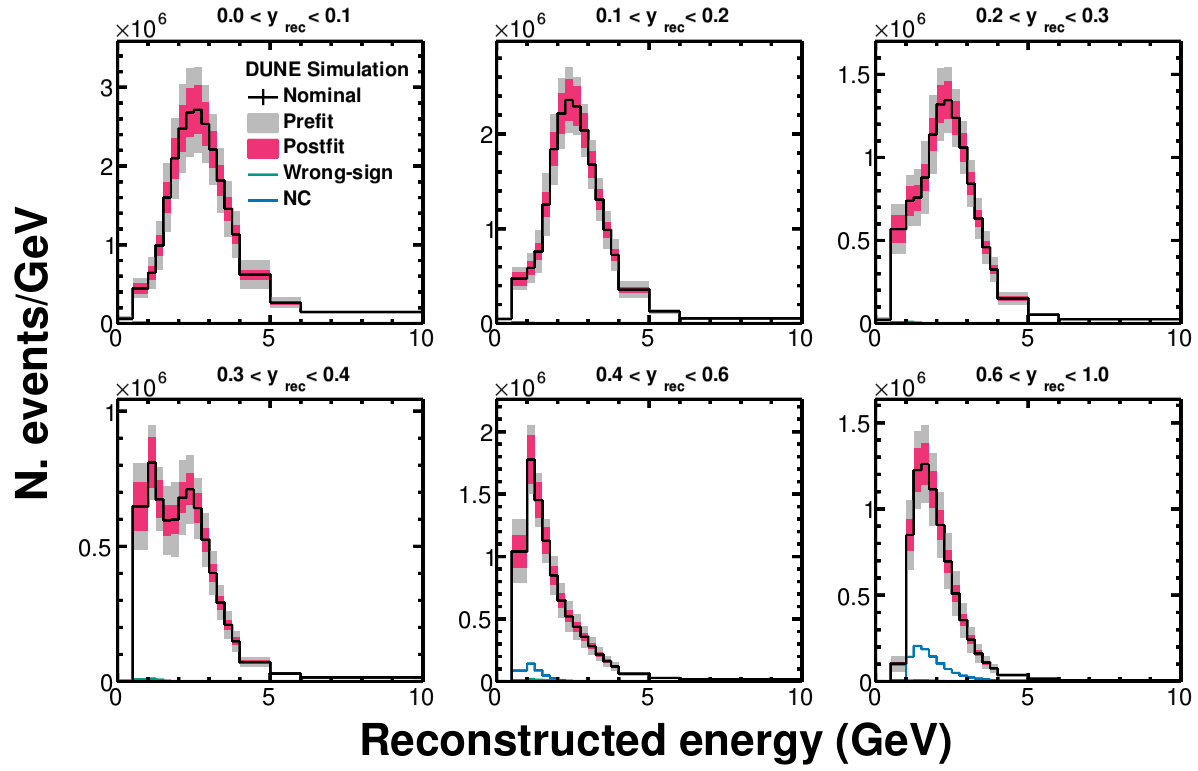
\includegraphics[width=0.8\linewidth]{ND_FHC_ndfd100ktMWyr_allsyst_asimov0_th13_constraint.png}}\\
  \subfloat[RHC]{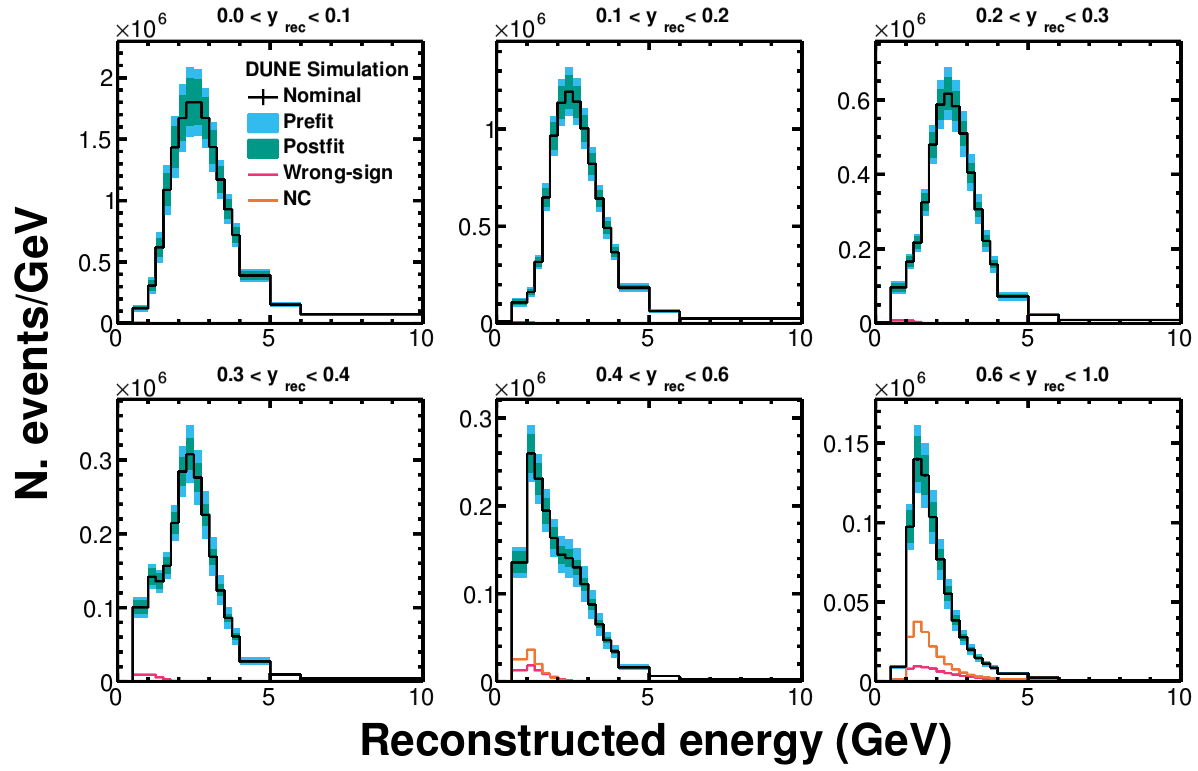
\includegraphics[width=0.8\linewidth]{ND_RHC_ndfd100ktMWyr_allsyst_asimov0_th13_constraint.png}}
  \caption{ND samples in both FHC and RHC, shown in the reconstructed neutrino energy and reconstructed inelasticity binning used in the analysis, shown for a $\sim$105 ton-year exposure (equivalent to a 100 ktMWyr exposure at the FD), with an equal split between FHC and RHC. The size of the systematic uncertainty bands from all of the flux, cross-section and ND detector systematics used in the analysis are shown, as well as the postfit uncertainty bands obtained by performing an Asimov fit to the ND data. Background are also shown, which are dominated by NC events, although there is some contribution from wrong-sign \numu background events in RHC.}
 \label{fig:nd_samples}
\end{figure*}
The oscillation analysis presented here includes samples of $\nu_{\mu}$ and $\bar{\nu}_{\mu}$ charged-current interactions originating in the LAr portion of the ND. These samples are binned in two dimensions as a function of reconstructed neutrino energy and inelasticity, $y_{\mathrm{rec}} = 1 - E^{\mathrm{rec}}_{\mu}/E^{\mathrm{rec}}_{\nu}$, where $E^{\mathrm{rec}}_{\mu}$ and $E^{\mathrm{rec}}_{\nu}$ are the reconstructed muon and neutrino energies, respectively. The sample distributions for both FHC and RHC are shown in Figure~\ref{fig:nd_samples} for an exposure of $\sim$105 ton-years, equivalent to 100 ktMWyr at the far detector with the assumptions stated above. The size of the systematic uncertainty bands from all of the flux, cross-section and ND detector systematics used in the analysis and described above are shown, as well as the postfit uncertainty bands obtained by performing an Asimov fit to the ND data. It is clear that even after a relatively small exposure of 105 ton-years, the ND samples are very high statistics, and are systematics limited in the binning used in the analysis. Backgrounds in the $\nu^{\bracketbar}_{\mu}$-CC samples are also shown in Figure~\ref{fig:nd_samples}: NC backgrounds are predominantly from NC $\pi^{\pm}$ production where the pion leaves a long track and does not shower; wrong-sign contamination in the beam is a background where the charge of the muon is not reconstructed, which particularly affects low reconstructed neutrino energies in RHC.

\begin{figure}[htbp]
 \subfloat[FHC]{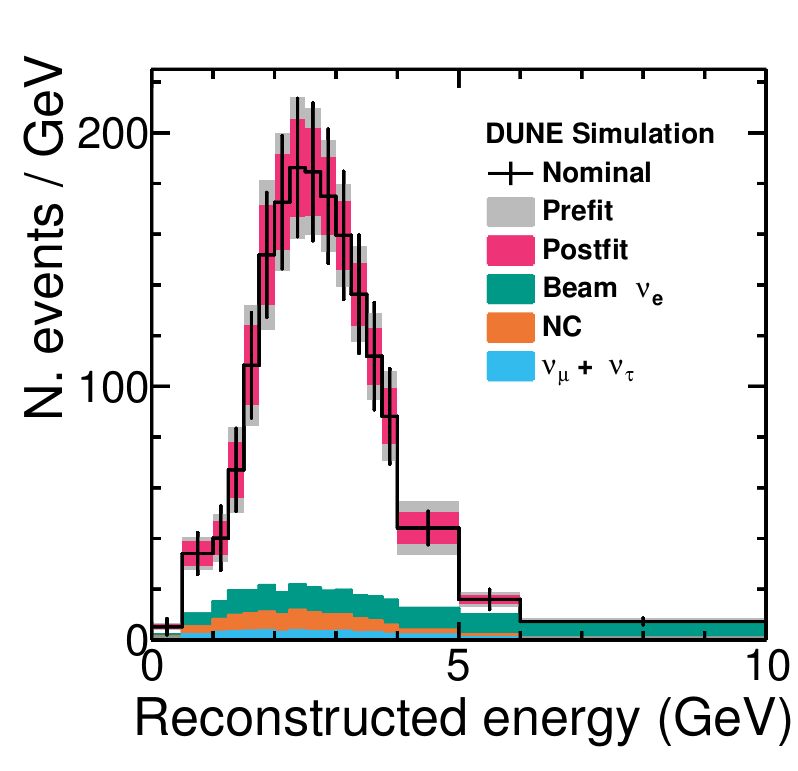
\includegraphics[width=0.8\linewidth]{FD_nue_FHC_ndfd100ktMWyr_allsyst_asimov0_th13_constraint.png}}\\
 \subfloat[RHC]{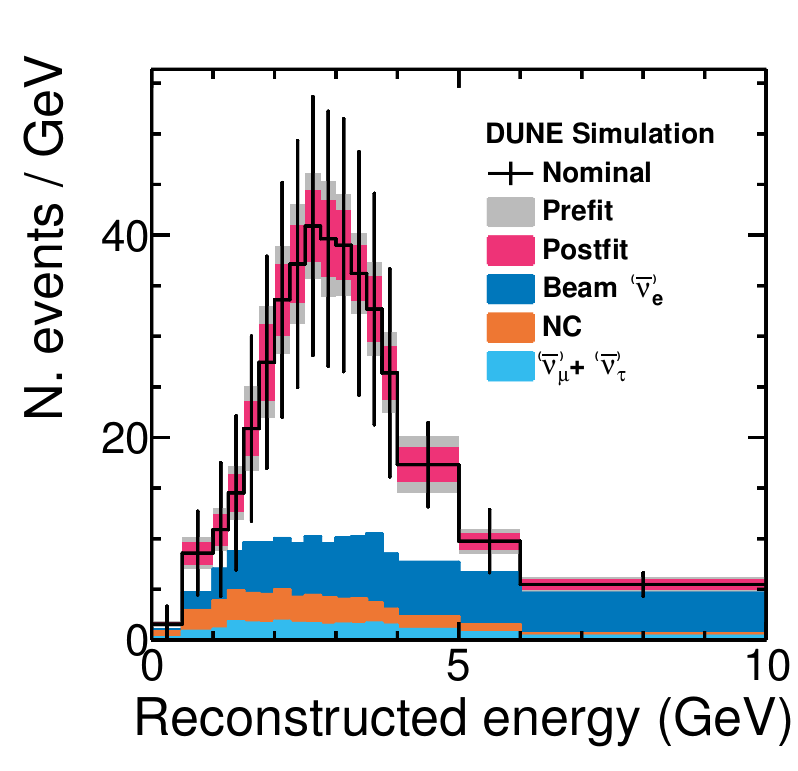
\includegraphics[width=0.8\linewidth]{FD_nue_RHC_ndfd100ktMWyr_allsyst_asimov0_th13_constraint.png}}
 \caption{Reconstructed energy distribution of selected CC $\nue^{\bracketbar}$-like events for a 50 ktMWyr exposure in both neutrino-enhanced FHC beam mode and antineutrino-enhanced RHC beam mode, for a total 100 ktMWyr year exposure. The plots are shown for NO, all other oscillation parameters are set to their NuFIT 4.0 best-fit values (see Table~\ref{tab:oscpar_nufit}). The size of the systematic uncertainty bands from all of the flux, cross-section and FD detector systematics used in the analysis are shown, as well as the postfit uncertainty bands with parameters constrained by ND data. Backgrounds are also shown, the largest contribution comes from intrinsic $\nue^{\bracketbar}$ contamination in the beam, although NC and other flavors, $\numu^{\bracketbar} + \nutau^{\bracketbar}$, also contribute.}
 \label{fig:appspectra}
\end{figure}
The expected FD FHC \nue and RHC \anue samples are shown in Figure~\ref{fig:appspectra} for a 100 ktMWyr total FD exposure, split equally into FHC and RHC beam modes. The systematic uncertainty bands with and without the ND constraint applied are shown, as well as the background contributions. Note that there are contributions from both \nue and \anue in both beam modes. The NC, intrinsic beam $\nue^{\bracketbar}$, and wrong flavor contamination is also shown, the largest background comes from the intrinsic $\nue^{bracketbar}$ beam contribution in both modes. After a 50 ktMWyr exposure in FHC, the \nue sample statistical uncertainty is close to the systematic uncertainty before the ND constraint, although is still clearly statistics limited when the ND constraint is applied. The \anue sample is still strongly statistics limited after 50 ktMWyr exposure in RHC. The difference is largely due to the difference in the \nue and \anue cross sections. The $\nue^{\bracketbar}$ samples in both modes are clearly statistics limited until much larger exposures.

\begin{figure}[htbp]
  \subfloat[FHC]{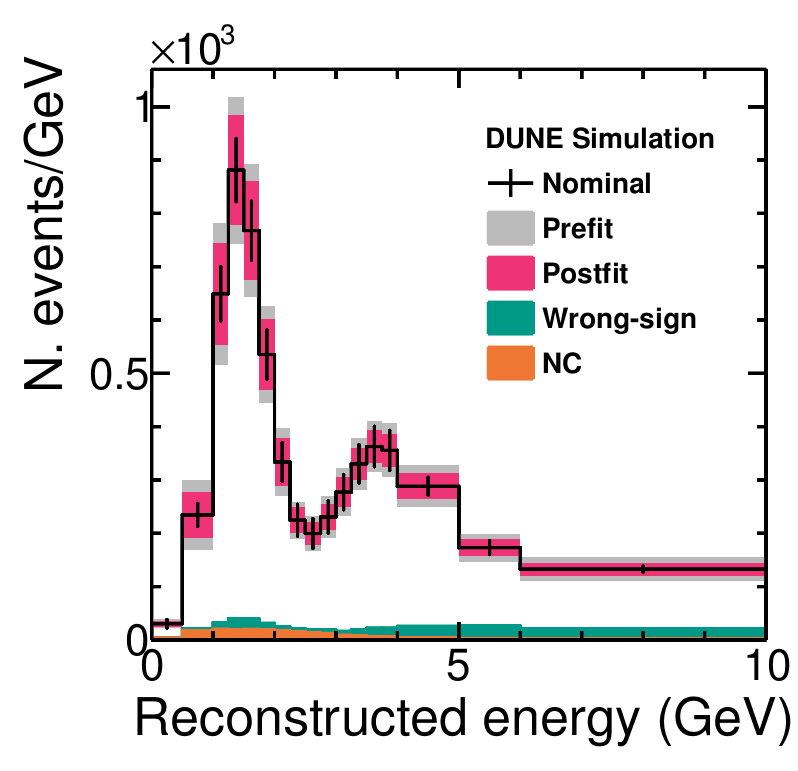
\includegraphics[width=0.8\linewidth]{FD_numu_FHC_ndfd100ktMWyr_allsyst_asimov0_th13_constraint.png}}\\
  \subfloat[RHC]{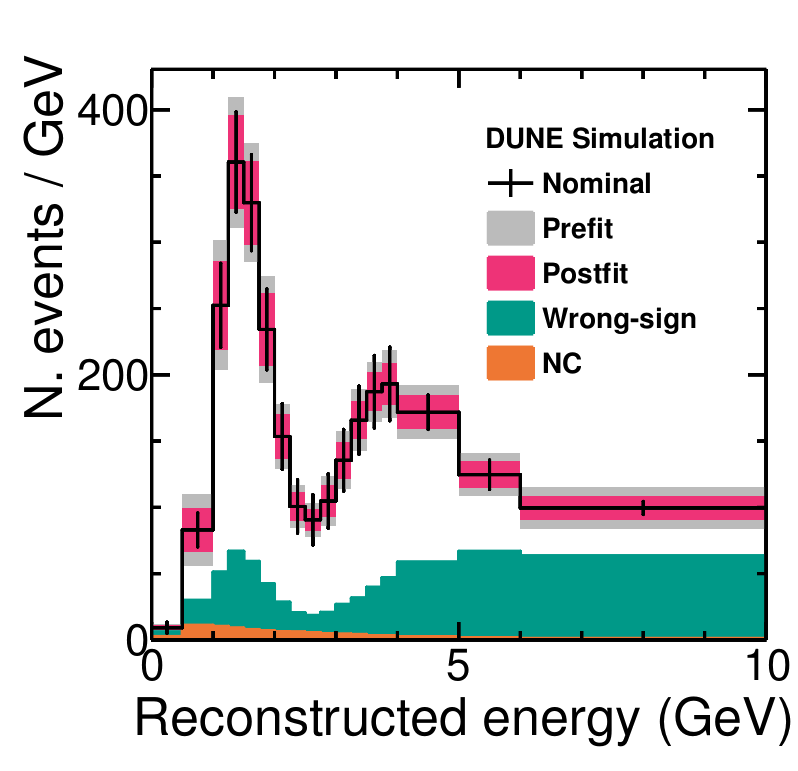
\includegraphics[width=0.8\linewidth]{FD_numu_RHC_ndfd100ktMWyr_allsyst_asimov0_th13_constraint.png}}
\caption{Reconstructed energy distribution of selected CC $\nu^{\bracketbar}_{\mu}$-like events for 50 ktMWyr exposure in both neutrino-enhanced FHC beam mode and antineutrino-enhanced RHC beam mode, for a total 100 ktMWyr year exposure. The plots are shown for NO, all other oscillation parameters are set to their NuFIT 4.0 best-fit values (see Table~\ref{tab:oscpar_nufit}). The size of the systematic uncertainty bands from all of the flux, cross-section and ND detector systematics used in the analysis are shown, as well as the postfit uncertainty bands with parameters constrained by ND data. NC and wrong-sign backgrounds are also shown, the only sizeable background is the wrong-sign (\numu) contribution to the RHC same.}
\label{fig:disspectra}
\end{figure}
The expected FD FHC \numu and RHC \anumu samples are shown in Figure~\ref{fig:disspectra} for a 100 ktMWyr total FD exposure, split equally into FHC and RHC beam modes. The systematic uncertainty bands with and without the ND constraint applied are shown, as well as the background contributions. Note that although the wrong-sign \numu contribution to the RHC \anumu sample is identified as a background, it still provides useful information, it just complicates the analysis. The statistics are much higher than in Figure~\ref{fig:appspectra}, the statistical uncertainty on the \numu FHC sample is smaller than the systematic uncertainty band for some regions of phase space, even after the ND constraint is applied, although the statistical uncertainty is larger than the constrained systematic uncertainty in the ``dip'' region, around 2.5 GeV, which is likely to have the most impact on the analysis. The statistical uncertainty on the \anumu RHC sample is larger, again due to the smaller \anumu than \numu cross section, and the statistical uncertainty around the 2.5 GeV dip region is significantly larger than the systematic uncertainty band, although as for the FHC \numu sample, the statistical uncertainty is smaller than the systematics for some regions of the parameter space.

Note that the events with reconstructed neutrino energy less than 0.5 GeV (which are shown in Figures~\ref{fig:appspectra} and~\ref{fig:disspectra}) or neutrino energies greater than 10 GeV are not included in the analysis for any of the FD or ND samples.




% \input{sections/flux}
% \input{sections/nuint}
% \input{sections/nd}
% \input{sections/fd}
\section{Expected Far Detector Event Rate and Oscillation Parameters}
\label{sec:rate}

In this work, FD event rates are calculated assuming the following nominal deployment plan, which is based on a technically limited schedule:
\begin{itemize}
    \item Start of beam run: two FD module
    volumes for total fiducial mass of 20 kt, 1.2 MW beam
    \item After one year: add one FD module  volume for total fiducial mass of 30 kt
    \item After three years: add one FD module  volume for total fiducial mass of 40 kt
    \item After six years: upgrade to 2.4 MW beam
\end{itemize}
Table~\ref{tab:exposures} shows the conversion between number of years under the nominal staging plan, and  kt-MW-years, which are used to indicate the exposure in this analysis. For all studies shown in this work, a 50\%/50\% ratio of FHC to RHC data was assumed, based on studies which showed a roughly equal mix of running produced a nearly optimal \deltacp and mass ordering sensitivity. The exact details of the run plan are not included in the staging plan.

\begin{table}[htbp]
  \centering
  \begin{tabular}{cc}
    \hline
    Years & kt-MW-years \\
    \hline\hline
    7 & 336 \\
    10 & 624 \\
    15 & 1104 \\
    \hline
  \end{tabular}
  \caption{Conversion between number of years in the nominal staging plan, and kt-MW-years, the two quantities used to indicate exposure in this analysis.}
  \label{tab:exposures}
\end{table}

Event rates are calculated with the assumption of 1.1 $\times 10^{21}$ POT per year, which assumes a combined uptime and efficiency of the FNAL accelerator complex and the LBNF beamline of 57\%~\cite{Abi:2020evt}.

% \input{sections/syst}
% \input{sections/methods}
\section{Run plan optimization}
\label{sec:run_plan_opt}
In previous DUNE sensitivity studies~\cite{Abi:2020qib}, equal running times in FHC and RHC were assumed, based on early sensitivity estimates for different scenarios. In this section, the dependence of the median CPV and mass ordering significances are studied, for different fractions of time spent in each beam mode, using the full analysis framework described in Section~\ref{sec:analysis_framework}.
\begin{figure*}[htbp]
  \centering
  \subfloat[NO, with $\theta_{13}$-penalty] {\includegraphics[width=0.4\linewidth]{{cpv_sens_ndfd100kTMWyr_th13_asimov0_nh}.png}}
  \subfloat[IO, with $\theta_{13}$-penalty] {\includegraphics[width=0.4\linewidth]{{cpv_sens_ndfd100kTMWyr_th13_asimov0_ih}.png}}\\
  \subfloat[NO, no $\theta_{13}$-penalty]   {\includegraphics[width=0.4\linewidth]{{cpv_sens_ndfd100kTMWyr_nopen_asimov0_nh}.png}}
  \subfloat[IO, no $\theta_{13}$-penalty]   {\includegraphics[width=0.4\linewidth]{{cpv_sens_ndfd100kTMWyr_nopen_asimov0_ih}.png}}
  \caption{The Asimov CPV sensitivity as a function of the true value of \deltacp, for a total exposure of 100 kt-MW-yrs with different fractions of FHC and RHC running, with and without a $\theta_{13}$ penalty applied in the fit. Results are shown for both true normal and inverted ordering, with the true oscillation parameter values set to the NuFit 4.0 best fit point in each ordering (see Table~\ref{tab:oscpar_nufit}).}
  \label{fig:run_opt_cpv}
\end{figure*}

Figure~\ref{fig:run_opt_cpv} shows DUNE's Asimov sensitivity to CPV for a total 100 kt-MW-yrs far detector exposure, with different fractions of FHC and RHC running, at the NuFIT 4.0 best fit value in both NO and IO (see Table~\ref{tab:oscpar_nufit}), shown with and without a penalty on $\theta_{13}$ applied. For each point tested, all oscillation and nuisance parameters are allowed to vary, and two fits are carried out, one where \deltacp is only allowed to take CP-conserving values, and another where it is allowed to vary. The difference in the best-fit $\chi^{2}$ values is calculated:
\begin{equation}
  \Delta\chi^{2} = \min\left\{\chi^{2}_{\deltacp = -\pi},\chi^{2}_{\deltacp = 0},\chi^{2}_{\deltacp = \pi}\right\} - \chi^{2}_{\mathrm{CPV}},
  \label{eq:cpv_chi2}
\end{equation}
\noindent and the square root of the difference is  used as the figure of merit on the y-axis in Figure~\ref{fig:run_opt_mh}. We note that there are some caveats associated with this figure of merit, which are discussed in Section~\ref{sec:cp_sens}. A 100 kt-MW-yrs exposure is shown as it was identified in Ref~\cite{Abi:2020qib} as the exposure at which DUNE's median CPV significance exceeds 3$\sigma$ at $\deltacp = \pm\pi/2$, an important milestone in DUNE's physics program (with equal beam mode running). 

%\chris{I find this paragraph jargony, i.e. terms like ``th13 penalty'' and ``octant degeneracy'' could be explained a bit more.  I have attempted a rewrite below.}
%Figure~\ref{fig:run_opt_cpv} shows that with a $\theta_{13}$ applied, the sensitivity to CPV can be increased in some regions of \deltacp parameter space with more FHC than RHC running. However this degrades the sensitivity in other regions, most notably for $\deltacp > 0$ regardless of the true mass ordering, where the octant degeneracy starts to strongly impact the results. For regions of phase space where the octant degeneracy does not affect the result (e.g., $\sin^{2}\theta_{23} \approx 0.5$), there is no degredation in the sensitivity, and enhanced FHC running increases the sensitivity for all values of \deltacp. Increasing the fraction of RHC decreases the sensitivity for the entire \deltacp range when the $\theta_{13}$ penalty is applied, relative to equal beam mode running, which can be understood as being due to the lower statistics of the \anue sample (see Figure~\ref{fig:appspectra}). Although for low exposures, DUNE will not have a strong constraint on $\theta_{13}$, so the main analysis will include a $\theta_{13}$ penalty, it is instructive to look at the results without the penalty applied. In the no penalty case, the sensitivity is severely degraded (as expected) for 100\% running in either beam mode.

Figure~\ref{fig:run_opt_cpv} shows that when the reactor constraint on $\theta_{13}$ is included, the sensitivity to CPV can be increased in some regions of \deltacp parameter space with more FHC than RHC running. However, this degrades the sensitivity in other regions, most notably for $\deltacp > 0$ regardless of the true mass ordering. This is due to a degeneracy between \deltacp and the octant of $\sinstt{23}$ because both parameters impact the rate of \nue appearance. The degeneracy is resolved by including antineutrino data; the octant of $\sinstt{23}$ affects the rate of \nue and \anue appearance in the same way, but the effect of \deltacp is reversed for antineutrinos.

For regions of phase space where the octant degeneracy does not affect the result (e.g., $\sin^{2}\theta_{23} \approx 0.5$), there is no degredation in the sensitivity, and enhanced FHC running increases the sensitivity for all values of \deltacp. Increasing the fraction of RHC decreases the sensitivity for the entire \deltacp range when the reactor $\theta_{13}$ constraint is included, relative to equal beam mode running. This is due to the lower statistics of the \anue sample (see Figure~\ref{fig:appspectra}) because of the reduced antineutrino flux and cross section. For short exposures, DUNE will not have a competitive independent measurement of $\theta_{13}$, so the main analysis will include the reactor $\theta_{13}$ constraint. Nonetheless, it is instructive to look at the results without the penalty applied. In this case, the sensitivity is severely degraded (as expected) for 100\% running in either beam mode.


\begin{figure*}[htbp]
  \centering
  \subfloat[NO, with $\theta_{13}$-penalty]  {\includegraphics[width=0.4\linewidth]{{mh_sens_ndfd24kTMWyr_th13_asimov0_nh}.png}}
  \subfloat[IO, with $\theta_{13}$-penalty]  {\includegraphics[width=0.4\linewidth]{{mh_sens_ndfd24kTMWyr_th13_asimov0_ih}.png}}\\
  \subfloat[NO, no $\theta_{13}$-penalty]    {\includegraphics[width=0.4\linewidth]{{mh_sens_ndfd24kTMWyr_nopen_asimov0_nh}.png}}
  \subfloat[IO, no $\theta_{13}$-penalty]    {\includegraphics[width=0.4\linewidth]{{mh_sens_ndfd24kTMWyr_nopen_asimov0_ih}.png}}
  \caption{The Asimov mass ordering sensitivity as a function of the true value of \deltacp, for a total exposure of 24 kt-MW-yrs with different fractions of FHC and RHC running, with and without a $\theta_{13}$ penalty applied in the fit. Results are shown for both true normal and inverted ordering, with the true oscillation parameter values set to the NuFIT 4.0 best fit point in each ordering (see Table~\ref{tab:oscpar_nufit}).}
  \label{fig:run_opt_mh}
\end{figure*}
Figure~\ref{fig:run_opt_mh} shows DUNE's Asimov sensitivity to the mass ordering for a total 24 kt-MW-yrs far detector exposure, with different fractions of FHC and RHC running, and the same four true oscillation parameter sets. For each point tested, all oscillation and nuisance parameters are allowed to vary, and two fits are carried out, one using each ordering. The difference in the best-fit $\chi^{2}$ values is calculated:
\begin{equation}
  \Delta\chi^{2} = \chi^{2}_{\mathrm{IO}} - \chi^{2}_{\mathrm{NO}},
  \label{eq:mh_chi2}
\end{equation}
\noindent and the square root of the difference is used as the figure of merit on the y-axis in Figure~\ref{fig:run_opt_mh}. We note that there are some caveats associated with this figure of merit, which are discussed in Section~\ref{sec:mh_sens}. A 24 kt-MW-yrs exposure is used in Figure~\ref{fig:run_opt_mh} as it is around the exposure at which DUNE's median mass ordering significance exceeds 5$\sigma$ for some vales of \deltacp~\cite{Abi:2020qib}.

It is clear from Figure~\ref{fig:run_opt_mh} that the mass ordering sensitivity has a strong dependence on the fraction of running in each beam mode. As in the CPV case, the effect is very different with and without the reactor $\theta_{13}$ constraint included. If the true ordering is normal and the reactor $\theta_{13}$ penalty is applied, the sensitivity increases significantly with increasing FHC running, with a full 1$\sigma$ increase in the sensitivity between equal beam running and 100\% FHC for most values of \deltacp. Conversely, if the ordering is inverted, 100\% FHC running would degrade the sensitivity by $\geq$1$\sigma$ for all values of \deltacp at the NuFIT 4.0 best fit point. Overall the sensitivity to the inverted ordering is improved by a more equal split between the beam modes. It is clear that 100\% RHC running gives poor sensitivity for all values tested. 

Without the reactor $\theta_{13}$ constraint, the greatest sensitivity is obtained with close to an equal split of FHC and RHC running, and the sensitivity is significantly reduced with 100\% FHC running. This is because of a degeneracy between the effect of $\theta_{13}$ and the mass ordering on the rate of \nue appearance in FHC mode. If the mass ordering is normal, the \nue rate in FHC will be enhanced; without the reactor constraint, this excess can be accommodated by increasing the value of $\theta_{13}$.

\begin{figure*}[htbp]
  \centering
  \subfloat[CPV, with $\theta_{13}$-penalty] {\includegraphics[width=0.4\linewidth]{{cpv_sens_ndfd334kTMWyr_th13_asimov0_nh}.png}}
  \subfloat[CPV, no $\theta_{13}$-penalty]   {\includegraphics[width=0.4\linewidth]{{cpv_sens_ndfd334kTMWyr_nopen_asimov0_nh}.png}}\\
  \subfloat[MO, with $\theta_{13}$-penalty]  {\includegraphics[width=0.4\linewidth]{{mh_sens_ndfd334kTMWyr_th13_asimov0_nh}.png}}
  \subfloat[MO, no $\theta_{13}$-penalty]    {\includegraphics[width=0.4\linewidth]{{mh_sens_ndfd334kTMWyr_nopen_asimov0_nh}.png}}
  \caption{The Asimov CPV and mass ordering sensitivities as a function of the true value of \deltacp, for a total exposure of 334 kt-MW-yrs with different fractions of FHC and RHC running, with and without a $\theta_{13}$ penalty applied in the fit. Results are shown for both true normal ordering only, with the true oscillation parameter values set to the NuFIT 4.0 NO best fit point (see Table~\ref{tab:oscpar_nufit}).}
  \label{fig:run_opt_334ktmwyr}
\end{figure*}

For comparison, Figure~\ref{fig:run_opt_334ktmwyr} shows the Asimov CPV and mass ordering sensitivities, with and without the reactor $\theta_{13}$ constraint included, for true normal ordering only, for a large exposure of 334 kt-MW-yrs, with different fractions of FHC and RHC running. At large exposures, running with strongly enhanced FHC running no longer improves the sensitivity over equal beam mode running, with or without the $\theta_{13}$ penalty applied, for either CPV or mass ordering determination. 

Overall, the sensitivity to CPV and the mass ordering is dependent on the division of running time between FHC and RHC, but a choice that increases the sensitivity in some region of parameter space can severely decrease the sensitivity in other regions. If there is strong reason to favor, for example, normal over inverted ordering when DUNE starts to take data, Figure~\ref{fig:run_opt_mh} shows that this could be more rapidly verified by running with more FHC data than RHC data, as the reactor $\theta_{13}$ constraint will be used in the main low exposure analysis. However, if this choice is wrong, this might cause DUNE to take longer to reach the same significance. Clearly this is an important consideration which should be revisited shortly before DUNE begins to collect data. Similarly, the CPV sensitivity shown in Figure~\ref{fig:run_opt_cpv} might be optimized if there is a strong reason to favor gaining sensitivity for $\deltacp > 0$ or $\deltacp < 0$, at a cost of reducing the sensitivity to CPV if \deltacp has the other sign. But, it is clear from Figures~\ref{fig:run_opt_cpv} and~\ref{fig:run_opt_mh} that equal running in FHC and RHC gives a close to optimal sensitivity across all of the parameter space, and as such is a reasonable {\it a priori} choice of run plan for studies of the DUNE sensitivity. Additionally, it is clear from Figure~\ref{fig:run_opt_334ktmwyr} that the improvement in the sensitivity with unequal beam running is a feature at low exposures, but not at high exposures, particularly because at high exposures when DUNE is able to constrain all the oscillation parameters with precision~\cite{Abi:2020qib}, there is a stronger motivation to run a DUNE-only analysis, without relying on the reactor $\theta_{13}$ measurement.



\FloatBarrier
\section{CP violation sensitivity}
\label{sec:cp_sens}

In this section, CPV sensitivity results are presented. For simplicity, only true NO will be shown unless explicitly stated. In all cases, a joint ND+FD fit is performed, and a $\theta_{13}$ penalty is always applied, as described in Section~\ref{sec:analysis_framework}. An equal split between FHC and RHC running is assumed based on the results obtained in Section~\ref{sec:run_plan_opt}. The Asimov sensitivities as shown in Section~\ref{sec:run_plan_opt} are informative, but do not give information on how the expected sensitivity may vary with statistical or systematic uncertainties. Or for variations in the other oscillation parameters of interest.

\begin{figure}[htbp]
  \centering
  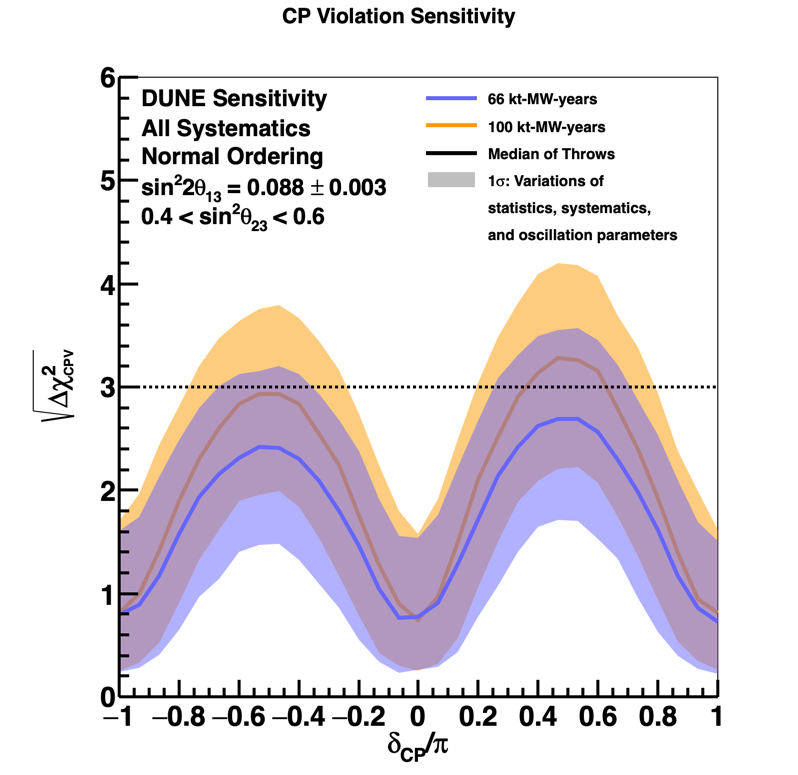
\includegraphics[width=0.8\linewidth, trim={0cm 0cm 0cm 2.3cm}, clip]{cpv_two_exps_throws_nh_2019_v4_lowexp.png}\\
  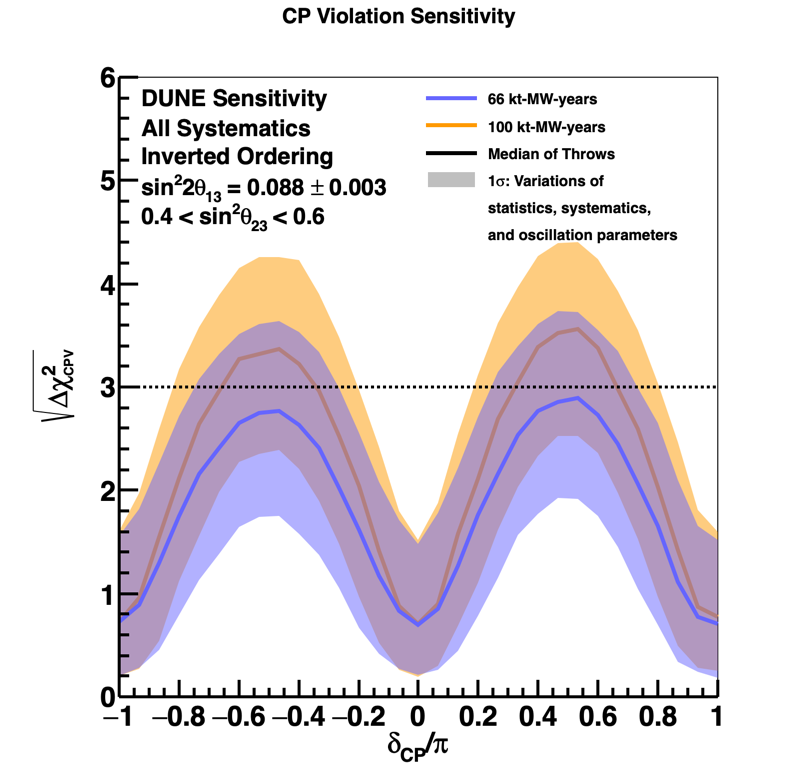
\includegraphics[width=0.8\linewidth, trim={0cm 0cm 0cm 2.3cm}, clip]{cpv_two_exps_throws_ih_2019_v4_lowexp.png}
  \caption{Significance of the DUNE determination of CP-violation ($\deltacp \neq [0,\pm\pi]$) as a function of the true value of \deltacp, for 66 ktMWyr (blue) and 100 ktMWyr (orange) exposures, for normal (top) and inverted (bottom) orderings. The width of the transparent bands cover 68\% of fits in which random throws are used to simulate systematic, oscillation parameter and statistical variations, with independent fits performed for each throw constrained by pre-fit uncertainties. The solid lines show the median sensitivity.}
  \label{fig:cpv_bands}
\end{figure}
Figure~\ref{fig:cpv_bands} shows the significance with which CPV ($\deltacp \neq [0, \pm\pi]$) can be observed for both NO and IO, for exposures of 66 kTMWyr and 100 ktMWyr. For each throw of the systematic, other oscillation parameters and statistics, two fits are carried out, one where the \deltacp is fixed at CP-conserving values, and another where it is allowed to vary. The difference in the best-fit $\chi^{2}$ values is calculated:
\begin{equation}
  \Delta\chi^{2} = \chi^{2}_{0,\pm\pi} - \chi^{2}_{\mathrm{CPV}},
  \label{eq:cpv_chi2}
\end{equation}
\noindent and the square root of the difference is the significance shown on the y-axis of Figure~\ref{fig:cpv_bands}. We note that this constant-\dchisq method is valid as long as Wilks' can be applied~\cite{wilks}.

The sensitivity shown in Figure~\ref{fig:cpv_bands} has the characteristic double peak structure because the significance of a CPV measurement decreases around CP-conserving values. The median sensitivity never reaches exactly zero at CP-conserving values due to the systematic and statistical throws. Median sensitivities are slightly higher for IO than for NO, and by exposures of 100 ktMWyr, the median sensitivity exceeds 3$\sigma$ for the maximal CP-violating values of $\pm\pi/2$. This presentation of the CPV sensitivity was followed in Ref.~\cite{Abi:2020qib}, and is very informative at high exposures. However at low exposures as shown in Figure~\ref{fig:cpv_bands}, the spread in the sensitivity is harder to interpret.

\begin{figure*}[htbp]
  \centering
  \subfloat[24 ktMWyr] {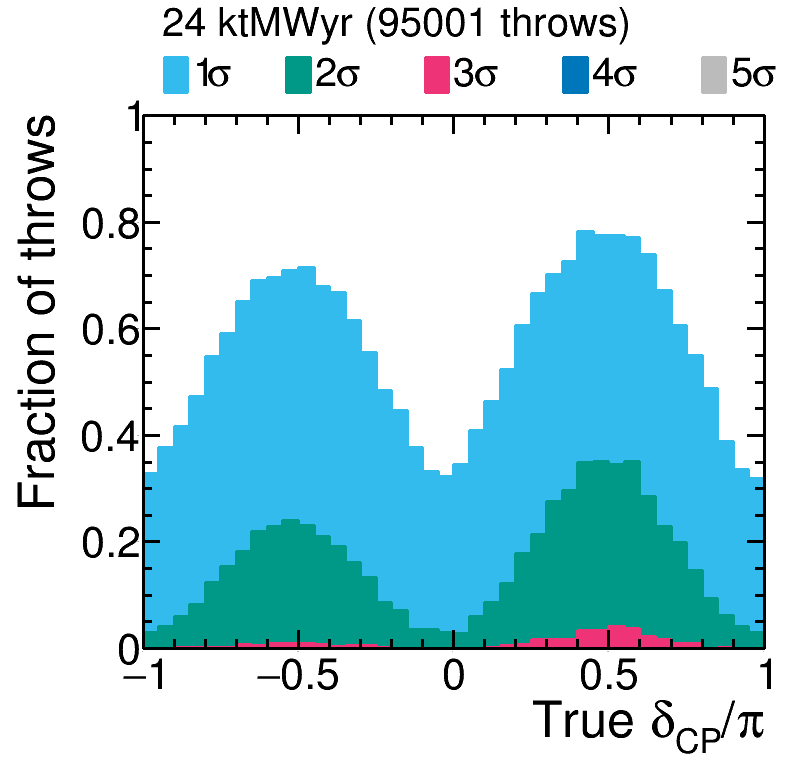
\includegraphics[width=0.33\linewidth]{cpv_throws_24ktMWyr_NH_th13.png}}
  \subfloat[66 ktMWyr] {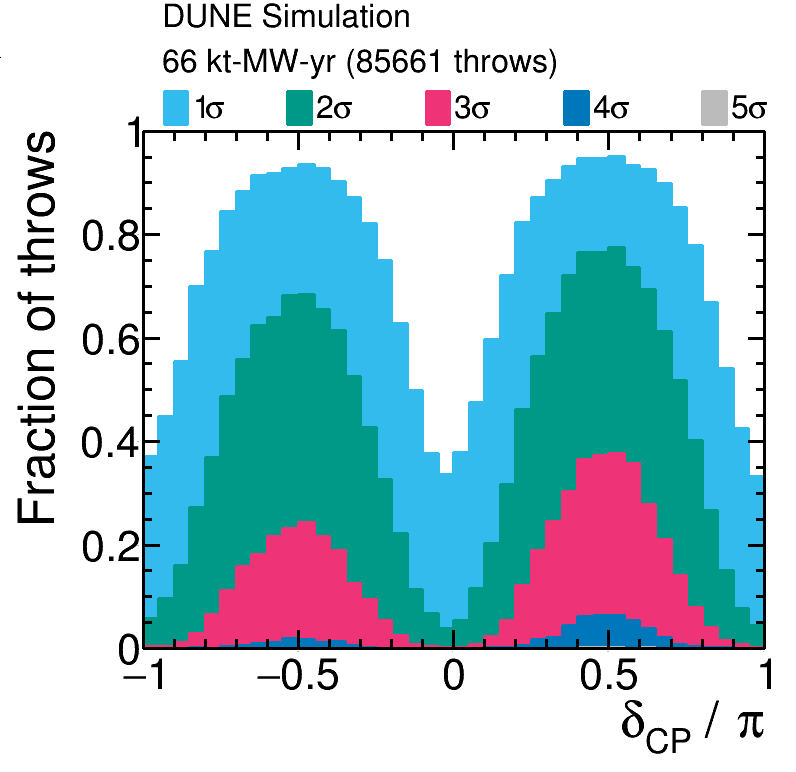
\includegraphics[width=0.33\linewidth]{cpv_throws_66ktMWyr_NH_th13.png}}
  \subfloat[100 ktMWyr]{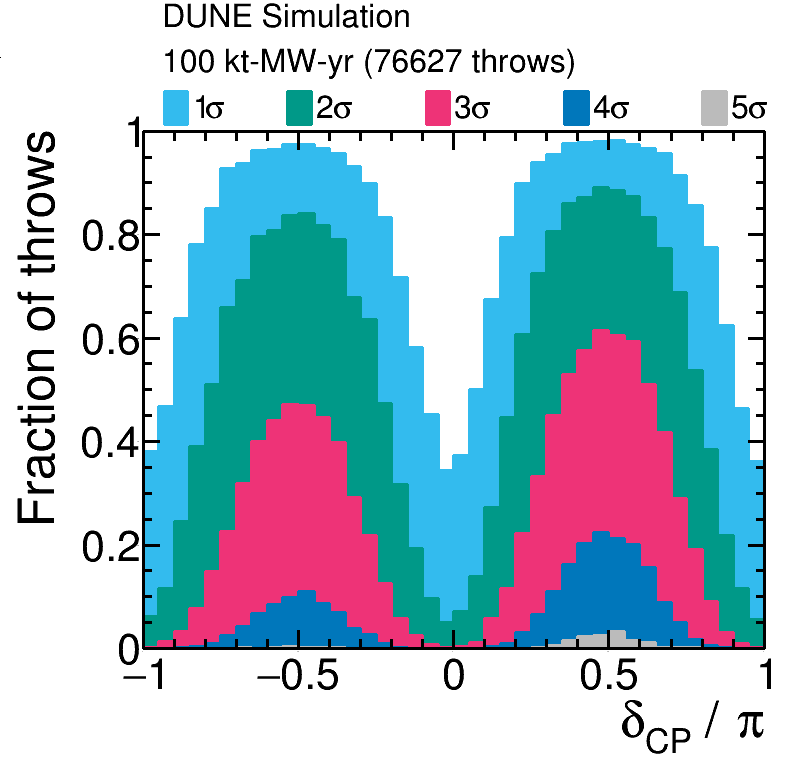
\includegraphics[width=0.33\linewidth]{cpv_throws_100ktMWyr_NH_th13.png}}\\
  \subfloat[150 ktMWyr]{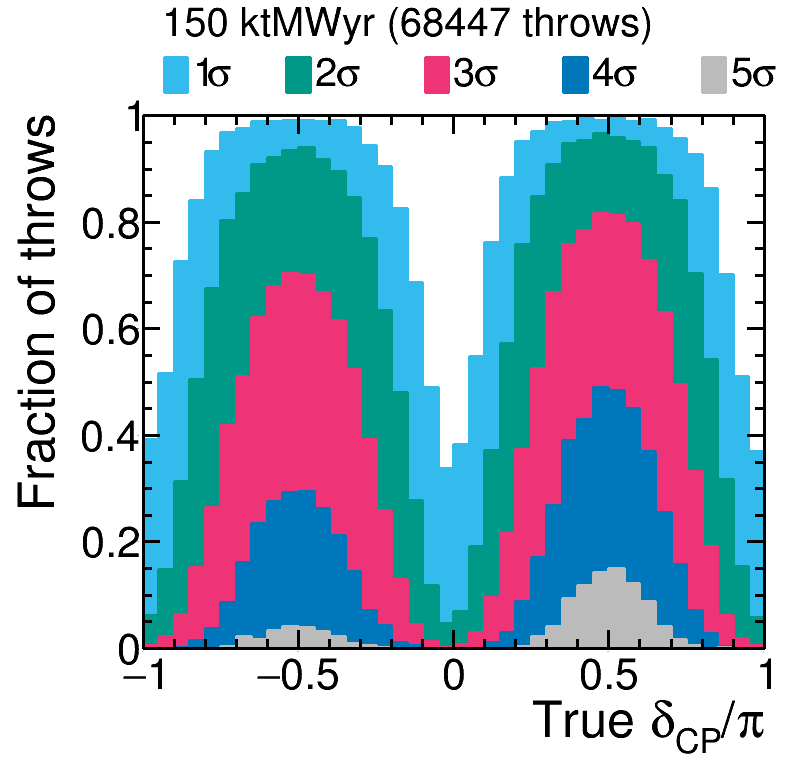
\includegraphics[width=0.33\linewidth]{cpv_throws_150ktMWyr_NH_th13.png}}
  \subfloat[197 ktMWyr]{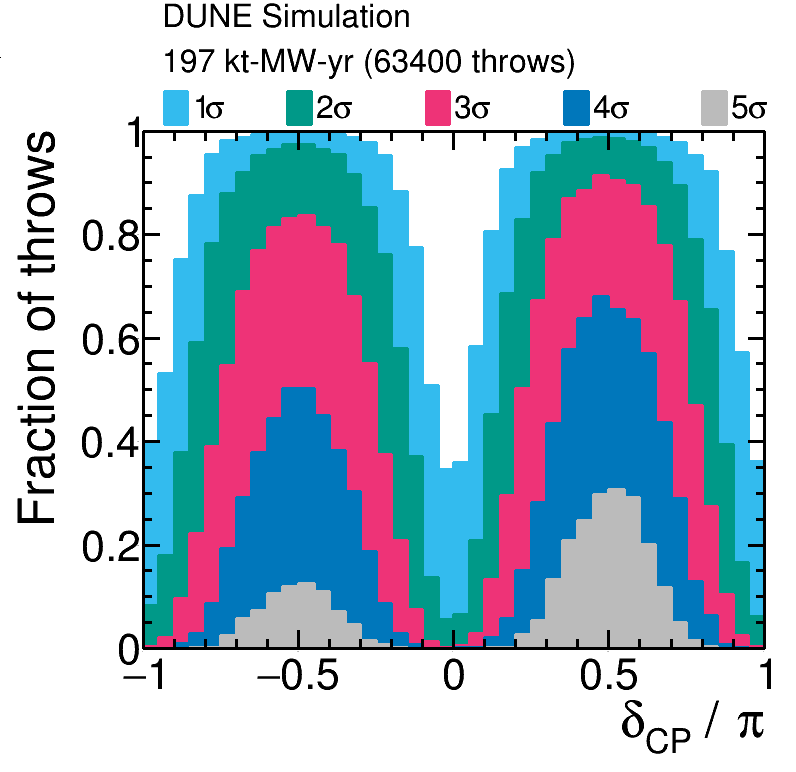
\includegraphics[width=0.33\linewidth]{cpv_throws_197ktMWyr_NH_th13.png}}
  \subfloat[334 ktMWyr]{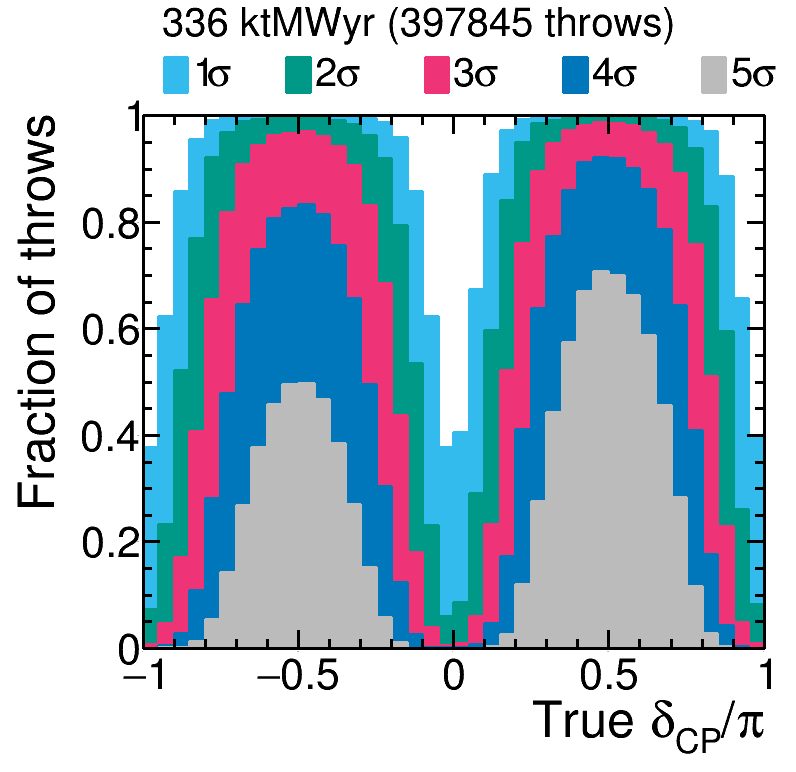
\includegraphics[width=0.33\linewidth]{cpv_throws_334ktMWyr_NH_th13.png}}
  \caption{Fraction of throws for which the DUNE sensitivity to CP-violation ($\deltacp \neq [0,\pm\pi]$) exceeds 1--5$\sigma$ significance, as a function of the true value of \deltacp. Shown for NO, for a number of different exposures. The number of throws used to make each figure is also shown.}
  \label{fig:cpv_over_time}
\end{figure*}
\begin{figure*}[htbp]
  \centering
  \subfloat[$\deltacp = -\pi/2$] {\includegraphics[width=0.8\columnwidth]{{fraction_throws_vs_exp_dcp-0.5}.pdf}}
  \subfloat[$\deltacp = +\pi/2$] {\includegraphics[width=0.8\columnwidth]{{fraction_throws_vs_exp_dcp0.5}.pdf}}
  \caption{Fraction of throws for which the DUNE sensitivity to CP-violation ($\deltacp \neq [0,\pm\pi]$) exceeds 1--5$\sigma$ significance, at $\deltacp = \pm\pi/2$, shown as a function of exposure, for NO.}
  \label{fig:cpv_vs_exp}
\end{figure*}
Figure~\ref{fig:cpv_over_time} provides an alternative way to present the results of the throws. The fraction of throws for which Equation~\ref{eq:cpv_chi2} exceeds different confidence values are shown, for 1--5$\sigma$ significances, for a variety of exposures. It shows the probability for DUNE to observe a significance above a discrete threshold, as a function of the true value of \deltacp. The point at which the median sensitivity (50\% of throws) passes different significance thresholds can be easily read from the figures, and can be compared with those shown in Figure~\ref{fig:cpv_bands}. Note that the highest exposure shown, 334 ktMWyr, is equivalent to the seven year exposure using the staging scenario from Ref.~\cite{Abi:2020qib}. The same double peak structure seen in Figure~\ref{fig:cpv_bands} can be observed. The median sensitivity to CPV exceeds 3$\sigma$ after $\sim$100 ktMWyr, but a significant fraction of throws exceed 3$\sigma$ at 66 ktMWyr. Likewise, although the median significance to CPV does not exceed 5$\sigma$ until $\sim$334 ktMWyr, there are significant fractions of throws at lower exposures which reach $5\sigma$ significance. This presentation also shows that by 334 ktMWyr exposures, the number of throws for which the significance is less than 3$\sigma$ at maximal values of \deltacp is very low. The number of throws used to generate the plots at each exposure is indicated on each plot. The number of throws decreases as a function of exposure because fixed computing resources were used for each configuration, and the time for the ensemble of fits carried out for each throw to complete increases slightly with exposure. The final 334 ktMWyr exposure has more throws because it was generated for the analysis presented in Ref.~\cite{Abi:2020qib}, where more than one projection was considered --- requiring more throws to sample the space.

Figure~\ref{fig:cpv_vs_exp} shows the fraction of throws which exceed different significance thresholds at the maximal \deltacp violation values of $\pm\pi/2$, as a function of exposure. Figure~\ref{fig:cpv_vs_exp} was produced using the same throws used for Figure~\ref{fig:cpv_over_time}, with additional points from higher exposures used in Ref.~\cite{Abi:2020qib}, but not shown in Figure~\ref{fig:cpv_over_time} (646 ktMWyr and 1104 ktMWyr). For NO, the significance at $\deltacp = +\pi/2$ is slightly stronger than at $\deltacp = -\pi/2$. For IO, the significance would be more similar between the two points, which can be observed from Figure~\ref{fig:cpv_bands}, but is not shown in Figures~\ref{fig:cpv_over_time} or~\ref{fig:cpv_vs_exp}.

% \FloatBarrier
% \subsection{Feldman-Cousins studies}
Previous results have been calculated confidence intervals and significances using constant $\Delta\chi^{2}$ critical values. For example, in the CPV results shown in Figure~\ref{fig:cpv_over_time}, the confidence intervals are calculated assuming one degree of freedom, so $\Delta\chi^{2} \leq 1, 4, 9$ corresponds to a significance of 1, 2 and 3$\sigma$. This assumption holds when Wilks' theorem can be applied~\cite{wilks}, but can lead to incorrect coverage where it cannot. This breaks down around physical boundaries, in the case of cyclic parameters, and where there are significant degeneracies. It is likely that a constant $\Delta\chi^{2}$ treatment will break down for \deltacp, where all of these issues apply, as has indeed been shown by T2K~\cite{Abe:2021gky}. The Feldman-Cousins method~\cite{Feldman:1997qc} is a brute force numerical method to calculate confidence intervals with correct coverage.

A large number of toy experiments are produced, where the parameter(s) of interest (here \deltacp) is set to the desired true value, all other systematic and oscillation parameters are thrown, as described in Section~\ref{sec:analysis_framework}, and a statistical throw is made, for the two ND samples and four FD sample used in the analysis. Then two fits are performed, one where the parameter(s) of interest is fixed to the true value, and another where is is allowed to vary. In both fits, all other parameters are allowed to vary. For each throw, a \dchisq is calculated using the minimum $\chi^{2}$ values for those two fits, as in Equation~\ref{dchisq_fc}.
\begin{equation}
  \Delta\chi^{2} = \chi^{2}(\theta_{\mathrm{true}}) - \min_{\theta}\chi^{2}(\theta)
  \label{eq:dchisq_fc}
\end{equation}
\begin{figure}[htbp]
  \centering
  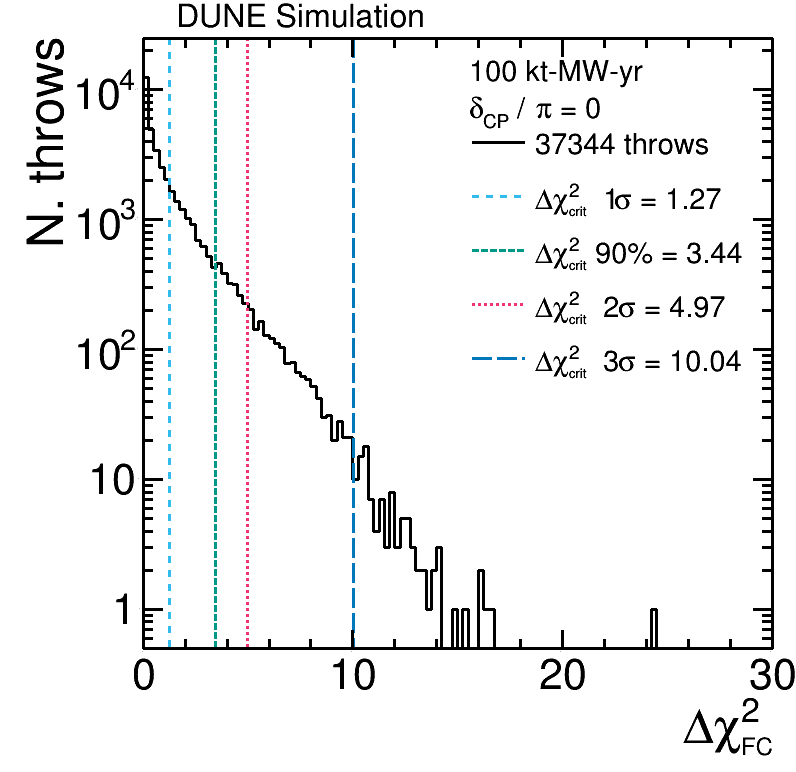
\includegraphics[width=0.8\columnwidth]{nh_FC_ndfd_100ktMWyr_dcp0.png}
  \caption{Distribution of \dchisq values, calculated using Equation~\ref{eq:dchisq_fc}, for a large number of throws with true $\deltacp = 0$, and a 100 ktMWyr exposure. The \dchisqcrit values (vertical lines) obtained using the Feldman-Cousins method show the \dchisq value below which 68.27\% (1$\sigma$), 90\%, 95.45\% (2$\sigma$) and 99.73\% (3$\sigma$) of throws reside, with the calculated values given in the legend. The number of throws used is also given.}
  \label{fig:fc_throws}
\end{figure}
The distribution of these throws is used to calculate the \dchisqcrit that gives the desired coverage, with the appropriate fraction of toys above/below the calculated value. A distribution of \dchisq values is shown in Figure~\ref{fig:fc_throws} for an example ND+FD analysis with a 100ktMWyr exposure at the far detector, equal FHC and RHC run fractions, and with a $\theta_{13}$ penalty applied. In Figure~\ref{fig:fc_throws}, the \dchisqcrit values corresponding to for 68.27\% (1$\sigma$), 90\%, 95.45\% (2$\sigma$) and 99.73\% (3$\sigma$) of the throws are indicated. The \dchisqcrit values were only calculated up to the 3$\sigma$ level due to the very large number of throws required for higher confidence levels.

An uncertainty on the value of \dchisqcrit obtained from the toy throw distribution (e.g., Figure~\ref{fig:fc_throws}), is obtained using a bootstrap rethrowing method~\cite{rice2006mathematical}. The empirical PDF obtained from the throws is treated as the true PDF, and $B$ independent samples of size $n$ are drawn from it, where $n$ is the total number of throws used to build the empirical PDF. Note that each throw can be drawn multiple times in this method. Then, the standard deviation $s_{\hat{\vartheta}}$, on the \dchisqcrit values of interest, $\vartheta$, are calculated for each of the $B$ samples using:
\begin{equation}
  s_{\hat{\vartheta}} = \sqrt{\frac{1}{B} \sum^{B}_{i=0} (\vartheta_{i}^{*} - \bar{\vartheta}^{*})^{2}},
  \label{eq:fc_uncertainty}
\end{equation}
where $\vartheta_{i}^{*}$ denotes the calculated \dchisqcrit value of interest for each of the samples, and $\bar{\vartheta}^{*}$ is their average value.

\begin{figure}[htbp]
  \centering
  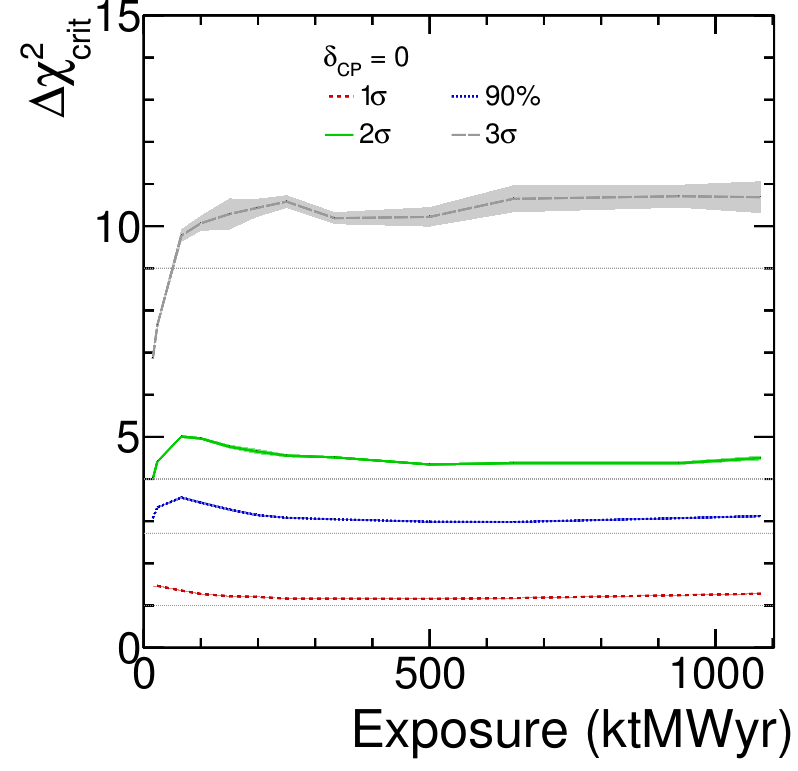
\includegraphics[width=0.8\columnwidth]{dchi2crit_vs_exp_dcp0.png}
  \caption{The \dchisqcrit values corresponding to 68.27\% (1$\sigma$), 90\%, 95.45\% (2$\sigma$) and 99.73\% (3$\sigma$) of throws, shown for true $\deltacp = 0$, as a function of exposure. The uncertainty on the \dchisqcrit values is obtained using Equation~\ref{eq:fc_uncertainty}, and is indicated as the shaded line. To guide the eye, horizontal dashed lines are included which indicate the 1$\sigma$, 90\%, 2$\sigma$ and 3$\sigma$ \dchisq values assumed using the constant-\dchisq method, with one degree of freedom. The distribution of throws used produced to calculate the \dchisqcrit values shown are given in Figure~\ref{fig:fc_throws_exp}.}
  \label{fig:fc_vs_exp}
\end{figure}
Figure~\ref{fig:fc_vs_exp} shows the evolution of the \dchisqcrit values as a function of exposure for $\deltacp = 0$, the relevant value for CPV sensitivity, for an ND+FD analysis with an equal FHC:RHC run fraction and a $\theta_{13}$ penalty applied. Several values were checked for $\deltacp = \pm\pi/2$ and similar results were found. The \dchisqcrit values for all significance levels tested rises quickly and stabilizes at slightly higher than than those suggested by the constant \dchisq method by exposures of $\sim$100 ktMWyr. The initial rise in the \dchisqcrit values is likely to be due to the low statistics at those exposures. Overall, this implies that the CPV significance is probably slightly weaker than assumed in, for example, Figures~\ref{fig:cpv_over_time} and~\ref{fig:cpv_vs_exp}, but not by a great deal. Crucially, there is no constant increase in the \dchisqcrit values over time as has been reported by T2K~\cite{Abe:2021gky}. Details on the number of toy throws used at each point of Figure~\ref{fig:fc_vs_exp} are given in Appendix~\ref{sec:fc_appendix}, and the toy throw distributions are shown in Figure~\ref{fig:fc_throws_exp}.

\begin{figure}[htbp]
  \centering
  \subfloat[100 ktMWyr]  {\label{fig:fc_vs_dcp_100}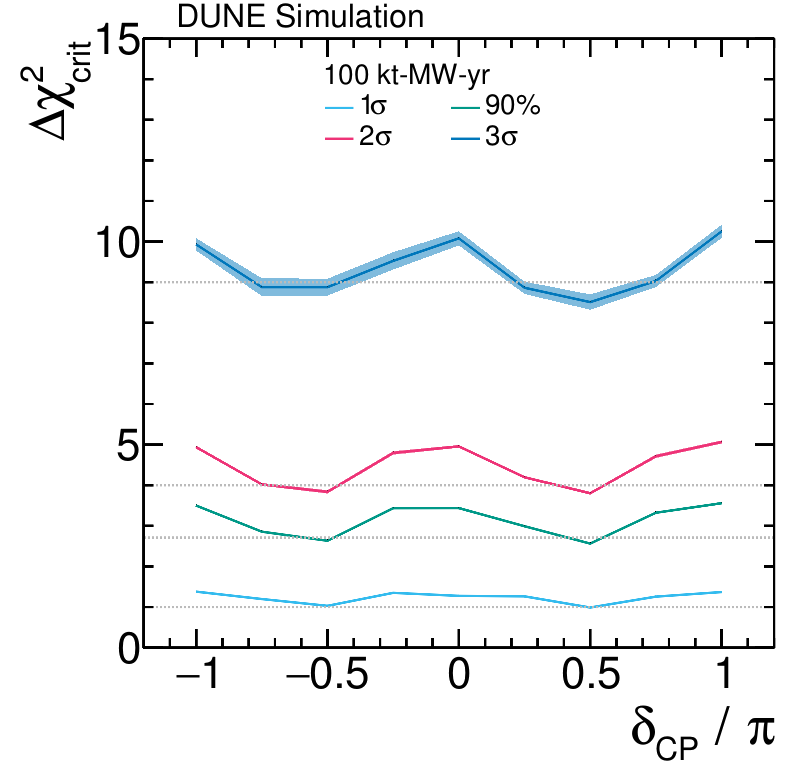
\includegraphics[width=0.8\columnwidth]{dchi2crit_vs_dcp_100ktMWyr.png}}\\
  \subfloat[334 ktMWyr]  {\label{fig:fc_vs_dcp_334}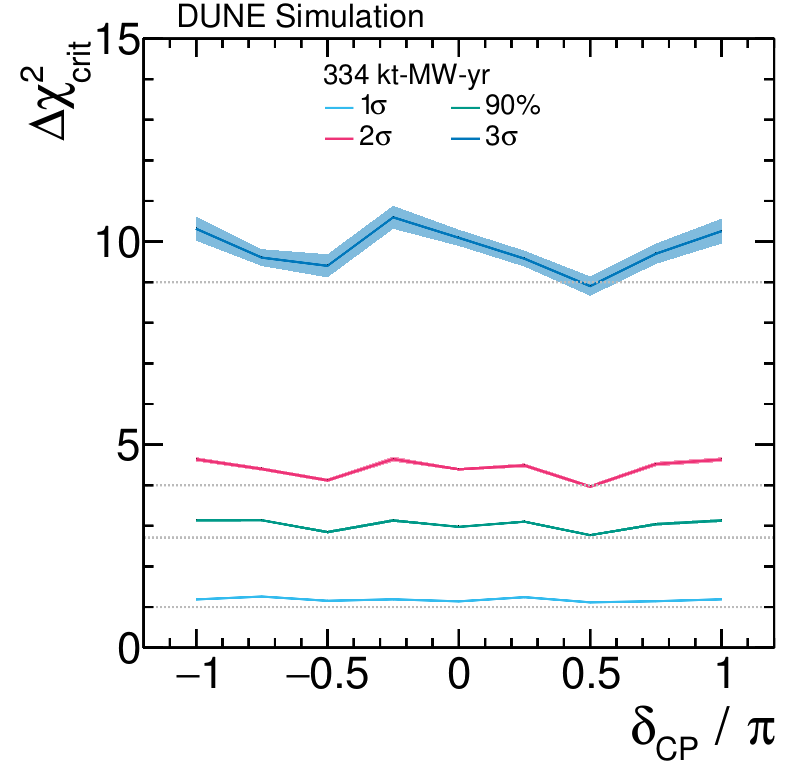
\includegraphics[width=0.8\columnwidth]{dchi2crit_vs_dcp_334ktMWyr.png}}
  \caption{The \dchisqcrit values corresponding to 68.27\% (1$\sigma$), 90\%, 95.45\% (2$\sigma$) and 99.73\% (3$\sigma$) of throws, shown as a function of true \deltacp, for exposures of 100 ktMWyr and 334 ktMWyr. The uncertainty on the \dchisqcrit values is obtained using Equation~\ref{eq:fc_uncertainty}, and is indicated as the shaded line. To guide the eye, horizontal dashed lines are included which indicate the 1$\sigma$, 90\%, 2$\sigma$ and 3$\sigma$ \dchisq values assumed using the constant-\dchisq method, with one degree of freedom. The distribution of throws used produced to calculate the \dchisqcrit values shown are given in Figure~\ref{fig:fc_throws_100ktMWyr} (Figure~\ref{fig:fc_throws_334ktMWyr}) for 100 ktMWyr (334 ktMWyr).}
  \label{fig:fc_vs_dcp}
\end{figure}
As \deltacp is a cyclical parameter, with physical boundaries at $\pm\pi$, it is interesting to see how the \dchisqcrit values evolve as a function of it. Figure~\ref{fig:fc_vs_dcp} shows the \dchisqcrit as a function of true \deltacp, for an ND+FD analysis with an equal FHC:RHC run fraction and a $\theta_{13}$ penalty applied, for 100 ktMWyr and 334 ktMWyr exposures. There is a noticeable, although not large, depression in the \dchisqcrit values at $\deltacp = \pm\pi/2$ for all significance levels considered. This effect is larger at the lower, 100 ktMWyr, exposure, and is larger at higher significance levels. It is also clear from Figure~\ref{fig:fc_vs_dcp} that the \dchisqcrit behaviour is very similar at $\delta = \pm\pi/2$ as at $\deltacp = 0$. Although the \dchisqcrit values are relevant for CPV sensitivity, this evolution of the \dchisqcrit values with \deltacp will be important for estimating DUNE's \deltacp resolution. Details on the number of toy throws used at each point of Figure~\ref{fig:fc_vs_dcp} are given in Appendix~\ref{sec:fc_appendix}, and the toy throw distributions are shown for the 100 ktMWyr (334 ktMWyr) test points in Figure~\ref{fig:fc_throws_100ktMWyr} (Figure~\ref{fig:fc_throws_334ktMWyr}).

\begin{figure*}[htbp]
  \centering
  \subfloat[24 ktMWyr]  {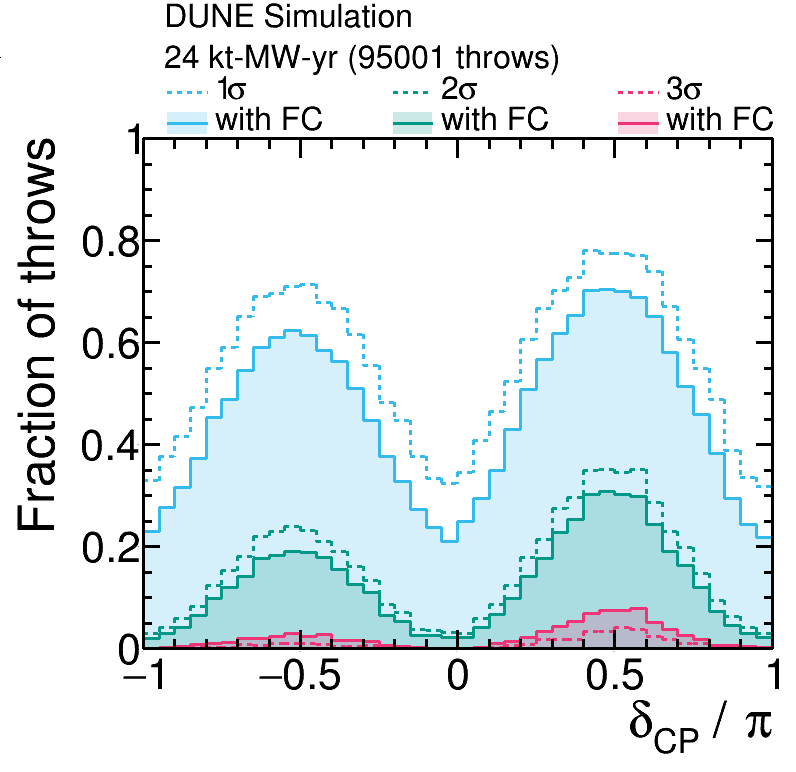
\includegraphics[width=0.33\linewidth]{cpv_throws_withFC_24ktMWyr_NH_th13.png}}
  \subfloat[66 ktMWyr]  {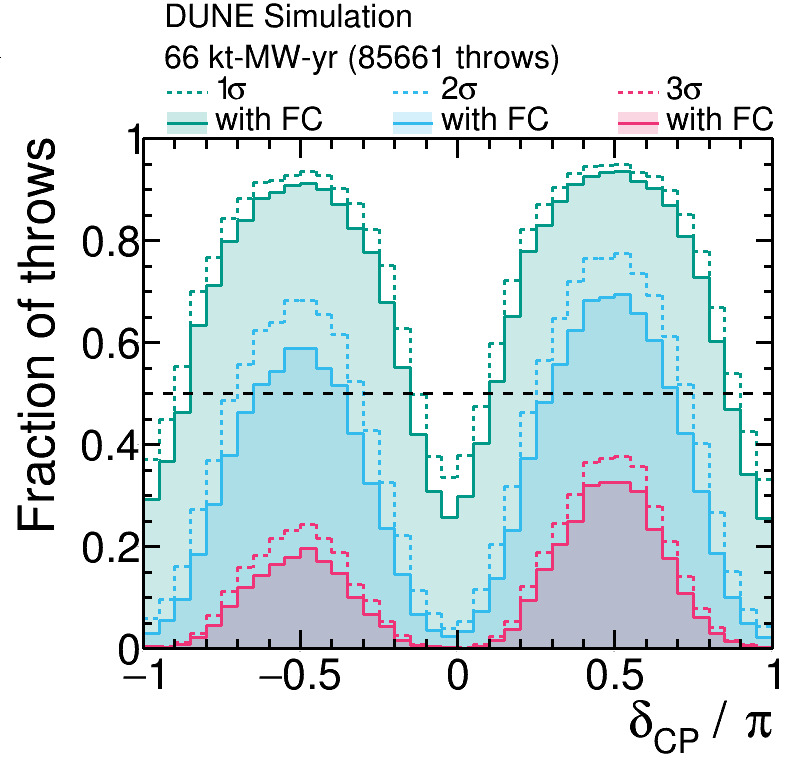
\includegraphics[width=0.33\linewidth]{cpv_throws_withFC_66ktMWyr_NH_th13.png}}
  \subfloat[100 ktMWyr] {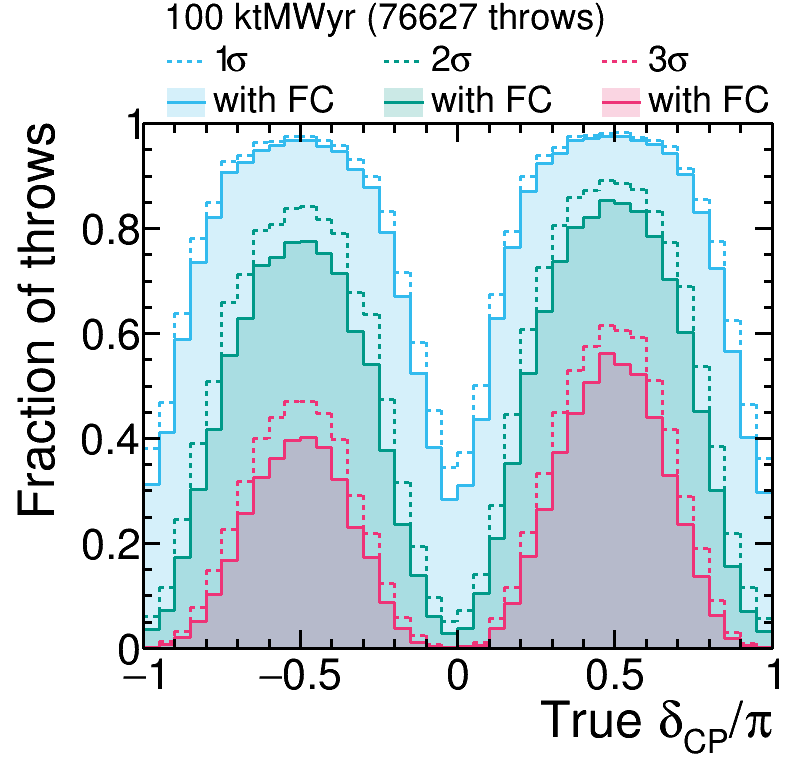
\includegraphics[width=0.33\linewidth]{cpv_throws_withFC_100ktMWyr_NH_th13.png}}\\
  \subfloat[150 ktMWyr] {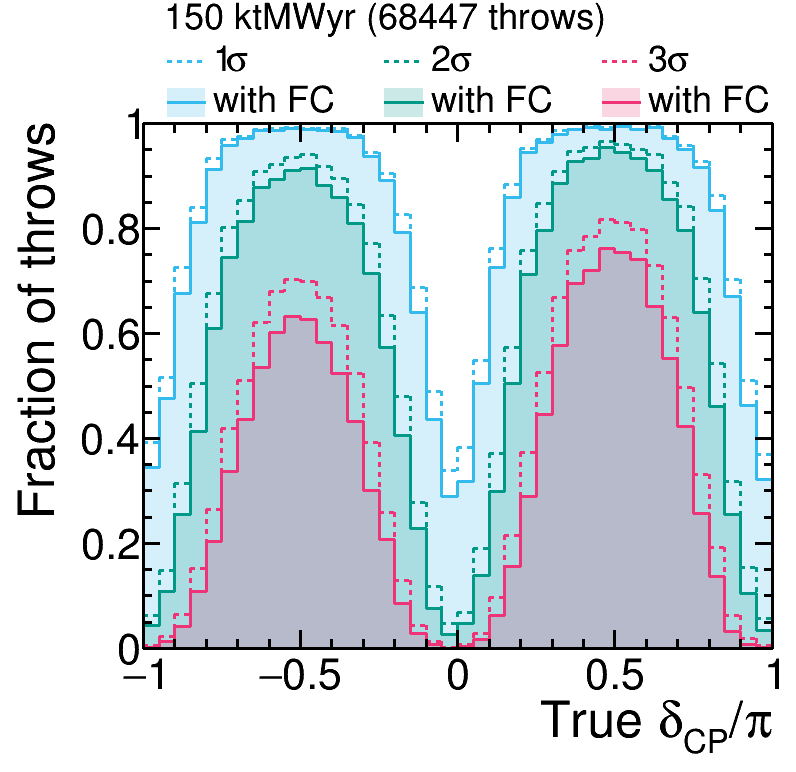
\includegraphics[width=0.33\linewidth]{cpv_throws_withFC_150ktMWyr_NH_th13.png}}
  \subfloat[197 ktMWyr] {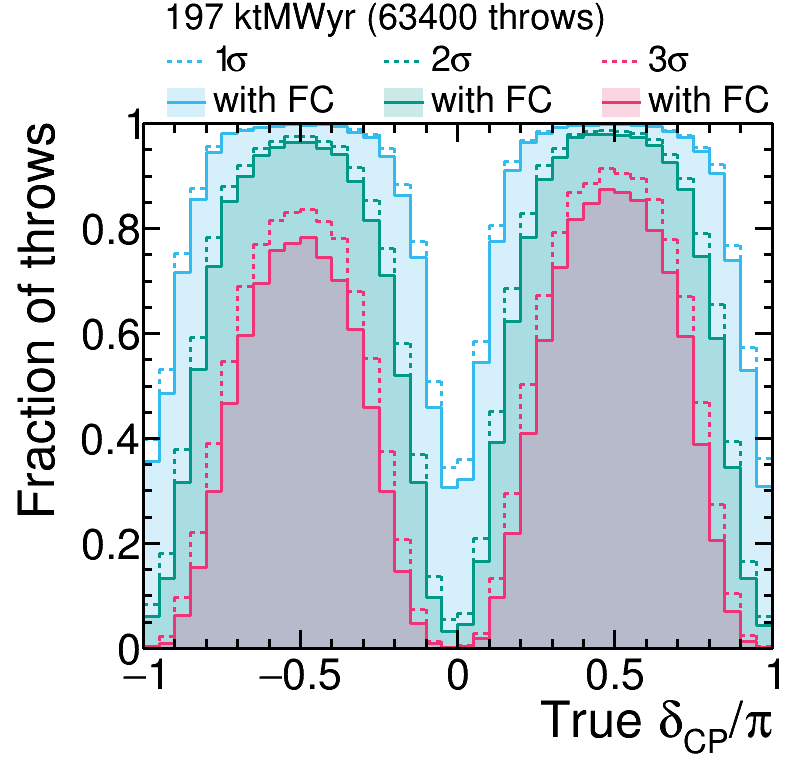
\includegraphics[width=0.33\linewidth]{cpv_throws_withFC_197ktMWyr_NH_th13.png}}
  \subfloat[334 ktMWyr] {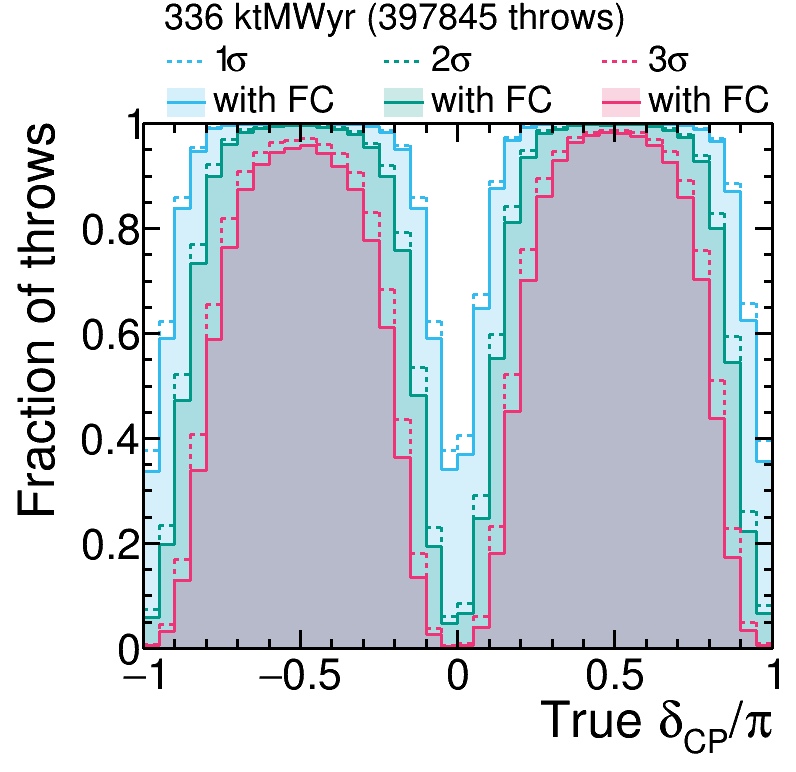
\includegraphics[width=0.33\linewidth]{cpv_throws_withFC_334ktMWyr_NH_th13.png}}
  \caption{Fraction of throws for which the DUNE sensitivity to CP-violation ($\deltacp \neq [0,\pm\pi]$) exceeds 1--3$\sigma$ significance, calculated using constant-\dchisq (dashed lines) and \dchisqcrit values calculated using the Feldman-Cousins method (shaded histograms), as a function of the true value of \deltacp. Shown for NO, for a number of different exposures. The number of throws used to make each figure is also shown.}
  \label{fig:cpv_over_time_fc}
\end{figure*}
Having calculated the \dchisqcrit values necessary to achieve correct coverage, it is possible to re-evaluate the CPV sensitivity previously shown assuming a constant \dchisq method in Figure~\ref{fig:cpv_over_time}. Figure~\ref{fig:cpv_over_time_fc} shows the 1, 2 and 3$\sigma$ CPV sensitivities as a function of true \deltacp, with and without the Feldman-Cousins correction (e.g., the \dchisqcrit values given in Figure~\ref{fig:fc_vs_exp} applied). The uncorrected values are the same as in Figure~\ref{fig:cpv_over_time}. In general, the effect of the Feldman-Cousins correction is to reduce the fraction of toy throws that cross each significance threshold, by a maximum of $\sim$10\%, but the eact fraction changes as a function of true \deltacp value and exposure. An exception to this general trend is the 3$\sigma$ behaviour at 24 ktMWyr, the lowest exposure shown, where the significance increases. This can be understood because of the rise in the 3$\sigma$ \dchisqcrit value at low exposures observed in Figure~\ref{fig:fc_vs_exp}.

\begin{figure*}[htbp]
  \centering
  \subfloat[$\deltacp = -\pi/2$] {\includegraphics[width=0.8\columnwidth]{{fraction_throws_vs_exp_dcp-0.5_FC}.pdf}}
  \subfloat[$\deltacp = +\pi/2$] {\includegraphics[width=0.8\columnwidth]{{fraction_throws_vs_exp_dcp0.5_FC}.pdf}}
  \caption{Fraction of throws for which the DUNE sensitivity to CP-violation ($\deltacp \neq [0,\pm\pi]$) exceeds 1--3$\sigma$ significance, at $\deltacp = \pm\pi/2$, calculated using constant-\dchisq (dashed lines) and \dchisqcrit values calculated using the Feldman-Cousins methed (shaded histograms), as a function of exposure.}
  \label{fig:cpv_vs_exp_fc}
\end{figure*}
Figure~\ref{fig:cpv_vs_exp_fc} shows the fraction of throws which exceed different significance thresholds at the maximal \deltacp violation values of $\pm\pi/2$, as a function of exposure, with and without Feldman-Cousins corrections, for 1--3$\sigma$ significance values. It is clear from Figure~\ref{fig:cpv_vs_exp_fc} that the effect of the correction is not large, and $\sim$10\% longer exposures are required for the median sensitivity to cross each significance threshold than without correction, at both points shown.

\FloatBarrier

\section{Neutrino mass ordering sensitivity}
\label{sec:mh_sens}

In this section, the toy-throwing approach described in Section~\ref{sec:analysis_framework} is used to explore the neutrino mass ordering sensitivity as a function of exposure in detail. In all cases, a joint ND+FD fit is performed, and the reactor $\theta_{13}$ constraint is always applied, as described in Section~\ref{sec:analysis_framework}. An equal split between FHC and RHC running is assumed based on the results obtained in Section~\ref{sec:run_plan_opt}.

\begin{figure}[htbp]
  \centering
  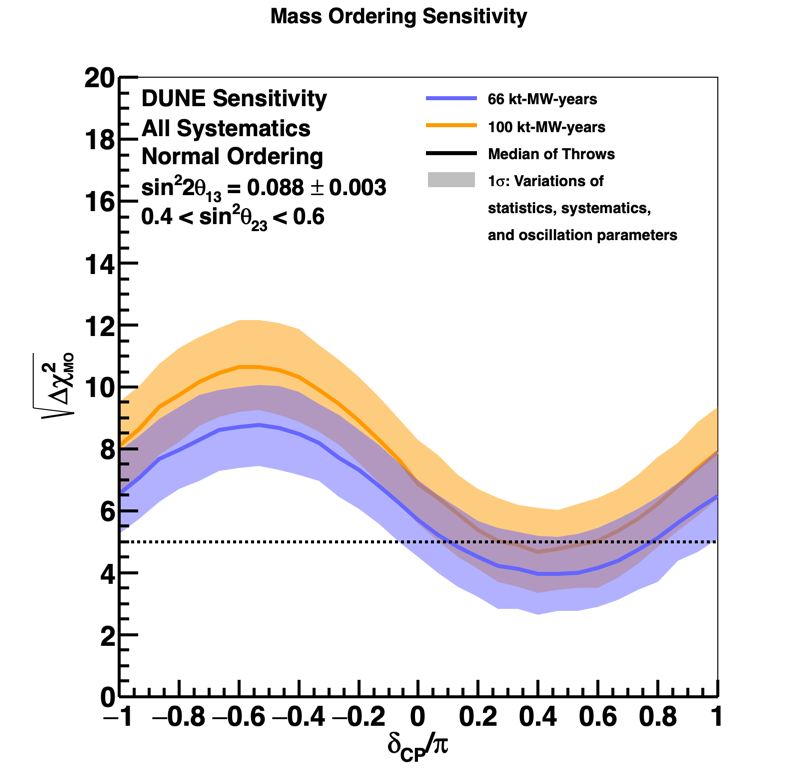
\includegraphics[width=0.8\linewidth, trim={0cm 0cm 0cm 2.3cm}, clip]{mh_two_exps_throws_nh_2019_v4_lowexp.png}
  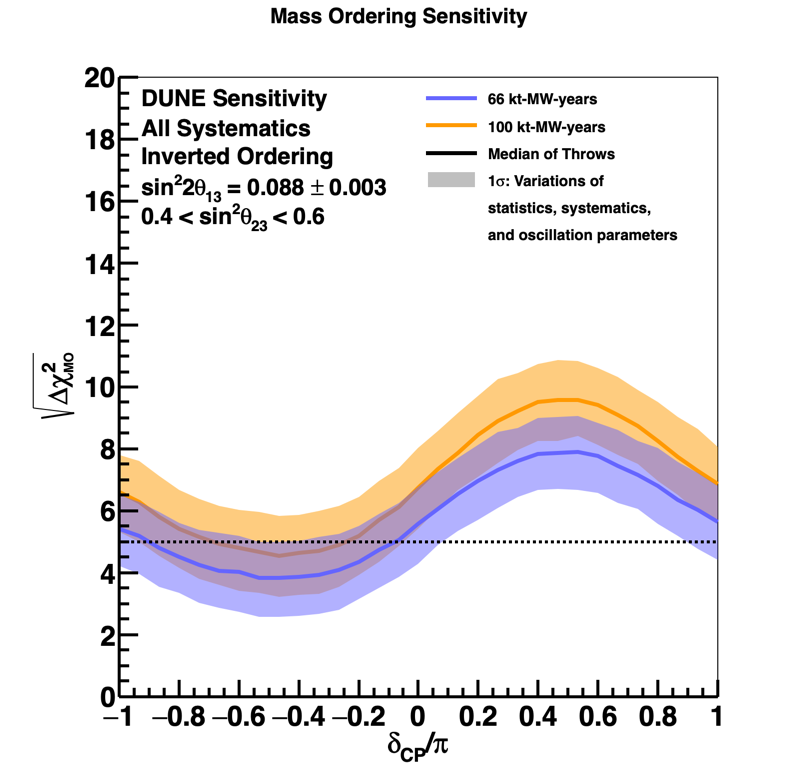
\includegraphics[width=0.8\linewidth, trim={0cm 0cm 0cm 2.3cm}, clip]{mh_two_exps_throws_ih_2019_v4_lowexp.png}
  \caption{Significance of the DUNE determination of the neutrino mass ordering, as a function of the true value of \deltacp, for 66 kt-MW-yrs (blue) and 100 kt-MW-yrs (orange) exposures. The width of the transparent bands cover 68\% of fits in which random throws are used to simulate systematic, oscillation parameter and statistical variations, with independent fits performed for each throw constrained by pre-fit uncertainties. The solid lines show the median significance.}
  \label{fig:mh_bands}
\end{figure}
Figure~\ref{fig:mh_bands} shows the significance with which the neutrino mass ordering can be determined for both true NO and IO, for exposures of 66 and 100 kt-MW-yrs. The sensitivity metric used is the square root of the difference between the best fit $\chi^{2}$ value obtained using each ordering, as shown in Equation~\ref{eq:mh_chi2}, which is calculated for each throw of the systematic, other oscillation parameters and statistics. The characteristic shape of the MH sensitivity in Figure~\ref{fig:mh_bands} results from near degeneracy between matter and CPV effects that occurs near $\deltacp=\pi/2$ ($-\deltacp=\pi/2$) for true normal (inverted) ordering. We note that dedicated studies have shown that special attention must be paid to the statistical interpretation of neutrino mass ordering sensitivities~\cite{Ciuffoli:2013rza,Qian:2012zn,Blennow:2013oma} because the \dchisq metric does not follow the expected chi-square distribution for one degree of freedom, so the interpretation of the $\sqrt{\dchisq}$ as the sensitivity is complicated.

\begin{figure*}[htbp]
  \centering
  \subfloat[6 kt-MW-yrs]   {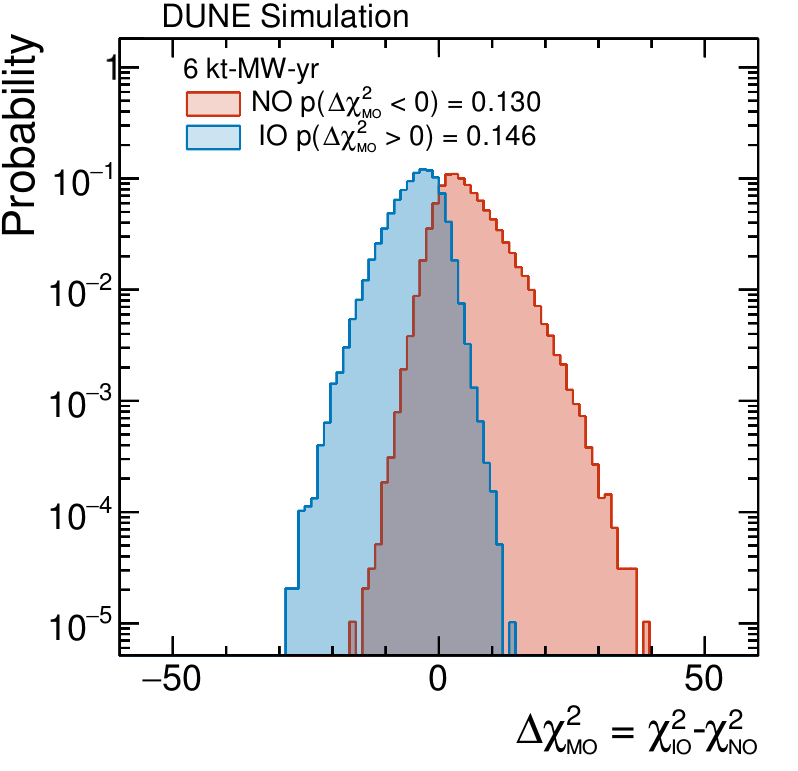
\includegraphics[width=0.33\linewidth]{MH_comp_ndfd_6ktMWyr_th13.png}}
  \subfloat[12 kt-MW-yrs]  {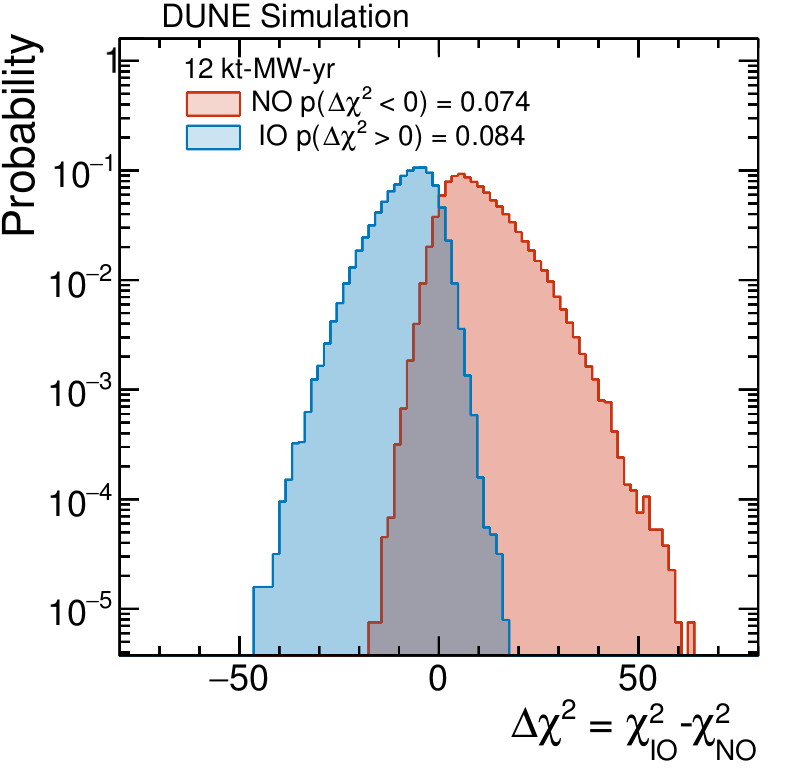
\includegraphics[width=0.33\linewidth]{MH_comp_ndfd_12ktMWyr_th13.png}}
  \subfloat[24 kt-MW-yrs]  {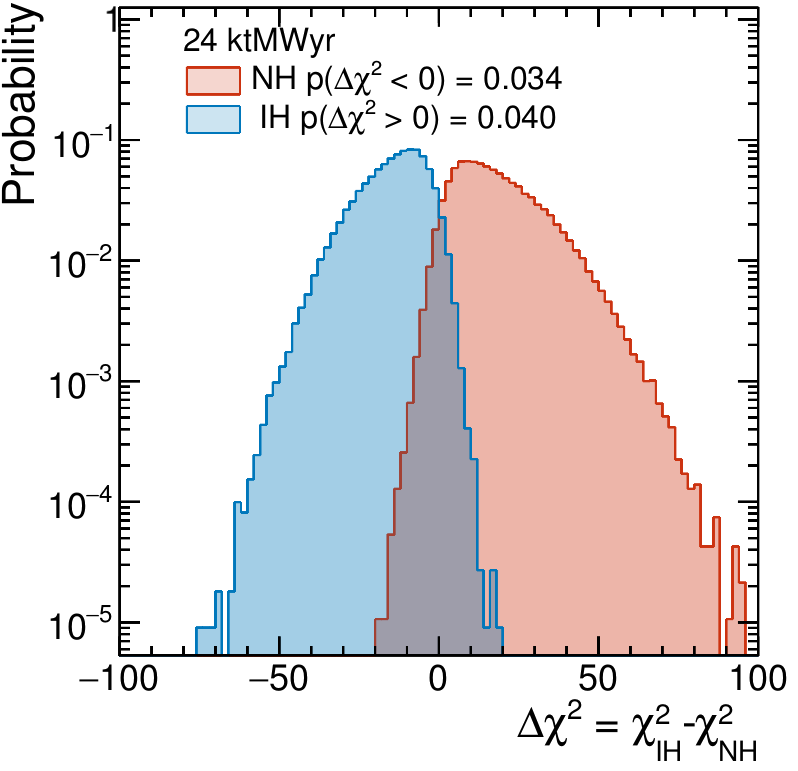
\includegraphics[width=0.33\linewidth]{MH_comp_ndfd_24ktMWyr_th13.png}}\\
  \subfloat[66 kt-MW-yrs]  {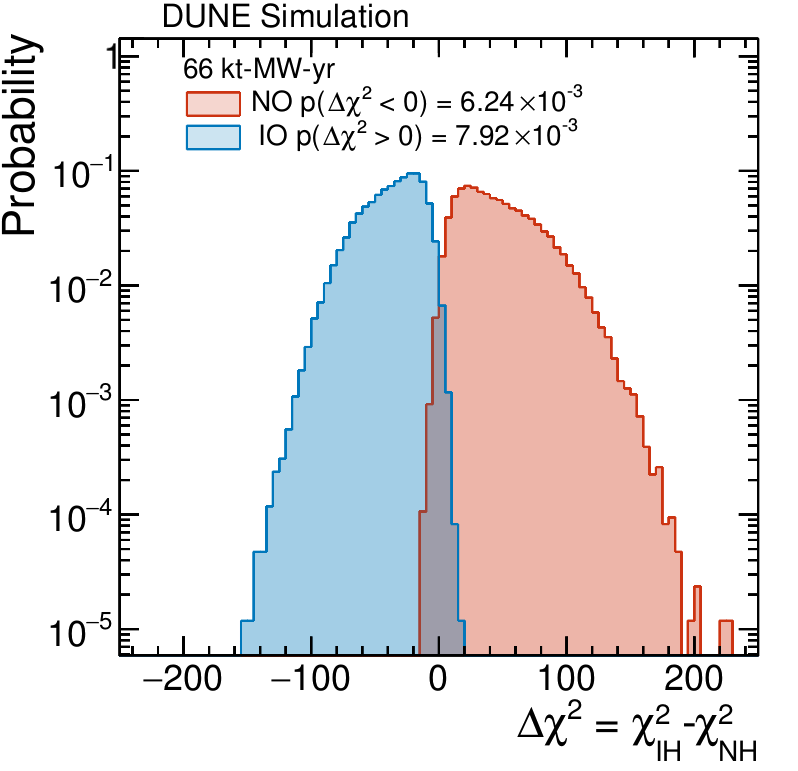
\includegraphics[width=0.33\linewidth]{MH_comp_ndfd_66ktMWyr_th13.png}}
  \subfloat[100 kt-MW-yrs] {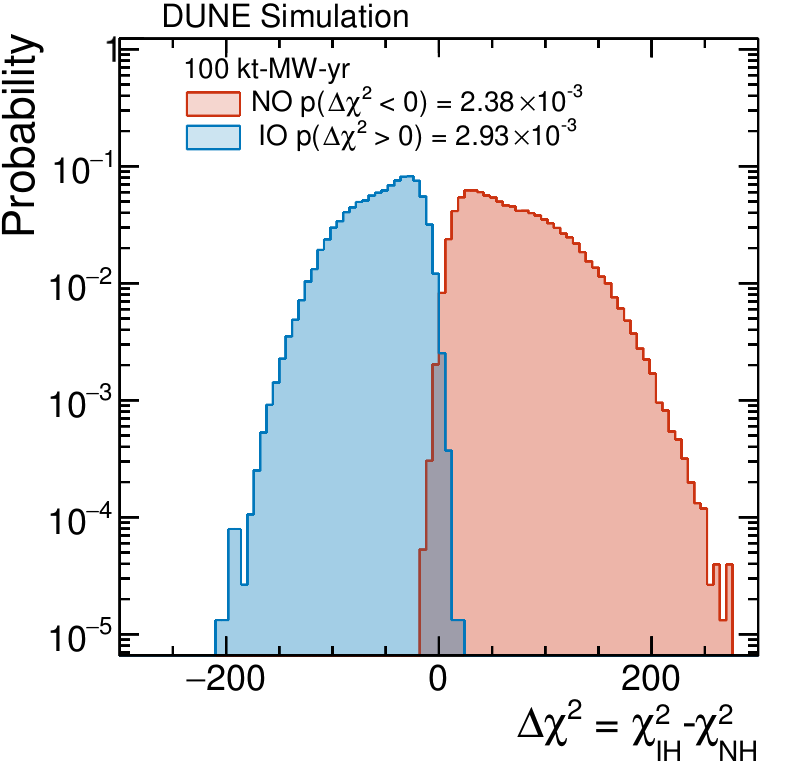
\includegraphics[width=0.33\linewidth]{MH_comp_ndfd_100ktMWyr_th13.png}}
  \subfloat[334 kt-MW-yrs] {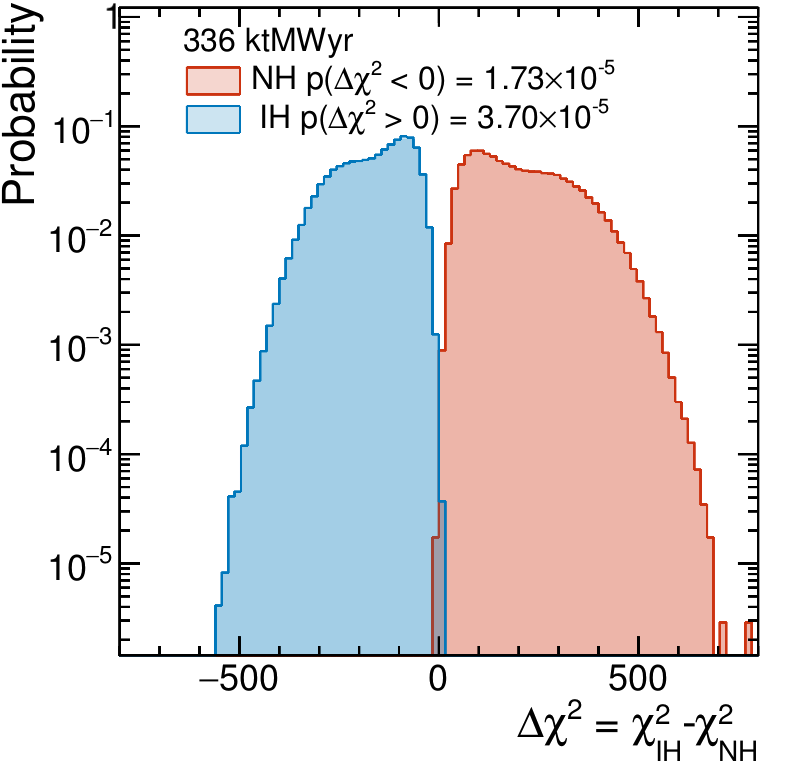
\includegraphics[width=0.33\linewidth]{MH_comp_ndfd_334ktMWyr_th13.png}}
  \caption{The distribution of $\dchisq = \chi^{2}_{\mathrm{IO}} - \chi^{2}_{\mathrm{NO}}$ values shown for both true normal (red) and true inverted (blue) hierarchies built using random throws of the systematic parameters, the oscillation parameters and with statistical variations. In each case, the $\chi^{2}$ values are separately minimized with respect to all variable parameters before calculating the test statistic. The fraction of throws for which the value of \dchisq is greater than (less than) 0 is also given for inverted (normal) hierarchies. For each ordering and exposure, approximately 100,000 throws were used.}
  \label{fig:mh_comp_over_time}
\end{figure*}
Given the complications with the interpretation of significance for mass ordering determination, it is instructive to look at the distribution of the test-statistic (Equation~\ref{eq:mh_chi2}), which gives more information than the 68\% central band and median throw shown in Figure~\ref{fig:mh_bands}. Figure~\ref{fig:mh_comp_over_time} shows the distribution of \dchisq obtained for a large ensemble of throws, for both true and inverted orderings, for a number of different exposures. Note that there is a uniform distribution of true \deltacp used in the throws at each exposure. The change in shape at higher exposures in Figure~\ref{fig:mh_comp_over_time} is due to the relationship with \deltacp, and as might be expected from Figure~\ref{fig:mh_bands}, the separation between hierarchies is greater for some true values of \deltacp than others. Note that this additional structure starts to become obvious from a $\sim$66 kt-MW-yrs exposure, at which point the CPV sensitivity is not very strong (see Section~\ref{sec:cp_sens}). For all exposures, the shape of the throw distribution is highly non-Gaussian, which makes it difficult to apply simple corrections to the sensitivity of the sort described in Ref.~\cite{Blennow:2013oma}. As a result we do not explore alternatives to $\sqrt{\dchisq}$ as a sensitivity metric, but note that the full information is given in Figure~\ref{fig:mh_comp_over_time}.

Figure~\ref{fig:mh_comp_over_time} also indicates the probability for the test statistic \dchisq to be less (more) than zero from the toy throws for true normal (inverted) hierarchies at each exposure. This marks the proportion of toys which appear more like the incorrect ordering than the true ordering for the toy. However, it is not easily converted to a single number sensitivity, although it does indicate the risk of a type I/type II error if the \dchisq value obtained by an experiment is exactly zero. It is clear from Figure~\ref{fig:mh_comp_over_time} that DUNE is sensitive to the mass ordering even from very low ($\sim$10 kt-MW-yrs) exposures, and by exposures of 66 kt-MW-yrs, the overlap between the orderings is very small.

\begin{figure*}[htbp]
  \centering
  \subfloat[6 kt-MW-yrs]   {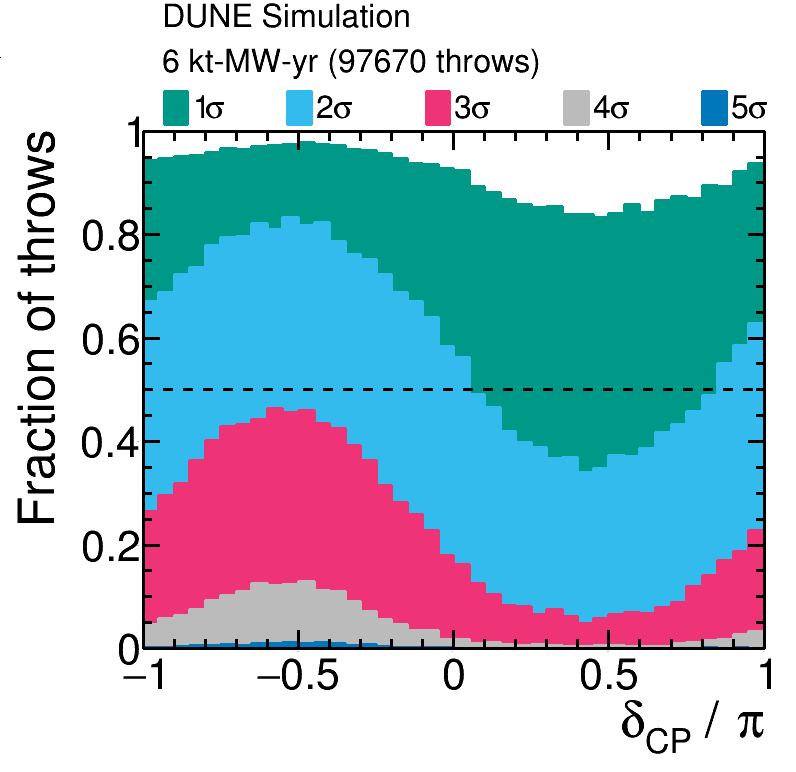
\includegraphics[width=0.33\linewidth]{mh_throws_6ktMWyr_NH_th13.png}}
  \subfloat[12 kt-MW-yrs]  {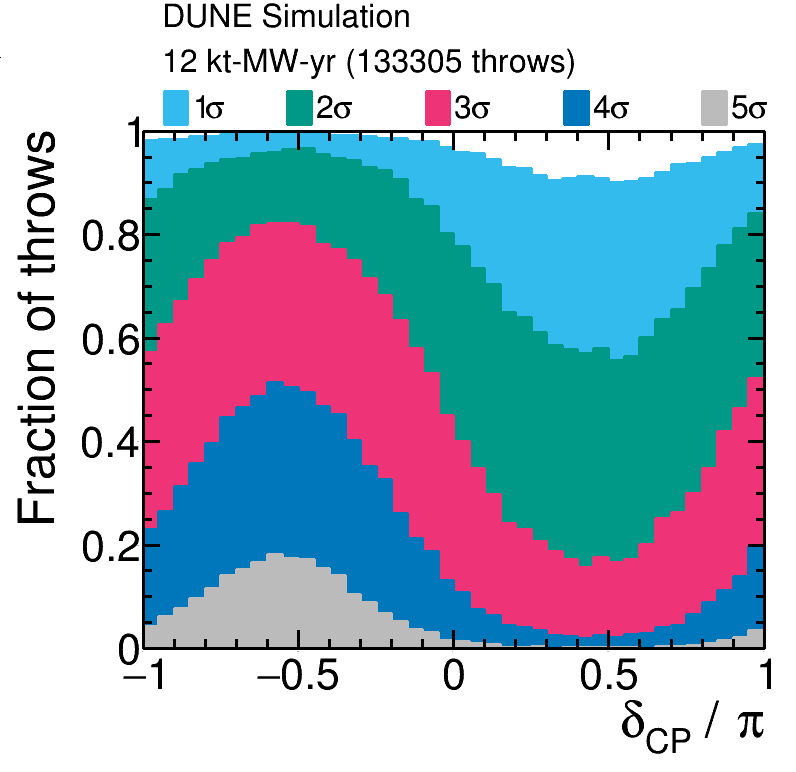
\includegraphics[width=0.33\linewidth]{mh_throws_12ktMWyr_NH_th13.png}}
  \subfloat[24 kt-MW-yrs]  {\includegraphics[width=0.33\linewidth]{mh_throws_24ktMWyr_NH_th13.png}}\\
  \subfloat[66 kt-MW-yrs]  {\includegraphics[width=0.33\linewidth]{mh_throws_66ktMWyr_NH_th13.png}}
  \subfloat[100 kt-MW-yrs] {\includegraphics[width=0.33\linewidth]{mh_throws_100ktMWyr_NH_th13.png}}
  \subfloat[334 kt-MW-yrs] {\includegraphics[width=0.33\linewidth]{mh_throws_334ktMWyr_NH_th13.png}}
  \caption{Fraction of throws for which the DUNE sensitivity to the mass ordering exceeds 1--5$\sigma$ significance, as a function of the true value of \deltacp. Shown for NO, for a number of different exposures. The number of throws used to make each figure is also shown.}
  \label{fig:mh_nh_over_time}
\end{figure*}

Figure~\ref{fig:mh_nh_over_time} shows an alternative way to present the result of the throws as a function of \deltacp, which is complementary to Figure~\ref{fig:mh_bands}. The fraction of throws for which the simple figure of merit (the square-root of Equation~\ref{eq:mh_chi2}) exceeds different confidence levels are shown, for 1--5$\sigma$ significances, and a variety of exposures, all for true NO. The same throws are used as in Figures~\ref{fig:mh_comp_over_time}. The highest exposure shown, 334 kt-MW-yrs, corresponds to the seven-year exposure using the nominal staging scenario in Ref.~\cite{Abi:2020qib}. Despite the caveats regarding the intepretation of $\sqrt{\dchisq}$ as units of $\sigma$, the general trend is clear, and provides more information about the expected DUNE sensitivity at low exposures. As with Figure~\ref{fig:cpv_over_time}, the point at which the median significance (50\% of throws) passes different significance thresholds can be easily read from the figures, and can be compared with those shown in Figure~\ref{fig:mh_bands}. The same general shape as a function of \deltacp as was observed in Figure~\ref{fig:mh_bands} can be seen. The general trend would be very similar in IO, reflected in the line $\deltacp = 0$. The median significance for $\deltacp = -\pi/2$ exceeds 5$\sigma$ for 24 kt-MW-yrs, at which point the fraction of throws for which the significance is 3$\sigma$ or greater is small, $\sim$2\%. By 66 kt-MW-yrs, 100\% of the throws exceed 5$\sigma$ at $\deltacp = -\pi/2$. By 100 kt-MW-yrs exposures, the median significance for all true values of \deltacp exceeds 5$\sigma$. At long exposures of 334 kt-MW-yrs, almost 100\% of the throws exceed 5$\sigma$ for all values of \deltacp.

\section{Conclusion}
\label{sec:conclude}

In this work we have presented a detailed exploration of DUNE's sensitivity to CPV and the mass ordering at low exposures. The analysis uses the same framework, flux, cross section and detector models and selections as were used in Ref.~\cite{Abi:2020qib}, which showed the ultimate DUNE sensitivity to CPV, MO and other oscillation parameters, with large statistics samples after long exposures.

\todo{Add comment about run plan optimization...}

The studies presented here demonstrate that a full treatment of DUNE's sensitivity at low exposures supports the conclusions made in Refs.~\cite{Abi:2020qib} and~\cite{Abi:2020evt} using simple Asimov studies. In particular, the median CPV sensitivity is $\sim$3$\sigma$ for $\deltacp = \pm\pi/2$ after approximately a 100 ktMWyr FD exposure. We also explore the variations in the expected sensitivity around the median value. Additionally, we show that the CPV sensitivity is not significantly degraded when Feldman-Cousins corrections are included, leading to $\sim$10\% longer exposures to reach a given significance level. Crucially, we find that after an initial low-exposure rise, the Feldman-Cousins \dchisqcrit do not change as a function of exposure, as has been observed by the T2K experiment~\cite{Abe:2021gky}.

We have also shown that strong statements on the mass ordering can be expected with very short exposures of $\sim$12 ktMWyr, which supports the results shown in Refs.~\cite{Abi:2020qib} and~\cite{Abi:2020evt} with a more complete treatment of the systematic uncertainty.

We note that although the analysis used here makes no assumptions about the FD staging scenario, and results are given as a function of exposure only, the results are dependent on having a performant ND complex from the start of the experiment. In particular, the low-exposures necessary to make world-leading statements about the mass hierarchy can only be given with confidence with ND samples included in the fit. We note also that additional samples of events from other detectors in the DUNE ND complex are not explicitly included in this analysis, but there is an assumption that we will be able to control the uncertainties to the level used in the analysis, and it should be understood that that implicitly relies on having a highly capable ND.

\begin{acknowledgements}
This document was prepared by the DUNE collaboration using the
resources of the Fermi National Accelerator Laboratory 
(Fermilab), a U.S. Department of Energy, Office of Science, 
HEP User Facility. Fermilab is managed by Fermi Research Alliance, 
LLC (FRA), acting under Contract No. DE-AC02-07CH11359.
%
% Funding agencies, alphabetical by country, then alphabetical by agency name
%
This work was supported by
CNPq,
FAPERJ,
FAPEG and 
FAPESP,                         Brazil;
CFI, 
IPP and 
NSERC,                          Canada;
CERN;
M\v{S}MT,                       Czech Republic;
ERDF, 
H2020-EU and 
MSCA,                           European Union;
CNRS/IN2P3 and
CEA,                            France;
INFN,                           Italy;
FCT,                            Portugal;
NRF,                            South Korea;
CAM, 
Fundaci\'{o}n ``La Caixa'',
Junta de Andaluc\'ia-FEDER, and 
MICINN,                         Spain;
SERI and 
SNSF,                           Switzerland;
T\"UB\.ITAK,                    Turkey;
The Royal Society and 
UKRI/STFC,                      United Kingdom;
DOE and 
NSF,                            United States of America.
This research used resources of the 
National Energy Research Scientific Computing Center (NERSC), 
a U.S. Department of Energy Office of Science User Facility 
operated under Contract No. DE-AC02-05CH11231.
\end{acknowledgements}

\bibliographystyle{utphys}
\bibliography{common/tdr-citedb}

\end{document}
